% !TeX program = xelatex
\documentclass[9pt]{beamer}

\mode<presentation>
{
 \usetheme{JuanLesPins}
 \usefonttheme{serif}
 \usecolortheme{beaver}
 \setbeamercovered{invisible} \setbeamertemplate{blocks}[rounded][shadow=true] 
 \setbeamertemplate{navigation symbols}{} 
 \setbeamertemplate{footline}[frame number]
 \usecolortheme[RGB={122,4,24}]{structure}
}

\setcounter{tocdepth}{1}


%\usepackage{fancybox}
%\usepackage{graphicx}
%\usepackage{colortbl}
%\usepackage{textcomp}
%\usepackage{multirow}
%\usepackage{calligra}
%\usepackage{srcltx}
%\usepackage{enumerate}
%\newcommand{\degree}{\ensuremath{^\circ}}
%\newcommand{\xmark}{\ding{55}}
%\usepackage{multimedia}
%\usepackage{esvect}

%%%%%%%%%%%%%%%%%%%%%%%%%%%%%%%%%%%%%%%%%%%
%%%%%%%%%%%%%%%%%%%%%%%%%%%%%%%%%%%%%%%%%%%
%%%%%%%%%%%%%%%%% PACKAGES %%%%%%%%%%%%%%%%%

% BASICAO

\usepackage{lmodern}
\usepackage[T1]{fontenc}
\usepackage[useregional]{datetime2}

% Para usar com PDFTEX
%\usepackage[brazilian]{babel}
%\usepackage[utf8]{inputenc}

% Para usar com XELATEX
\usepackage{polyglossia}
\setdefaultlanguage{brazil}


% FIGURAS
\usepackage{graphicx,float}
\usepackage{booktabs, longtable}


% TABELAS E DIAGRAMAÇÃO
\usepackage{enumerate}
\usepackage{multirow,multicol}
\usepackage{makecell}
\usepackage{array}
%\usepackage{fancybox}
%\usepackage{colortbl}

\renewcommand{\arraystretch}{1.2}

% ?????????????

% Fonte Courier?
%\usepackage{courier}

% Simbolos
%\usepackage{textcomp}

% Texto caligrafico
%\usepackage{calligra}

% Conexão entre pdfs e dvis
%\usepackage{srcltx}

% Para delimitar environments de tipo float
%\usepackage{cprotect}

% Para texto literal (programação)
%\usepackage{verbatim}

% Pegar números relacionados a referências para uso
%\usepackage{refcount}

% Para colocar relógios de ponteiro
%\usepackage{tdclock}

%%%%%%%%%%%%%%%%%%%%%%%%%%%%%%%%%%%%%%%%%%%
%%%%%%%%%%%%%%%%%%%%%%%%%%%%%%%%%%%%%%%%%%%
%%%%%%%%%%%%%%%%% COISAS MATEMATICAS %%%%%%%%%%%%%%%%%

\usepackage{amsmath,amssymb,amsfonts,xfrac,cancel,bm,mathtools}

% Notação de ângulos para complexos
%\usepackage{steinmetz}

% Notação de derivadas
%\usepackage[thinc]{esdiff}
%\usepackage{commath}

% Setinhas para notação de vetor
%\usepackage{esvect}

% Negrito para notação de vetor
\renewcommand{\vec}[1]{\mathbf{#1}}

% Fonte para notação em rsfs
%\usepackage{mathrsfs}

% Para mapas de karnaugh
%\usepackage{karnaugh-map}


% setup do (circui)tikz
\usepackage[american, nooldvoltagedirection, siunitx,
cuteinductors]{circuitikz}

% Comando para mudar escala das tikzpictures \setmyunit{length}
\newcommand{\setmyunit}[1]{\tikzset{every picture/.style={x=#1, y=#1}}}

\setmyunit{2cm}

% Unidades (inclusa no circuitikz)
%\usepackage{siunitx}

\usepackage{tikz}
\usetikzlibrary{positioning, calc,
patterns, arrows.meta, decorations.pathmorphing,decorations.pathreplacing,angles,quotes,intersections}


\tikzset{ang/.style={draw, angle radius=15pt,angle eccentricity=1.3}}

%\newlength{\ladderskip}
%\setlength{\ladderskip}{5\tikzcircuitssizeunit} % 5\tikzcircuitssizeunit = 35pt
%\newlength{\ladderrungsep}
%\setlength{\ladderrungsep}{.2\ladderskip}
%\def\ladderrungend#1{\pgftransformyshift{-#1\ladderskip-\ladderrungsep}}
%\newcommand{\powerrails}[1][0.7]{\draw let \p1=(laddertopright) in
%	(0,\y1+#1\ladderskip) -- (0,\ladderskip)
%	(\x1,\y1+#1\ladderskip) -- (\x1,\ladderskip);}

% Cores (inclusa no tikz)
%\usepackage{xcolor}


%%%%%%%%%%%%%%%%%%%%%%%%%%%%%%%%%%%%%%%%%%%
%%%%%%%%%%%%%%%%%%%%%%%%%%%%%%%%%%%%%%%%%%%
%%%%%%%%%%%%%%%%% COISAS DOIDAS %%%%%%%%%%%%%%%%%

% setup do siunitx
\sisetup{per-mode=symbol,output-decimal-marker={,},math-micro=\text{µ},text-micro=µ,exponent-product = \cdot,math-ohm=\Omega,
	text-ohm=\ensuremath{\Omega}}

% MATLAB
%\usepackage{xspace}
%\newcommand{\MATLAB}{\textsc{Matlab}\xspace}

% Notação de negação lógica
\newcommand{\notted}[1]{%
	\overline{#1}%
}

% Padrões de linhas que não funcionam no overleaf

%\pgfdeclarepatternformonly{south east lines}{\pgfqpoint{-0pt}{-0pt}}{\pgfqpoint{3pt}{3pt}}{\pgfqpoint{3pt}{3pt}}{
%	\pgfsetlinewidth{0.4pt}
%	\pgfpathmoveto{\pgfqpoint{0pt}{3pt}}
%	\pgfpathlineto{\pgfqpoint{3pt}{0pt}}
%	\pgfpathmoveto{\pgfqpoint{.2pt}{-.2pt}}
%	\pgfpathlineto{\pgfqpoint{-.2pt}{.2pt}}
%	\pgfpathmoveto{\pgfqpoint{3.2pt}{2.8pt}}
%	\pgfpathlineto{\pgfqpoint{2.8pt}{3.2pt}}
%	\pgfusepath{stroke}}
%
%\pgfdeclarepatternformonly{south west lines}{\pgfqpoint{-0pt}{-0pt}}{\pgfqpoint{3pt}{3pt}}{\pgfqpoint{3pt}{3pt}}{
%	\pgfsetlinewidth{0.4pt}
%	\pgfpathmoveto{\pgfqpoint{0pt}{0pt}}
%	\pgfpathlineto{\pgfqpoint{3pt}{3pt}}
%	\pgfpathmoveto{\pgfqpoint{2.8pt}{-.2pt}}
%	\pgfpathlineto{\pgfqpoint{3.2pt}{.2pt}}
%	\pgfpathmoveto{\pgfqpoint{-.2pt}{2.8pt}}
%	\pgfpathlineto{\pgfqpoint{.2pt}{3.2pt}}
%	\pgfusepath{stroke}}


% cor do fundo do block
%\definecolor{mWhite}{RGB}{239, 230, 231}

% Definições de funções trinométricas em pt-br
\DeclareMathOperator{\sen}{sen}
\DeclareMathOperator{\tg}{tg}
\DeclareMathOperator{\cotg}{cotg}
\DeclareMathOperator{\cossec}{cossec}

% QED branco
%\newcommand*{\QEDB}{\hfill\ensuremath{\square}}

% estilos para diagrama de blocos
%\newcommand{\deftkzbds}{
%	\tikzstyle{block} = [draw, fill=blue!20, rectangle, minimum height=3em, minimum width=6em]
%	\tikzstyle{sum} = [draw, fill=blue!20, circle, node distance=1cm]
%	\tikzstyle{input} = [coordinate]
%	\tikzstyle{output} = [coordinate]
%	\tikzstyle{pinstyle} = [pin edge={to-,thin,black}]
%}

% tipo de coluna matemática centralizada
%\newcolumntype{C}{>{$}c<{$}}

% para marcar ponto na tela e desenhar sobre
\newcommand{\tikzmark}[1]{\tikz[baseline,remember picture] \coordinate (#1) {};}

% unidades uteis para siuntix

\DeclareSIUnit{\voltef}{V_{ef}}
\DeclareSIUnit{\cons}{\newton\meter\squared\per\coulomb\squared}
%\DeclareSIUnit{\lbf}{lbf}
%\DeclareSIUnit{\kgf}{kgf}
%\DeclareSIUnit{\kgfp}{\kgf \per \centi\meter\squared}
%\DeclareSIUnit{\mca}{mca}
%\DeclareSIUnit{\barp}{bar}
%\DeclareSIUnit{\pol}{pol}
%\DeclareSIUnit{\psip}{psi}
%\DeclareSIUnit{\atm}{atm}
%\DeclareSIUnit{\HP}{HP}
%\DeclareSIUnit{\psid}{\lbf\per\pol\squared}
%\DeclareSIUnit{}{}

% Usar para diminuir espaçamento antes/depois da equação (\useshortskip)
%\usepackage{nccmath}
%\usepackage{xpatch}
%\xpatchcmd{\NCC@ignorepar}{%
%	\abovedisplayskip\abovedisplayshortskip}
%{%
%	\abovedisplayskip\abovedisplayshortskip%
%	\belowdisplayskip\belowdisplayshortskip}
%{}{}
%
%\usepackage{chngcntr}
%\counterwithin*{equation}{section}
%\newcounter{saveenumi}
%\newcommand{\saveenumerate}{%
%	\stepcounter{saveenumi}%
%	\label{saveenumi-\thesaveenumi}}
%\newcommand{\restoreenumerate}{%
%	\setcounterref{enumi}{saveenumi-\thesaveenumi}}

% Símbolo para graus (usar \ang{degrees} do package siunitx)
%\newcommand{\degree}{\ensuremath{^\circ}}

% X de errado e certinho correspondente
\usepackage{pifont}
\newcommand{\cmark}{\ding{51}}%
\newcommand{\xmark}{\ding{55}}%

% \itemequation[label]{text before}{equation}

%\makeatletter
%\newcommand*{\itemequation}[3][]{%
%  \item
%  \begingroup
%    \refstepcounter{equation}%
%    \ifx\\#1\\%
%    \else
%      \label{#1}%
%    \fi
%    \sbox0{#2}%
%    \sbox2{$\displaystyle#3\m@th$}%
%    \sbox4{ \@eqnnum}%
%    \dimen@=.5\dimexpr\linewidth-\wd2\relax
%    % Warning for overlapping
%    \let\CenterInSpace=N%
%    \ifcase
%    \ifdim\wd0>\dimen@
%          \z@
%        \else
%          \ifdim\wd4>\dimen@
%            \z@
%          \else
%            \@ne
%          \fi
%        \fi
%      \let\CenterInSpace=Y%
%    \fi
%    \ifdim\dimexpr\wd0+\wd2+\wd4\relax>\linewidth
%      \@latex@warning{Equation is too large}%
%    \fi
%    \noindent
%    \rlap{\copy0}%
%    \ifx\CenterInSpace Y%
%      \rlap{\hbox to \linewidth{\kern\wd0\hss\copy2\hss\kern\wd4}}%
%    \else
%      \rlap{\hbox to \linewidth{\hfill\copy2\hfill}}%
%    \fi
%    \hbox to \linewidth{\hfill\copy4}%
%    \hspace{0pt}% allow linebreak
%  \endgroup
%  \ignorespaces
%}
%\makeatother

%%%%%%%%%%%%%%%%%%%%%%%%%%%%%%%%%%%%%%%%%%%
%%%%%%%%%%%%%%%%%%%%%%%%%%%%%%%%%%%%%%%%%%%
%%%%%%%%%%%%%%%%%% RODAPÉ %%%%%%%%%%%%%%%%%

\setbeamercolor{footline}{fg=white}
\setbeamertemplate{footline}
{\begin{tikzpicture}
    \node [inner sep=0pt, anchor=east] (0,0) {
\includegraphics[width=\paperwidth,height=1cm]{Figuras/Capa/macaefooter.png}};
    \node [inner sep=0pt, anchor=east] at (-2ex,-3ex) {\insertframenumber{} / \inserttotalframenumber};
\end{tikzpicture}}


%%%%%%%%%%%%%%%%%%%%%%%%%%%%%%%%%%%%%%%%%%%
%%%%%%%%%%%%%%%%%%%%%%%%%%%%%%%%%%%%%%%%%%%
%%%%%%%%%%% INFORMAÇÕES DO CURSO %%%%%%%%%%

\title[Eletrotécnica I] {Eletrotécnica I}

\subtitle {Notas de aula}

\author{Prof. Yago Pessanha Corrêa}

\institute[MSP/IFF] 
{
	Laboratório de Mecatrônica e Processamento de Sinais (MSP) \\
	Instituto Federal de Educação, Ciência e Tecnologia Fluminense (IFFluminense) \\
	Cursos Técnicos em Automação, Eletrônica e Eletromecânica \\
	\vspace*{.1cm} {\tt \textbf{yago.correa@iff.edu.br}}\\
}

%\tddate


%%%%%%%%%%%%%%%%%%%%%%%%%%%%%%%%%%%%%%%%%%%
%%%%%%%%%%%%%%%%%%%%%%%%%%%%%%%%%%%%%%%%%%%
%%%%%%%%%%%%%%%%% SUMÁRIO %%%%%%%%%%%%%%%%%

\AtBeginSection[]
{
  \begin{frame}<beamer>{Sumário}
    \tableofcontents[currentsection]
  \end{frame}
}

\begin{document}

\begin{frame}
  \titlepage
\end{frame}

\section*{Sumário}

\begin{frame}{Sumário}
  \tableofcontents %[pausesections]
\end{frame}

%\section{Transformação \texorpdfstring{$ Y-\Delta $}{Y-Δ}}

\frame{
	\frametitle{Introdução}
	\begin{block}{Definição}
		A transformação $Y-\Delta$, também chamada \textbf{delta-estrela}, delta-Y, estrela-triângulo, ou ainda, \textbf{Teorema de Kennelly}, é uma técnica matemática usada para \textbf{simplificar a análise de circuitos elétricos}.
	\end{block}
}

\frame{
	\frametitle{Introdução}
	\begin{block}{Motivação}
		Em certas configurações de circuitos, os resistores não parecem estar em \textbf{série} ou \textbf{paralelo}. Nestas condições, pode ser interessante \textbf{converter} o circuito de uma maneira para outra mais conveniente para determinar os valores das tensões e correntes. Duas configurações responsáveis por essas dificuldades são \textbf{estrela} ($Y$) e \textbf{triângulo} ($\Delta$)
	\end{block}
}

\frame{
	\frametitle{Introdução}
	
	\centering
	\begin{circuitikz}
		\draw (0,0) to[battery,l_=\SI{24}{\volt}] ++(0,2.2)
		-- ++(2,0)
		-- ++(0,-0.1)
		to[R=150<\ohm>,l=$ R_1 $, *-*] ++(-1,-1)
		to[R=100<\ohm>,l=$ R_3 $] ++(2,0)
		to[R=50<\ohm>,l=$ R_2 $] ++(-1,1) ++(-1,-1)
		to[R=300<\ohm>,l=$ R_4 $] ++(1,-1)
		to[R=250<\ohm>,l=$ R_5 $, *-*] ++(1,1) ++(-1,-1)
		-- ++(0,-0.1)
		-- ++(-2,0);
	\end{circuitikz}
	
%	\centerline{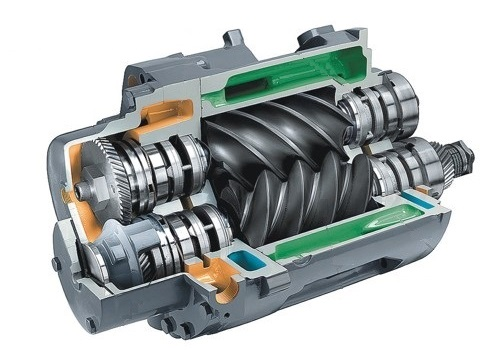
\includegraphics[width=0.6\linewidth]{Figuras/Ch01/fig1.jpg}}
	\begin{block}{Motivação}
		Como estão associados os resistores no circuito acima? Em série ou em paralelo? Como encontrar a \textbf{resistência equivalente} desse circuito?
	\end{block}
}

\frame{
	\frametitle{Rede estrela ($Y$)}
	
	\begin{minipage}{0.49\linewidth}
		\centering
		\begin{circuitikz}
			\draw (0,0) to[R,l_=$ R_1 $, o-*] ++(-30:1)
			to[R,l_=$ R_2 $, -o] ++(30:1) ++(30:-1)
			to[R=$ R_3 $, -*] ++(0,-1) ++(-0.5,0) to[short, o-o] ++(1,0);
		\end{circuitikz}\tikzmark{p1}
	\end{minipage}
	\hfill
	\begin{minipage}{0.49\linewidth}
		\centering
		\begin{circuitikz}
			\draw (0,0) to[R=$ R_1 $, o-*] ++(1,0)
			to[R=$ R_2 $, -o] ++(1,0) ++(-1,0)
			to[R=$ R_3 $] ++(0,-1) ++(-0.5,0) to[short, o-o] ++(1,0);
		\end{circuitikz}
	\end{minipage}

	\begin{tikzpicture}[remember picture, overlay]
		\draw[Implies-Implies, double distance=0.2cm,thick] (p1) ++(0,1.6cm) -- +(1,0);
	\end{tikzpicture}
	
%	\centerline{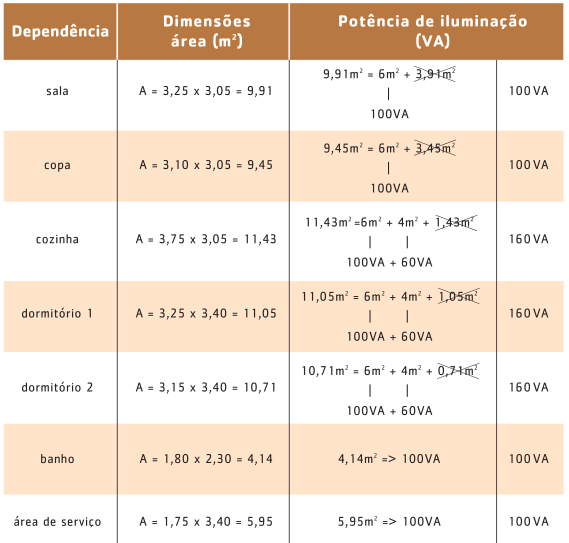
\includegraphics[width=0.9\linewidth]{Figuras/Ch01/fig2.png}}
}

\frame{
	\frametitle{Rede triângulo ($\Delta$)}
	
	\begin{minipage}{0.49\linewidth}
		\centering
		\begin{circuitikz}
			\draw (0.25,0) node[coordinate,name=a] {} ++(-30:1) node[coordinate,name=center] {}
			++(30:1) node[coordinate,name=b] {} ++(30:-1)
			++(0,-1) node[coordinate,name=c] {};
			\draw (0,0) to[short,o-] (a) to[R=$ R_c $] (b) to[short,-o] ++(0.25,0) (b)
			to[R,l^=$ R_a $, *-*] (c) (a)
			to[R,l_=$ R_b $, *-] (c) ++(-0.5,0) to[short, o-o] ++(1,0);
		\end{circuitikz}\tikzmark{p1}
	\end{minipage}
	\hfill
	\begin{minipage}{0.49\linewidth}
		\centering
		\begin{circuitikz}
			\draw (0.25,0) node[coordinate,name=a] {} ++(-30:1) node[coordinate,name=center] {}
			++(30:1) node[coordinate,name=b] {} ++(30:-1)
			++(0,-1) node[coordinate,name=c] {};
			\draw (0,0) to[short,o-] (a) to[R=$ R_c $] (b) to[short,-o] ++(0.25,0) (b)
			to[R,l^=$ R_a $, *-*] (b|-c) (a)
			to[R,l_=$ R_b $, *-*] (a|-c) ++(-0.25,0) to[short, o-o] ($ (b|-c)+(0.25,0) $);
		\end{circuitikz}
	\end{minipage}
	
	\begin{tikzpicture}[remember picture, overlay]
	\draw[Implies-Implies, double distance=0.15cm,thick] (p1) ++(-0.3,1.3cm) -- +(0.8,0);
	\end{tikzpicture}
	
%	\centerline{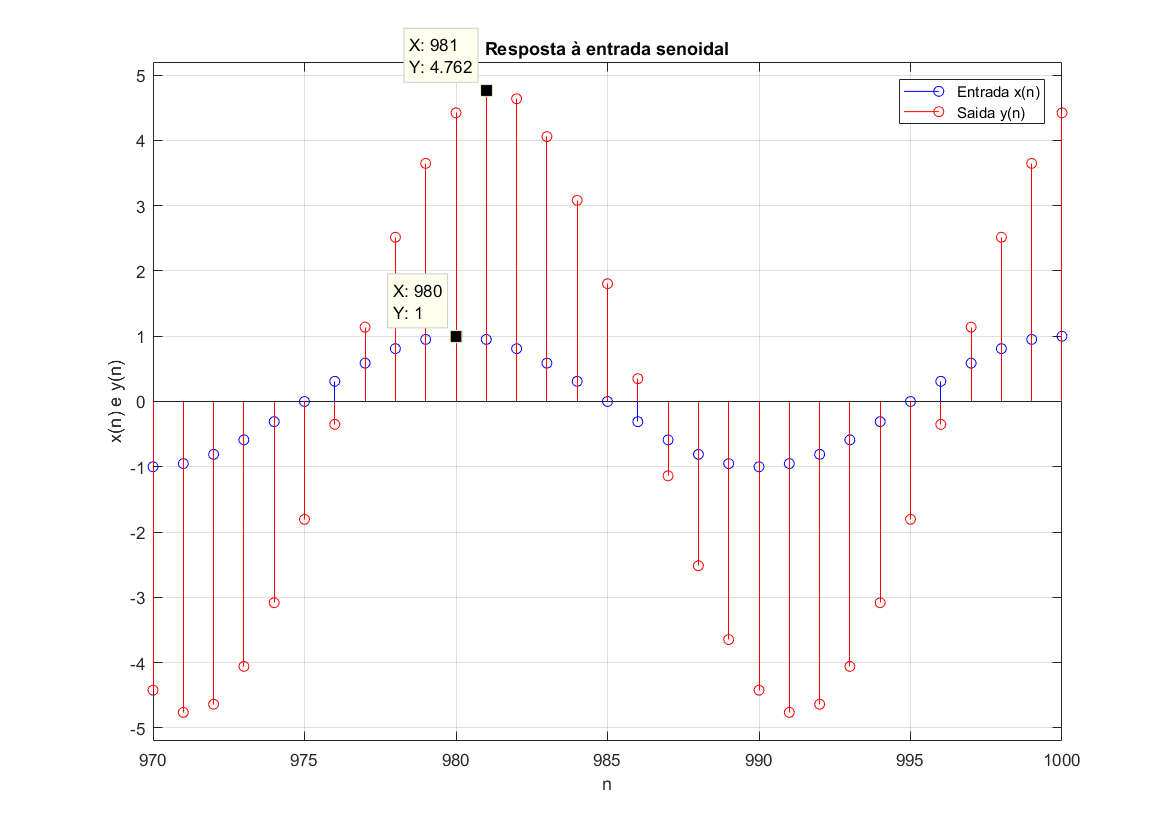
\includegraphics[width=0.9\linewidth]{Figuras/Ch01/fig3.png}}
}

\frame{
	\frametitle{Conversão $Y-\Delta$}
	\centering
	\begin{circuitikz}
		\draw[color=red] (0,0) node[coordinate,name=a] {} to[R,l_=$ R_1 $, o-*] ++(-30:1.5) node[coordinate,name=center] {}
		to[R,l_=$ R_2 $, -o] ++(30:1.5) node[coordinate,name=b] {} ++(30:-1.5)
		to[R=$ R_3 $, -*] ++(0,-1.5) node[coordinate,name=c] {} ++(-0.75,0);
		\draw[color=blue] (0,0) -- (a) to[R=$ R_c $, o-o] (b)
		to[R,l^=$ R_a $, *-*] (c) (a)
		to[R,l_=$ R_b $, *-] (c);
	\end{circuitikz}

	\begin{block}{Superposição}
		Observe o modelo de superposição das duas estruturas. Esse modelo ajuda a identificar a \textbf{conversão de uma rede para a outra}.
	\end{block}
}

\frame{
	\frametitle{Conversão $Y-\Delta$}
	\begin{block}{Terminais $1,3$}
		\textbf{Para o circuito em triângulo:}
		
		$$R_{1,3} = R_b \parallel (R_a + R_c) = \dfrac{R_b \cdot (R_a + R_c)}{R_b + R_a + R_c}$$
		
		\vspace{0.5cm}
		
		\textbf{Para o circuito em estrela:}
		
		$$R_{1,3} = R_1 + R_3$$
	\end{block}
}

\frame{
	\frametitle{Conversão $Y-\Delta$}
	\begin{block}{Terminais $1,2$}
		\textbf{Para o circuito em triângulo:}
		
		$$R_{1,2} = R_c \parallel (R_a + R_b) = \dfrac{R_c \cdot (R_a + R_b)}{R_c + R_a + R_b}$$
		
		\vspace{0.5cm}
		
		\textbf{Para o circuito em estrela:}
		
		$$R_{1,2} = R_1 + R_2$$
	\end{block}
}

\frame{
	\frametitle{Conversão $Y-\Delta$}
	\begin{block}{Terminais $2,4$}
		\textbf{Para o circuito em triângulo:}
		
		$$R_{2,4} = R_a \parallel (R_b + R_c) = \dfrac{R_a \cdot (R_b + R_c)}{R_a + R_b + R_c}$$
		
		\vspace{0.5cm}
		
		\textbf{Para o circuito em estrela:}
		
		$$R_{2,4} = R_2 + R_3$$
	\end{block}
}

\frame{
	\frametitle{Conversão $Y-\Delta$}
	\begin{block}{Importante}
		\begin{itemize}
			\item Quando sobrepomos um circuito em estrela a um circuito em triângulo, a resistência equivalente entre os terminais \textbf{deverá ser a mesma tanto para estrela, quanto para triângulo}. Deste modo:
		\end{itemize}
	
		\begin{gather}
		R_1 + R_3 = \dfrac{R_b \cdot (R_a + R_c)}{R_b + R_a + R_c} \label{eqn:1}\\
		R_1 + R_2 = \dfrac{R_c \cdot (R_a + R_b)}{R_c + R_a + R_b} \label{eqn:2}\\
		R_2 + R_3 = \dfrac{R_a \cdot (R_b + R_c)}{R_a + R_b + R_c} \label{eqn:3}
		\end{gather}

	\end{block}
}

\frame{
	\frametitle{Conversão $Y-\Delta$}
	\begin{block}{Obtenção das fórmulas}
		Subtraindo a equação \ref{eqn:3} da equação \ref{eqn:1}, obtemos:
		
		\begin{align}
			(R_2 + R_3) - (R_1 + R_3) &= \dfrac{R_a \cdot (R_b + R_c)}{R_a + R_b + R_c} - \dfrac{R_b \cdot (R_a + R_c)}{R_b + R_a + R_c} \nonumber\\
			R_2 - R_1 &= \dfrac{R_a \cdot R_b + R_a \cdot R_c - R_b \cdot R_a - R_b \cdot R_c}{R_b + R_a + R_c} \nonumber\\
			R_2 - R_1 &= \dfrac{R_a \cdot R_c - R_b \cdot R_c}{R_b + R_a + R_c} \nonumber\\
			R_1 - R_2 &= \dfrac{R_c \cdot (R_b - R_a)}{R_b + R_a + R_c} \label{eqn:4}
		\end{align}

	\end{block}
}

\frame{
	\frametitle{Conversão $Y-\Delta$}
	\begin{block}{Obtenção das fórmulas}
		Somando a equação \ref{eqn:2} da equação \ref{eqn:4}, obtemos:

		\begin{align}
			2 \cdot R_1 &= \dfrac{R_c \cdot R_b - R_c \cdot R_a + R_c \cdot R_a + R_c \cdot R_b}{R_b + R_a + R_c} \nonumber\\
			\Aboxed{R_1 &= \dfrac{R_b \cdot R_c}{R_a + R_b + R_c}} \label{eqn:5}
		\end{align}
	\end{block}
}

\frame{
	\frametitle{Conversão $Y-\Delta$}
	\begin{block}{Obtenção das fórmulas}
		Subtraindo a equação \ref{eqn:4} da equação \ref{eqn:2}, obtemos:

		\begin{align}
			-2 \cdot R_2 &= \dfrac{R_c \cdot R_b - R_c \cdot R_a - R_c \cdot R_a - R_c \cdot R_b}{R_b + R_a + R_c}\nonumber\\
			\Aboxed{R_2 &= \dfrac{R_a \cdot R_c}{R_a + R_b + R_c}} \label{eqn:6}
		\end{align}
	\end{block}
}

\frame{
	\frametitle{Conversão $Y-\Delta$}
	\begin{block}{Obtenção das fórmulas}
		Subtraindo a equação \ref{eqn:5} da equação \ref{eqn:1}, obtemos:

		\begin{align}
			-R_3 &= \dfrac{R_c \cdot R_b - R_b \cdot R_a - R_b \cdot R_c}{R_b + R_a + R_c}\nonumber\\
			\Aboxed{R_3 &= \dfrac{R_a \cdot R_b}{R_a + R_b + R_c}} \label{eqn:7}
		\end{align}
	\end{block}
}

\frame{
	\frametitle{Conversão $Y-\Delta$}
	\begin{block}{Regra Geral}
		Cada resistor do circuito em estrela é o \textbf{produto dos resistores nos dois ramos adjacentes} do circuito em triângulo, \textbf{dividido pela soma dos três resistores} em triângulo.
	\end{block}
}

\frame{
	\frametitle{Exemplo de Conversão $Y-\Delta$}
	
	\centering
	\begin{circuitikz}[scale=0.5]
		\draw (0,0) node[above] {$ A $} to[R=20<\ohm>,*-*] +(-60:2) node[below] {$ B $}
		to[R=12<\ohm>] (60:-2) node[below] {$ C $}
		to[R=68<\ohm>, *-] +(60:2);
	\end{circuitikz}
	
%	\centerline{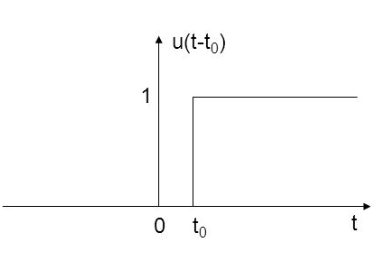
\includegraphics[width=0.3\linewidth]{Figuras/Ch01/fig5.PNG}}
	\begin{block}{Resolução}
		Resistores da rede $\Delta: R_a = 20 \si{\ohm}, R_b = 68 \si{\ohm}, R_c = \SI{12}{\ohm}$
		$$R_1 = \dfrac{R_b \cdot R_c}{R_a + R_b + R_c} = \dfrac{68 \cdot 12}{20 + 68 + 12} = \SI{8.16}{\ohm}$$
		$$R_2 = \dfrac{R_a \cdot R_c}{R_a + R_b + R_c} = \dfrac{20 \cdot 12}{20 + 68 + 12} = \SI{2.4}{\ohm}$$
		$$R_3 = \dfrac{R_a \cdot R_b}{R_a + R_b + R_c} = \dfrac{20 \cdot 68}{20 + 68 + 12} = \SI{13.6}{\ohm}$$
	\end{block}
}

\frame{
	\frametitle{Conversão $Y-\Delta$}
	\centering
	\begin{circuitikz}
		\draw[color=red] (0,0) node[coordinate,name=a] {} to[R,l_=$ R_1 $, o-*] ++(-30:1.5) node[coordinate,name=center] {}
		to[R,l_=$ R_2 $, -o] ++(30:1.5) node[coordinate,name=b] {} ++(30:-1.5)
		to[R=$ R_3 $, -*] ++(0,-1.5) node[coordinate,name=c] {} ++(-0.75,0);
		\draw[color=blue] (0,0) -- (a) to[R=$ R_c $, o-o] (b)
		to[R,l^=$ R_a $, *-*] (c) (a)
		to[R,l_=$ R_b $, *-] (c);
	\end{circuitikz}
%	\centerline{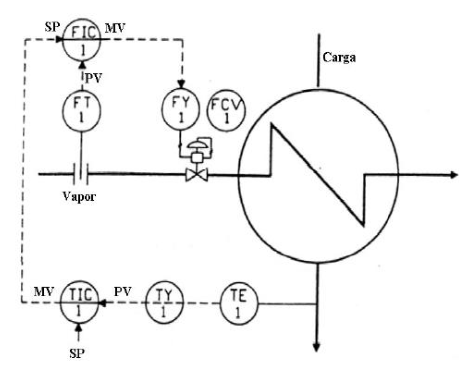
\includegraphics[width=0.5\linewidth]{Figuras/Ch01/fig4.png}}
	\begin{block}{Análogo}
		O princípio opara essa conversão é o mesmo para o circuito $\Delta-Y$, o que muda são as manipulações algébricas das equações.
	\end{block}
}

\frame{
	\frametitle{Conversão $Y-\Delta$}
	\begin{block}{Regra Geral}
		Cada resistor do circuito em triângulo é a \textbf{soma de todos os produtos possíveis dos resistores} do circuito em estrela tomados dois a dois, \textbf{dividido pelo resistor $\bm{Y}$ oposto}.

		\begin{equation*}
			\boxed{R_a = \dfrac{R_1 \cdot R_2 + R_1 \cdot R_3 + R_2 \cdot R_3}{R_1}}
		\end{equation*}
		\vspace{0.3cm}
		\begin{equation*}
			\boxed{R_b = \dfrac{R_1 \cdot R_2 + R_1 \cdot R_3 + R_2 \cdot R_3}{R_2}}
		\end{equation*}
		\vspace{0.3cm}
		\begin{equation*}
			\boxed{R_c = \dfrac{R_1 \cdot R_2 + R_1 \cdot R_3 + R_2 \cdot R_3}{R_3}}
		\end{equation*}
	\end{block}
}

\frame{
	\frametitle{Exemplo de Conversão $Y-\Delta$}
	
	\centering
	\begin{circuitikz}[scale=0.6, myR/.style = {R, resistors/scale=0.75, resistors/width=0.6, resistors/zigs=4}]
		\draw (0,0) node[above] {$ A $} to[myR,l=13.6<\ohm>, o-] ++(0,-1)
		to[myR,l_=8.16<\ohm>, *-o] ++(45:-1) node[below] {C} ++(45:1)
		to[myR,l=2.4<\ohm>, -o] ++(-45:1) node[below] {B};
	\end{circuitikz}
	
%	\centerline{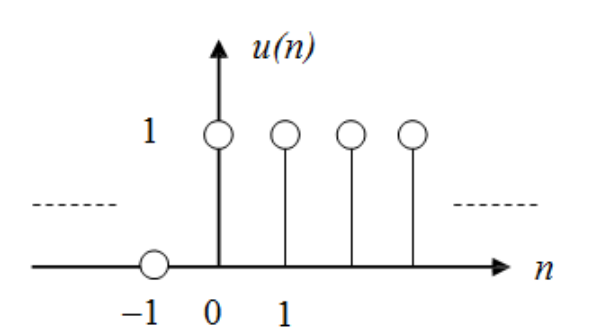
\includegraphics[width=0.22\linewidth]{Figuras/Ch01/fig6.PNG}}
	\begin{block}{Resolução}
		Resistores da rede $Y: R_1 = \SI{8.16}{\ohm}, R_2 = \SI{2.4}{\ohm}, R_3 = \SI{13.6}{\ohm}$
		$$R_a = \dfrac{R_1 \cdot R_2 + R_1 \cdot R_3 + R_2 \cdot R_3}{R_1} = \dfrac{\num{163,2}}{\num{8,16}} = \SI{20}{\ohm}$$
		$$R_b = \dfrac{R_1 \cdot R_2 + R_1 \cdot R_3 + R_2 \cdot R_3}{R_2} = \dfrac{\num{163,2}}{\num{2,4}} = \SI{68}{\ohm}$$
		$$R_c = \dfrac{R_1 \cdot R_2 + R_1 \cdot R_3 + R_2 \cdot R_3}{R_3} = \dfrac{\num{163,2}}{\num{13,6}} = \SI{12}{\ohm}$$
	\end{block}
}

\frame{
	\frametitle{Observação}
	\begin{block}{Rede equilibrada}
		As redes $Y$ e $\Delta$ são equilibradas quando:
		$$R_1 = R_2 = R_3 = R_Y \hspace{1.5cm} R_a = R_b = R_c = R_{\Delta}$$
		
		Logo,
		$$\boxed{R_Y = \dfrac{R_{\Delta}}{3}}$$
	\end{block}
}

\section*{Exercícios}
\frame{
	\frametitle{Exercícios}
	\begin{block}{}
		01. Encontre a resistência equivalente do circuito abaixo utilizando a transformação estrela-triângulo.
		
		\vspace{0.5cm}
		
		\centerline{\includegraphics[width=0.6\linewidth]{Figuras/Ch01/fig7.PNG}}
	\end{block}
}

\section*{Referências}

\frame{
	\frametitle{Referências e Exercícios Complementares}
	\begin{itemize}
		\item ALEXANDRE, Charles K.; SADIKU, Matthew N. O. Fundamentos de Circuitos Elétricos. 5. ed. Porto Alegre: AMGH, 2013.
	\end{itemize}
	%\centering{\alert{Página 36 - \textbf{1.6.1 até 1.6.5, 1.6.17 até 1.6.19}}} \\
	\centering{\alert{Lista de exercícios 01}}
}
%\section{Conceitos Gerais. LKC e LKT}

\frame{
	\frametitle{Introdução}
	\begin{block}{Contextualização}
		Um circuito elétrico pode ser composto por várias malhas, constituídas por elementos que geram ou absorvem energia elétrica. Para calcular as tensões e correntes nesses elementos, necessitamos utilizar as Leis de Kirchhoff devido à complexidade do circuito. Para utilizar estas Leis, precisamos destacar trechos nos quais se aplicam propriedades, facilitando o equacionamento.
	\end{block}
}

\frame{
	\frametitle{Conceitos gerais para análise de circuitos}
	\centerline{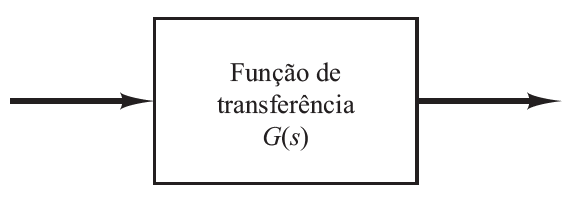
\includegraphics[width=0.5\linewidth]{Figuras/Ch02/fig1.PNG}}
	\begin{block}{Nó}
		Num circuito um \textbf{nó} é qualquer ponto do circuito em que \textbf{três ou mais terminais se liguem}.
		
		\textbf{Obs.:} Alguns autores definem nó como a conexão de \textbf{dois ou mais terminais}. \\
		\begin{itemize}
			\item Neste exemplo, os pontos $B$ e $E$ formam dois nós, em que se interligam geradores e resistores.
		\end{itemize}
	\end{block}
}

\frame{
	\frametitle{Conceitos gerais para análise de circuitos}
	\centerline{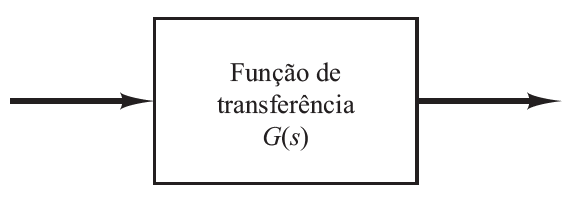
\includegraphics[width=0.5\linewidth]{Figuras/Ch02/fig1.PNG}}
	\begin{block}{Ramo}
		O \textbf{ramo} é o único caminho entre dois nós consecutivos. \\
		\begin{itemize}
			\item Neste exemplo, temos três ramos distintos: o ramo à esquerda composto por $E_6$, $R_1$, $E_1$ e $E_2$, o ramo central composto por $E_3$ e $R_2$ e o ramo à direita, composto por $R_5$, $E_5$, $R_4$, $E_4$ e $R_3$.
		\end{itemize}
	\end{block}
}

\frame{
	\frametitle{Conceitos gerais para análise de circuitos}
	\centerline{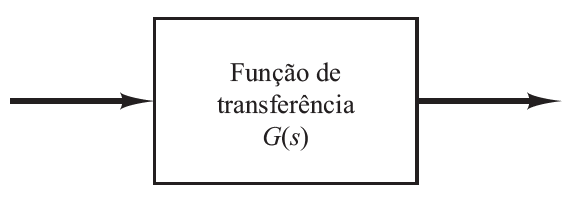
\includegraphics[width=0.5\linewidth]{Figuras/Ch02/fig1.PNG}}
	\begin{block}{Malha}
		Definimos \textbf{malha} como sendo todo circuito fechado constituído por elementos elétricos. \\
		\begin{itemize}
			\item Neste exemplo, notamos que o circuito é composto por três malhas: $ABEF$, $BCDE$ e $ABCDEF$, sendo esta última denominada malha externa.
		\end{itemize}
	\end{block}
}

\frame{
	\frametitle{Leis de Kirchhoff}
	\begin{block}{Introdução}
		A \textbf{Lei de Ohm} por si só não é suficiente para analisar \textbf{circuitos multi-malhas}. Quando unida com as \textbf{Leis de Kirchhoff} formam uma ferramenta poderosa na análise dos circuitos elétricos.
	\end{block}
}

\frame{
	\frametitle{Leis de Kirchhoff}
	\begin{block}{As Leis}
		\begin{enumerate}
			\item 1ª Lei: \textbf{LKC} (Lei de Kirchhoff para Correntes) ou lei dos nós.
			\item 2ª Lei: \textbf{LKT} (Lei de Kirchhoff para Tensões) ou lei das malhas.
		\end{enumerate}
	\end{block}
}

\frame{
	\frametitle{Leis de Kirchhoff - LKC}
	\centerline{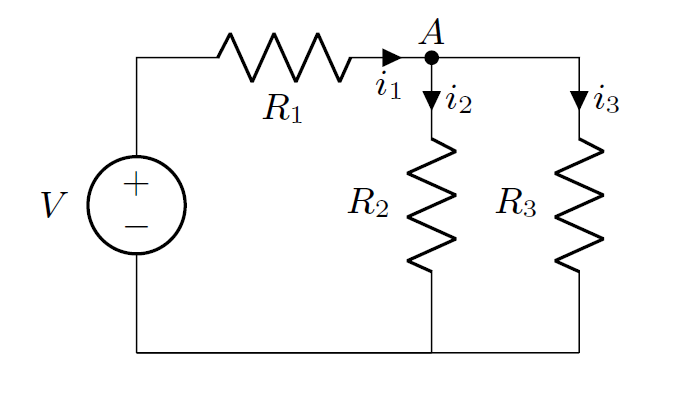
\includegraphics[width=0.6\linewidth]{Figuras/Ch02/fig2.PNG}}
	\begin{block}{Contextualização}
		No nó $A$ entra a corrente total do circuito e do mesmo nó partem as correntes parciais para cada resistor. Como no nó não há possibilidade de armazenamento de cargas ou vazamento das mesmas, tem-se que a \textbf{quantidade de cargas que chegam ao nó é exatamente igual à quantidade de cargas que saem do nó}.
	\end{block}
}

\frame{
	\frametitle{Leis de Kirchhoff - LKC}
	\centerline{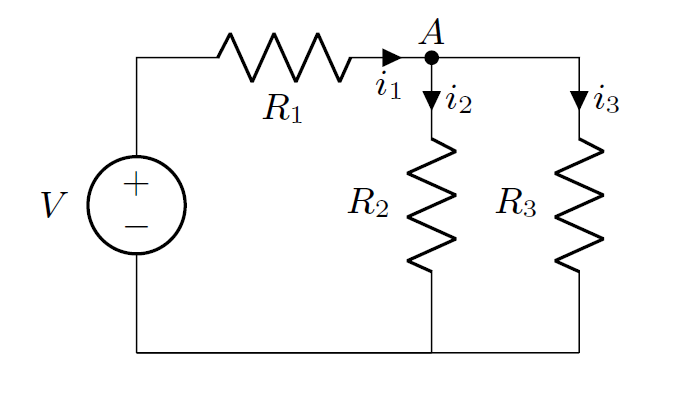
\includegraphics[width=0.6\linewidth]{Figuras/Ch02/fig2.PNG}}
	\begin{block}{Enunciado da 1a Lei de Kirchhoff}
		\textbf{``A soma das correntes que chegam em um nó é sempre igual à soma das correntes que saem deste nó."}
		$$\boxed{\sum_{i=1}^{n} I_{i_{\text{chegam}}} = \sum_{j=1}^{m} I_{j_{\text{saem}}}}$$
	\end{block}
}

\frame{
	\frametitle{Leis de Kirchhoff - LKC}
	\centerline{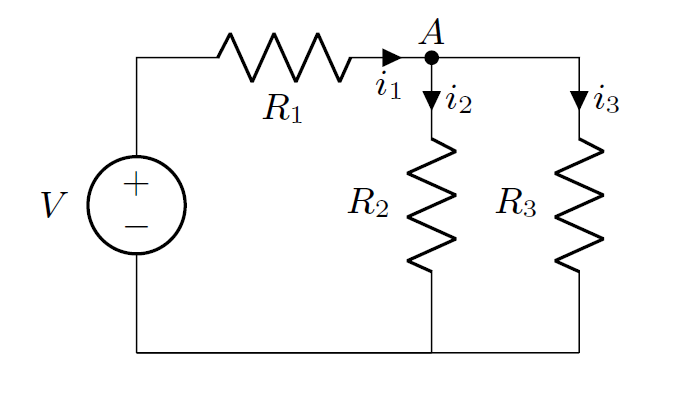
\includegraphics[width=0.5\linewidth]{Figuras/Ch02/fig2.PNG}}
	\begin{block}{Enunciado da 1a Lei de Kirchhoff - alternativo}
		\textbf{``A soma algébrica das correntes que entram e saem de um nó é nula"}. Consideramos que as correntes que \textbf{entram} no nó são \textbf{positivas}, e as que \textbf{saem} são \textbf{negativas}.
		$$\boxed{\sum_{i=1}^{n} I_{i} = 0}$$
	\end{block}
}

\frame{
	\frametitle{Leis de Kirchhoff - LKC}
	\centerline{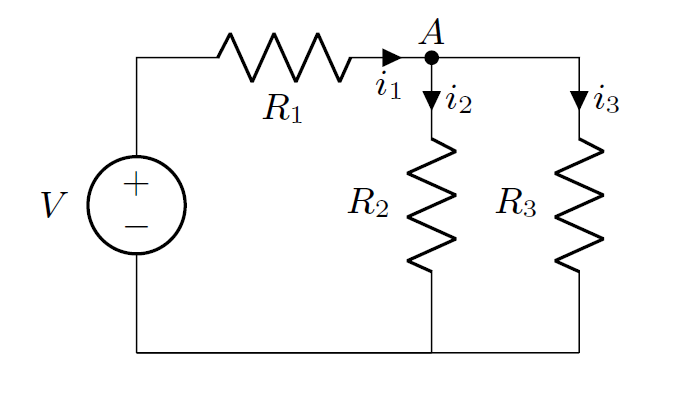
\includegraphics[width=0.6\linewidth]{Figuras/Ch02/fig2.PNG}}
	\begin{block}{Resolução}
		Primeira análise: $i_1 = i_2 + i_3$ \\
		Segunda análise: $i_1 - i_2 - i_3 = 0$ \\
		\begin{itemize}
			\item \textbf{Independente da abordagem escolhida, os resultados são equivalentes}.
		\end{itemize}
	\end{block}
}

\frame{
	\frametitle{Leis de Kirchhoff - LKT}
	\centerline{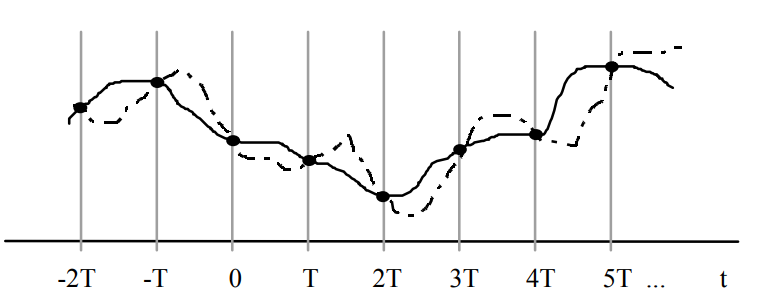
\includegraphics[width=0.7\linewidth]{Figuras/Ch02/fig3.PNG}}
	\begin{block}{Contextualização}
		A lei de Kirchhoff das tensões é aplicada nas malhas. Ela já foi usada no estudo dos
		circuitos de \textbf{resistores em série}, onde a soma das quedas de tensão nos resistores é igual à f.e.m. da fonte.
	\end{block}
}

\frame{
	\frametitle{Leis de Kirchhoff - LKT}
	\centerline{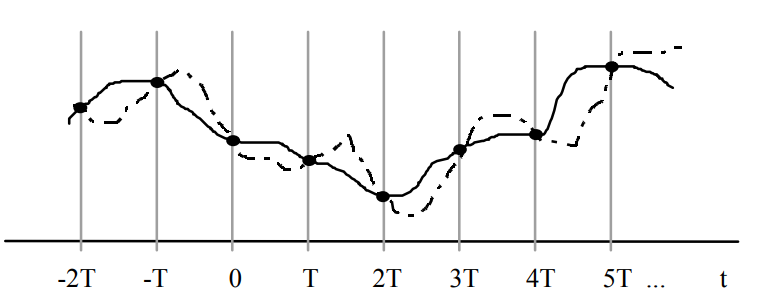
\includegraphics[width=0.6\linewidth]{Figuras/Ch02/fig3.PNG}}
	\begin{block}{Enunciado da 2a Lei de Kirchhoff}
		\textbf{``Em um percurso fechado, a soma algébrica das elevações de tensão é igual a soma algébrica das quedas de tensão."}
		$$\boxed{\sum_{i=1}^{n} V_{i_{\text{elevação}}} = \sum_{j=1}^{m} V_{j_{\text{queda}}}}$$
	\end{block}
}

\frame{
	\frametitle{Leis de Kirchhoff - LKT}
	\vspace{-0.3cm}
	\centerline{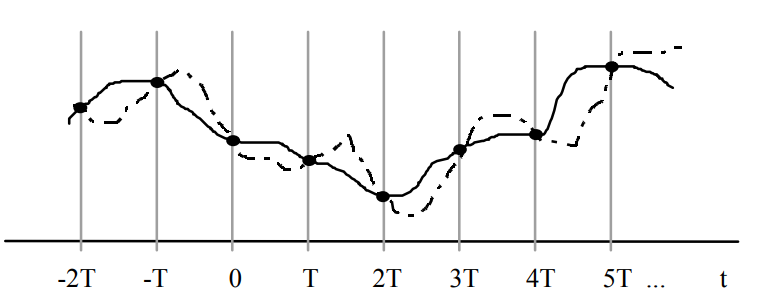
\includegraphics[width=0.6\linewidth]{Figuras/Ch02/fig3.PNG}}
	\begin{block}{Enunciado da 2a Lei de Kirchhoff - alternativo}
		\textbf{``A soma algébrica de todas as tensões em torno de um caminho fechado (ou malha) é zero"}. Consideramos que as \textbf{elevações} de tensão são \textbf{positivas} e as \textbf{quedas} de tensão são \textbf{negativas}.
		$$\boxed{\sum_{i=1}^{n} V_{i} = 0}$$
	\end{block}
}

\frame{
	\frametitle{Leis de Kirchhoff - LKT}
	\vspace{-0.3cm}
	\centerline{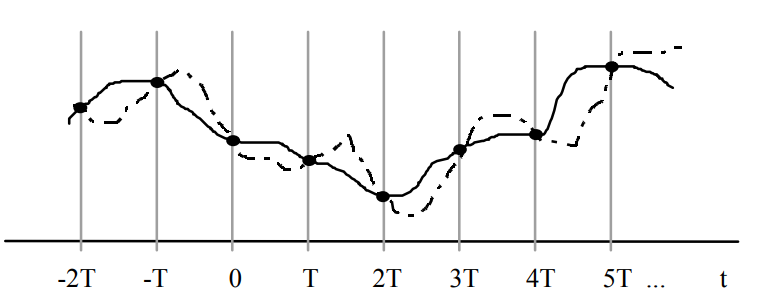
\includegraphics[width=0.7\linewidth]{Figuras/Ch02/fig3.PNG}}
	\begin{block}{Resolução - sentido horário da corrente}
		Primeira análise: $V_4 + V_5 = V_1 + V_2 + V_3$ \\
		Segunda análise: $V_4 - V_1 - V_2 + V_5 - V_3 = 0$ \\
		\begin{itemize}
			\item \textbf{Independente da abordagem escolhida, os resultados são equivalentes}.
		\end{itemize}
	\end{block}
}

\frame{
	\frametitle{Leis de Kirchhoff - LKT}
	\vspace{-0.3cm}
	\centerline{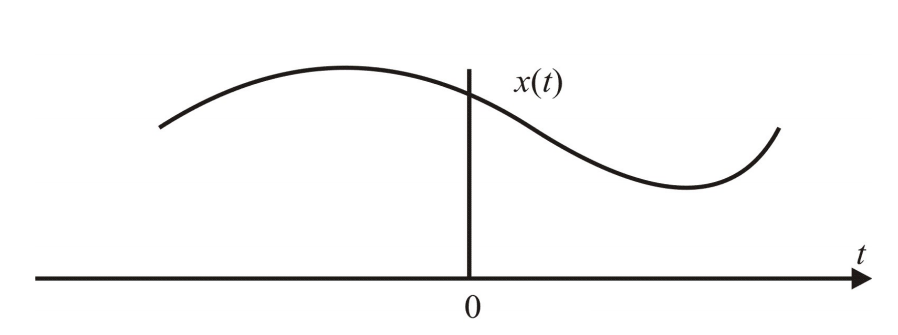
\includegraphics[width=0.7\linewidth]{Figuras/Ch02/fig4.PNG}}
	\begin{block}{Resolução - sentido anti-horário da corrente}
		Primeira análise: $V_2 + V_1 + V_3 = V_4 + V_5$ \\
		Segunda análise: $V_1 - V_4 + V_3 - V_5 + V_2 = 0$ \\
		\begin{itemize}
			\item \textbf{Independente da abordagem escolhida, os resultados são equivalentes}.
		\end{itemize}
	\end{block}
}

\section*{Exercícios}
\frame{
	\frametitle{Exercícios}
	\begin{block}{}
		01. Encontre $i_3$, $i_4$, $i_6$ e $i_7$.
		\vspace{0.1cm}
		\centerline{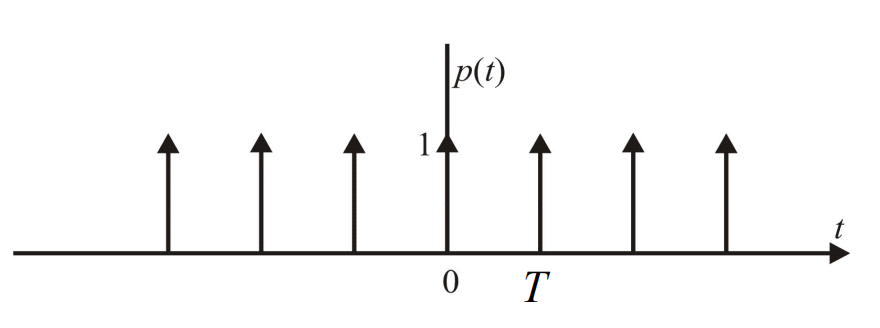
\includegraphics[width=0.9\linewidth]{Figuras/Ch02/fig5.PNG}}
	\end{block}
}

\section*{Exercícios}
\frame{
	\frametitle{Exercícios}
	\begin{block}{}
		02. Determine $V_1$ e $V_2$ no circuito abaixo.
		\centerline{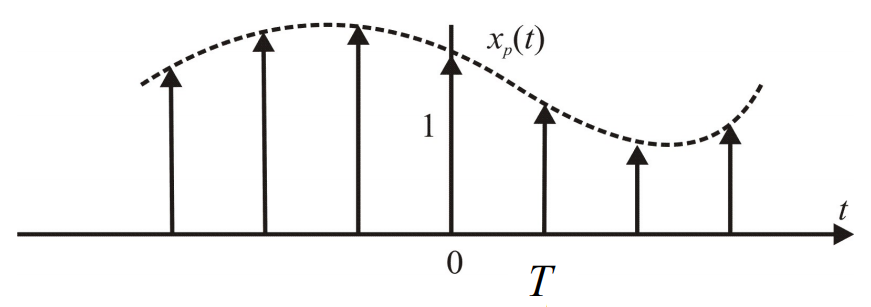
\includegraphics[width=0.8\linewidth]{Figuras/Ch02/fig6.PNG}}
	\end{block}
}

\section*{Referências}

\frame{
	\frametitle{Referências e Exercícios Complementares}
	\begin{itemize}
		\item ALEXANDRE, Charles K.; SADIKU, Matthew N. O. Fundamentos de Circuitos Elétricos. 5. ed. Porto Alegre: AMGH, 2013.
	\end{itemize}
	%\centering{\alert{Página 36 - \textbf{1.6.1 até 1.6.5, 1.6.17 até 1.6.19}}} \\
	\centering{\alert{Lista de exercícios 02}}
}




%%%%%%%%%%%%%%%%%%%%%%%%%%%%%%%%%%%%%%%%%%%%
%%%%%%%%%%%%%%%%%%%%%%%%%%%%%%%%%%%%%%%%%%%
%%%%%%%%%%%%%%% CHAPTER 03 %%%%%%%%%%%%%%%%


\section{Sensoriamento e atuadores}

\frame{
\frametitle{Sensores}
\begin{block}{Contextualização}
O velocímetro de um automóvel indica a velocidade de deslocamento porque existe um \textbf{sensor} que é capaz de medir a velocidade das rodas.
\end{block}
\centerline{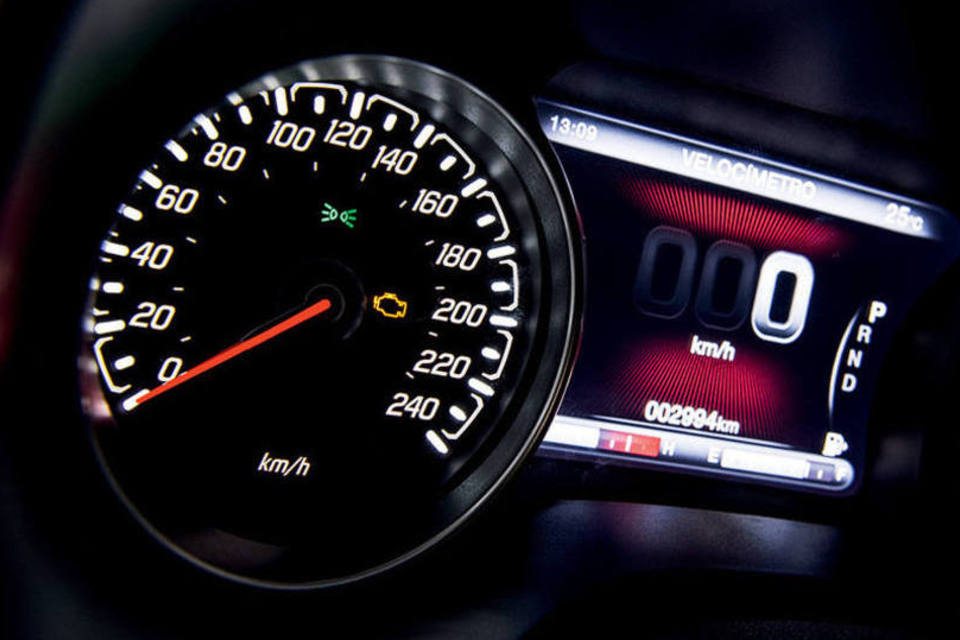
\includegraphics[width=0.7\linewidth]{Figuras/Ch03/fig1.jpeg}}
}

\frame{
\frametitle{Sensores}
\begin{block}{Contextualização}
A porta de uma geladeira ao ser
aberta acende a luz, porque há um \textbf{sensor} que indica que ela foi aberta.
\end{block}
\centerline{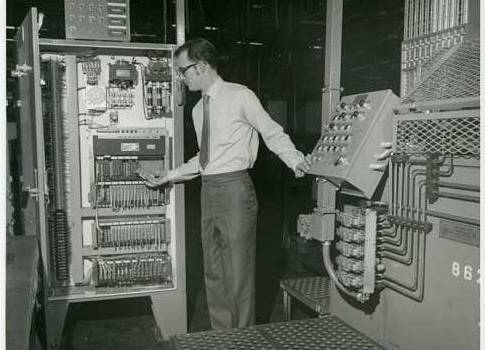
\includegraphics[width=0.3\linewidth]{Figuras/Ch03/fig2.jpg}}
}

\frame{
\frametitle{Sensores}
\centerline{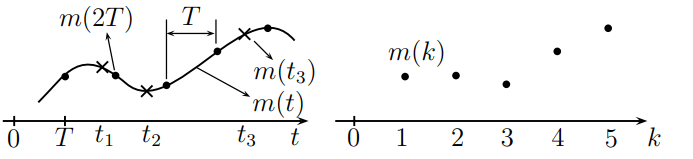
\includegraphics[width=0.9\linewidth]{Figuras/Ch03/fig3.PNG}}
\begin{block}{Definição}
É um dispositivo capaz de \textbf{monitorar a variação de uma grandeza física} e transmitir esta informação a um sistema em que a indicação seja inteligível para nós ou para o elemento de controle do sistema.
\end{block}
}

\frame{
\frametitle{Transdutores}
\begin{block}{Definição}
Todos os dispositivos sensores são compostos por elementos denominados \textbf{transdutores}, pois são capazes de \textbf{transformar um tipo de energia em outro}. A maior parte dos sensores é constituída por transdutores que convertem uma grandeza de entrada em uma \textbf{grandeza elétrica}, que pode ser processada por um circuito elétrico ou eletrônico.
\begin{itemize}
    \item Transdutor: é todo dispositivo que recebe um sinal de entrada na forma de uma grandeza física, e fornece uma resposta na saída, da mesma espécie ou diferente, que reproduz certas características do sinal de entrada a partir de uma relação definida.
\end{itemize}
\end{block}
}

\frame{
\frametitle{Tipos de sinais}
\begin{block}{Definição}
\begin{itemize}
    \item Os sensores podem ser classificados segundo o \textbf{tipo de sinal} que transformam. Assim, para estudar sensores é necessário começar pelos tipos de sinais.
\end{itemize}
Um sinal é uma \textbf{informação} na forma de um valor (ou de uma curva de valores) de uma grandeza física.
\end{block}
}

\frame{
\frametitle{Tipos de sinais}
\begin{block}{Sinal digital}
\begin{itemize}
    \item O \textbf{sinal digital binário} só pode assumir \textbf{dois valores}. 
    \item Estes valores são associados a
    \textbf{estados} que podem indicar, por exemplo, se uma pressão está acima ou abaixo de uma determinada referência. 
    \item O valor 0 (\textbf{zero}) é geralmente utilizado para indicar estados como “falso”, “aberto”, “desligado” ou “abaixo da referência”.
    \item O valor 1 (\textbf{um}) pode
    indicar estados como “verdadeiro”, “fechado”, “ligado” ou “acima da referência”.
\end{itemize}
\end{block}
}

\frame{
\frametitle{Tipos de sinais}
\centerline{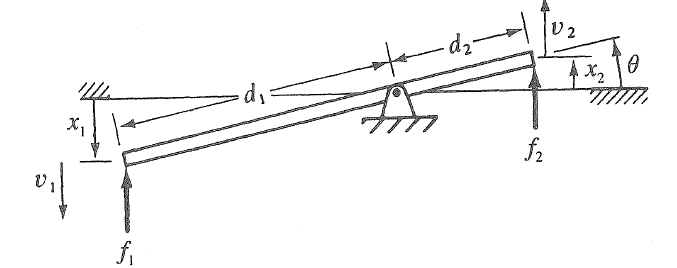
\includegraphics[width=0.6\linewidth]{Figuras/Ch03/fig4.PNG}}
}

\frame{
\frametitle{Tipos de sinais}
\centerline{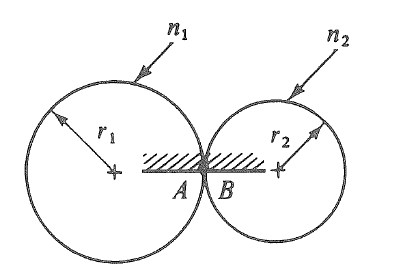
\includegraphics[width=1.1\linewidth]{Figuras/Ch03/fig5.PNG}}
}

\frame{
\frametitle{Tipos de sinais}
\begin{block}{Sinal analógico}
\begin{itemize}
    \item Um \textbf{sinal analógico} é um sinal
    \textbf{contínuo} que representa a evolução de uma grandeza, de uma variável e que apresenta \textbf{infinitos valores} mesmo que estes valores estejam em uma faixa determinada. 
    \item Vamos nos imaginar medindo o nível de um reservatório e que este nível pode variar de 0 a 10 metros de altura. Há infinitos valores de nível nesta faixa e um sinal analógico, por ser contínuo, pode representar todos estes valores. Por exemplo, o nível do reservatório pode ser de 2 metros, de 3,5 metros, de 9,75 metros, ou seja, qualquer valor entre 0 e 10 metros.
\end{itemize}
\end{block}
}

\frame{
\frametitle{Tipos de sinais}
\centerline{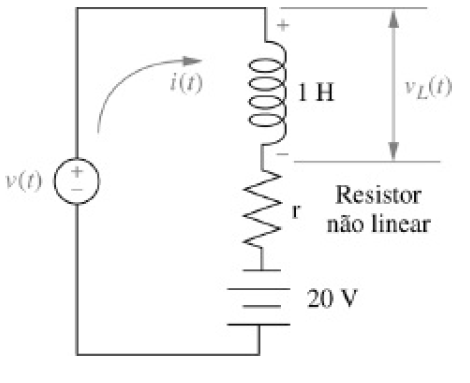
\includegraphics[width=0.6\linewidth]{Figuras/Ch03/fig6.PNG}}
}

\frame{
\frametitle{Tipos de sinais}
\centerline{\includegraphics[width=1.1\linewidth]{Figuras/Ch03/fig7.PNG}}
}

\frame{
\frametitle{Características}
\begin{block}{Linearidade}
Esse conceito se aplica a \textbf{sensores analógicos}. É a curva de saída do sensor a partir da grandeza medida. Buscam-se \textbf{respostas proporcionais às entradas} (lineares), para facilitar a montagem do circuito de interface, porém \textbf{nem sempre isso é possível}, pois alguns sensores não são lineares. 
\end{block}
\centerline{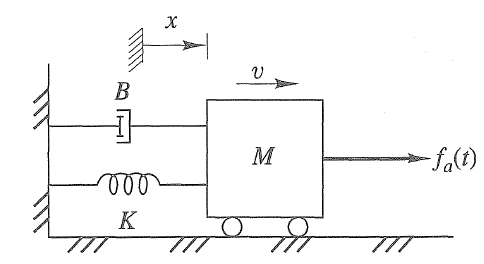
\includegraphics[width=1.1\linewidth]{Figuras/Ch03/fig8.PNG}}
}

\frame{
\frametitle{Características}
\begin{block}{Alcance (Range)}
Representa \textbf{toda a faixa de valores de entrada} de um sensor.
\end{block}
}

\frame{
\frametitle{Características}
\begin{block}{Velocidade de resposta}
Trata-se da \textbf{velocidade com que o sensor fornece o valor da variável}. O ideal é que o sensor possua uma resposta instantânea, pois uma resposta lenta pode prejudicar muito a eficiência do sistema de controle.
\end{block}
}

\frame{
\frametitle{Características}
\begin{block}{Repetibilidade}
É a habilidade do sensor de \textbf{detectar o
mesmo objeto à mesma distância, todas as vezes}.
Expresso como um percentual da distância sensora
nominal, esse número é baseado em uma temperatura ambiente constante e tensão da fonte.
\end{block}
}

\frame{
\frametitle{Sensores mecânicos}
\begin{block}{Chaves de fim de curso}
Uma chave fim de curso é um dispositivo
eletromecânico que consiste de um atuador
mecanicamente conectado a um conjunto de contatos. Podem determinar a presença ou ausência, passagem, posicionamento e término do curso de um objeto, por isso o nome de "chave fim de curso".
\end{block}
\centerline{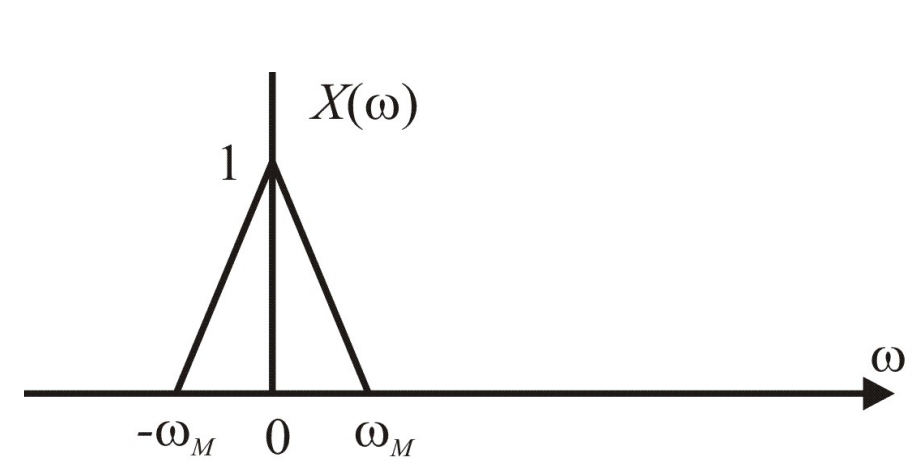
\includegraphics[width=0.9\linewidth]{Figuras/Ch03/fig9.PNG}}
}

\frame{
\frametitle{Sensores mecânicos}
\begin{block}{Chaves de fim de curso}
O tipo de sensor utilizado na porta da geladeira para acender e apagar a lâmpada é um detector de contato. 
\end{block}
\centerline{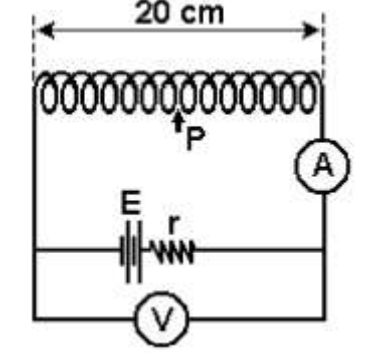
\includegraphics[width=0.5\linewidth]{Figuras/Ch03/fig10.PNG}}
}

\frame{
\frametitle{Sensores mecânicos}
\begin{block}{Chaves de fim de curso}
Outra aplicação possível é na \textbf{contagem e detecção de peças}.
\end{block}
\centerline{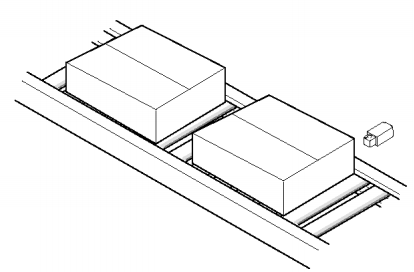
\includegraphics[width=0.7\linewidth]{Figuras/Ch03/fig11.PNG}}
}

\frame{
\frametitle{Sensores mecânicos}
\begin{block}{Chaves de fim de curso}
\textbf{Vantagens}:
\begin{itemize}
    \item Fácil utilização.
    \item Operação visível simples.
    \item Alta resistência para diferentes condições de ambiente.
    \item Alta repetibilidade.
\end{itemize}
\vspace{0.3cm}
\textbf{Desvantagens}:
\begin{itemize}
    \item Vida de contato mais curta do que as
    tecnologias de estado sólido.
    \item Peças mecânicas móveis podem apresentar desgaste.
    \item Nem todas as aplicações podem usar detecção por contato.
\end{itemize}
\end{block}
}

\frame{
\frametitle{Sensores mecânicos}
\begin{block}{Reed-Switch}
São chaves acionadas por \textbf{campo magnético}.
\end{block}
\centerline{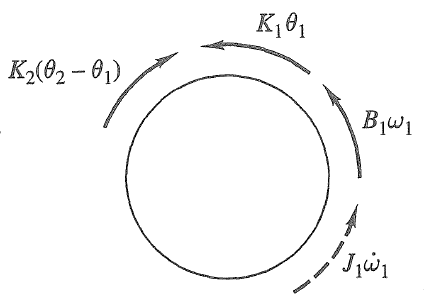
\includegraphics[width=0.9\linewidth]{Figuras/Ch03/fig12.PNG}}
}

\frame{
\frametitle{Sensores mecânicos}
\begin{block}{Reed-Switch}
Para proteger uma porta, uma janela ou um objeto qualquer contra a abertura ou remoção o que se faz é prender o ímã na parte móvel (porta, janela ou objeto) e o reed-switch na parte fixa (batente ou mesa).
\begin{itemize}
    \item O circuito deve ser projetado para operar no modo NF (Normalmente Fechado), ou seja, o circuito permanece desligado quando o reed-switch está fechado, ou com o ímã próximo.
    \item Quando o ímã é afastado, o reed-switch abre e com isso o circuito é ativado, disparando um \textbf{alarme} ou sistema de aviso.
\end{itemize}
\end{block}
\centerline{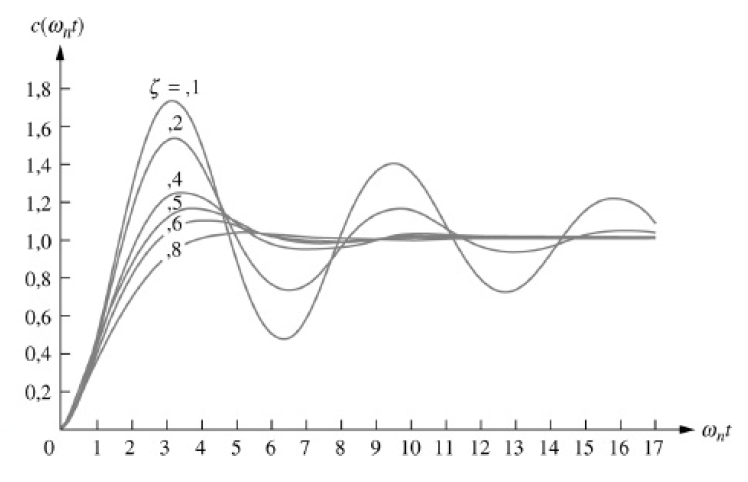
\includegraphics[width=0.5\linewidth]{Figuras/Ch03/fig13.PNG}}
}

\frame{
\frametitle{Sensores mecânicos}
\begin{block}{Reed-Switch}
\textbf{Vantagens}:
\begin{itemize}
    \item Fácil utilização.
    \item Barato.
    \item Alta velocidade de resposta.
\end{itemize}
\vspace{0.3cm}
\textbf{Desvantagens}:
\begin{itemize}
    \item Fragilidade mecânica.
    \item Susceptibilidade em gerar falso alarme.
    \item Consumo excessivo que reduz a vida útil da bateria.
\end{itemize}
\end{block}
}

\frame{
\frametitle{Sensores indutivos}
\begin{block}{}
Um sensor indutivo é usado para \textbf{detectar a presença de objetos metálicos}. O seu funcionamento é baseado, de acordo com sua característica física no \textbf{princípio da variação da indutância eletromagnética}. Ao energizar a bobina cria-se o campo eletromagnético.
\begin{itemize}
    \item Quando se introduz um objeto metálico na região ativa do sensor ocorre a detecção do objeto. Instantaneamente, o sinal da saída do sensor, que é um \textbf{sinal digital}, é modificado enviando a informação para o circuito ou para entrada digital de um equipamento que irá processá-la, como um CLP, por exemplo.
\end{itemize}
\end{block}
}

\frame{
\frametitle{Sensores indutivos}
\centerline{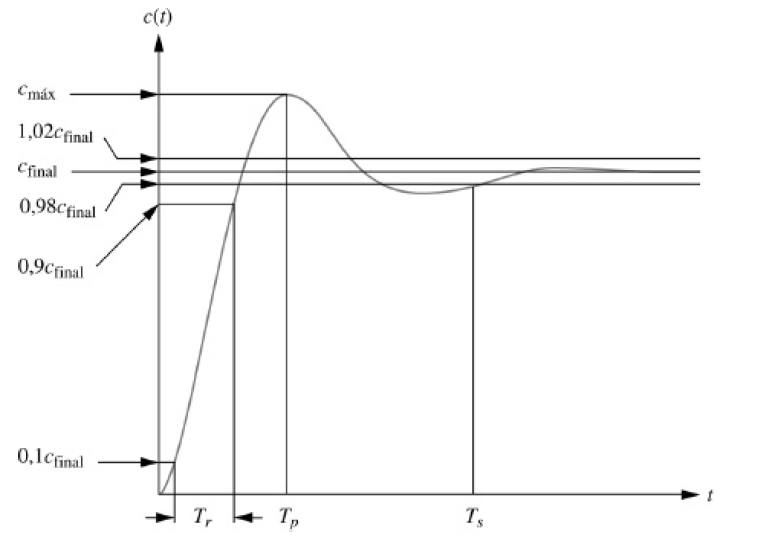
\includegraphics[width=0.8\linewidth]{Figuras/Ch03/fig14.PNG}}
}

\frame{
\frametitle{Sensores indutivos}
\begin{block}{}
\textbf{Vantagens}:
\begin{itemize}
    \item Não são afetados pela umidade.
    \item Não são afetados pelos ambientes com poeira/sujeira.
    \item Sem partes móveis/sem desgaste mecânico.
    \item Não dependem de cor.
\end{itemize}
\vspace{0.3cm}
\textbf{Desvantagens}:
\begin{itemize}
    \item Detectam somente a presença de alvos metálicos.
    \item Podem ser afetados por campos eletromagnéticos fortes.
\end{itemize}
\end{block}
}

\frame{
\frametitle{Sensores indutivos}
\centerline{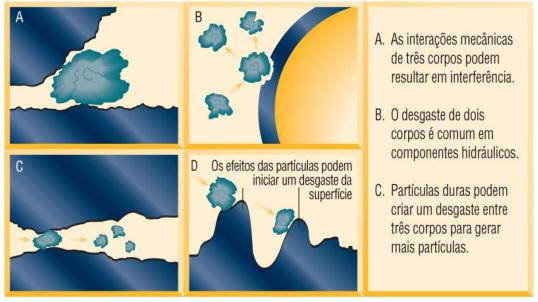
\includegraphics[width=0.9\linewidth]{Figuras/Ch03/fig15.jpg}}
}


\frame{
\frametitle{Sensores fotoelétricos}
\begin{block}{Introdução}
Sensores que trabalham com \textbf{luz} são muito mais rápidos que sensores mecânicos, pois não apresentam inércia e não tem peças móveis que quebram ou desgastam. \textbf{Os sensores fotoelétricos podem ser de diversos tipos}, sendo empregados numa infinidade de aplicações na indústria e em outros campos.
\end{block}
}

\frame{
\frametitle{Sensores fotoelétricos}
\begin{block}{LDR}
Os LDR’s possuem uma superfície de Cádmio (CdS) que tem sua \textbf{resistência elétrica dependente da quantidade de luz incidente}.
\end{block}
\vspace{0.2cm}
\centerline{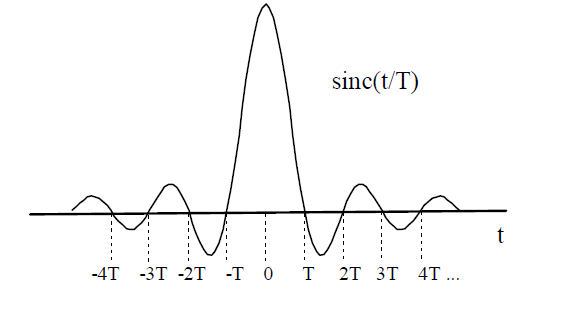
\includegraphics[width=0.9\linewidth]{Figuras/Ch03/fig16.PNG}}
}

\frame{
\frametitle{Sensores fotoelétricos}
\begin{block}{Curva característica do LDR}
A resistência elétrica do LDR decai à medida que a intensidade luminosa aumenta. 
\end{block}
\vspace{0.2cm}
\centerline{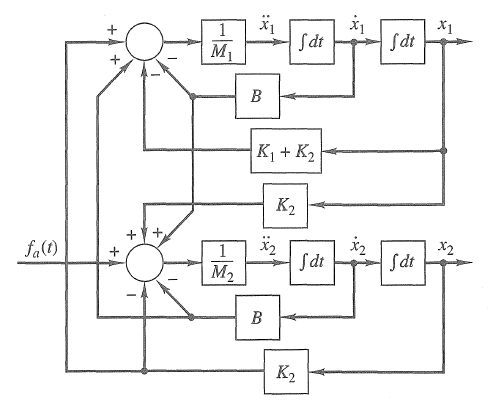
\includegraphics[width=0.6\linewidth]{Figuras/Ch03/fig17.PNG}}
}

\frame{
\frametitle{Sensores fotoelétricos}
\begin{block}{LDR}
\textbf{Vantagens}:
\begin{itemize}
    \item Podem operar com correntes relativamente altas, sendo muito sensíveis.
    \item Fácil utilização.
    \item Baixo preço.
\end{itemize}
\vspace{0.3cm}
\textbf{Desvantagem}:
\begin{itemize}
    \item Baixa velocidade de resposta - eles são sensores lentos.
\end{itemize}
\end{block}
}

\frame{
\frametitle{Sensores fotoelétricos}
\begin{block}{Fotocélula}
São dispositivos que geram uma pequena tensão elétrica quando são iluminados. As fotocélulas podem ser usadas para gerar energia elétrica a
partir da energia solar, ou também como sensores.
\end{block}
\vspace{0.2cm}
\centerline{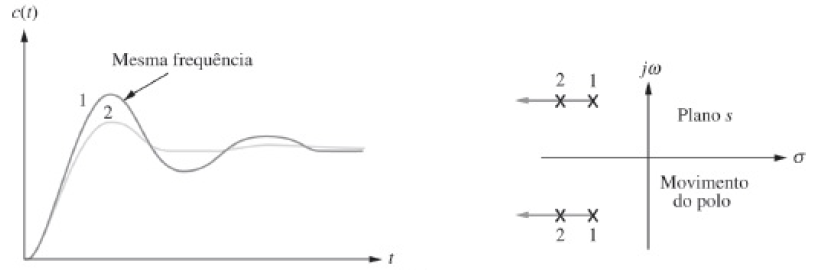
\includegraphics[width=0.3\linewidth]{Figuras/Ch03/fig18.PNG}}
}

\frame{
\frametitle{Sensores fotoelétricos}
\begin{block}{Fotocélula}
Uma aplicação possível é acionar o conjunto de iluminação de um estacionamento em função da diminuição da claridade do dia.
\end{block}
\vspace{0.2cm}
\centerline{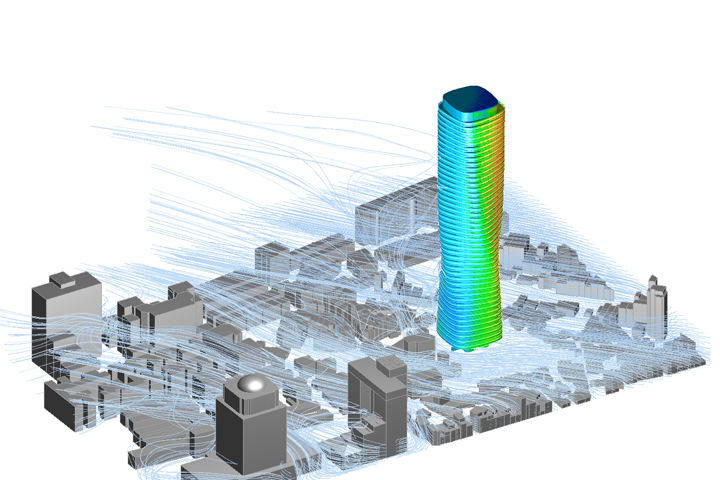
\includegraphics[width=0.5\linewidth]{Figuras/Ch03/fig19.jpg}}
}

\frame{
\frametitle{Sensores fotoelétricos}
\begin{block}{Fotocélula}
\textbf{Vantagens}:
\begin{itemize}
    \item Rápidas e sensíveis.
    \item Podem ser utilizadas em uma ampla faixa de aplicações.
    \item Fáceis de usar.
\end{itemize}
\vspace{0.3cm}
\textbf{Desvantagem}:
\begin{itemize}
    \item Podem ser imprecisas.
\end{itemize}
\end{block}
}

\frame{
\frametitle{Sensores térmicos}
\begin{block}{Introdução}
Para uma medição contínua de uma faixa de temperatura é preciso utilizar elementos \textbf{transdutores} que transformem esta informação em um outro sinal correspondente, tipicamente sinais de tensão de pequena amplitude (milivoltagem) ou variações de resistência.
\end{block}
}

\frame{
\frametitle{Sensores térmicos}
\begin{block}{Termopares}
É composto de \textbf{dois fios de metais diferentes unidos em uma das pontas}. Quando a ponta dos fios unidos está sob uma \textbf{temperatura diferente} da outra extremidade do termopar há uma tensão elétrica (da ordem de mV) provocada pela diferença de temperatura.
\end{block}
\centerline{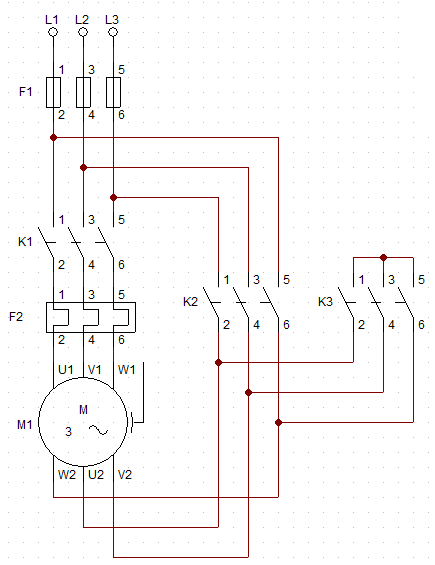
\includegraphics[width=0.4\linewidth]{Figuras/Ch03/fig20.jpg}}
}

\frame{
\frametitle{Sensores térmicos}
\begin{block}{Termopares}
\textbf{Vantagens}:
\begin{itemize}
    \item O diâmetro e o fio não influenciam no potencial gerado.
    \item O tempo de resposta é menor do que qualquer outro medidor de temperatura.
\end{itemize}
\vspace{0.3cm}
\textbf{Desvantagens}:
\begin{itemize}
    \item Eles podem sofrer a corrosão, especialmente quando expostos à temperatura limite superior.
    \item O sinal de saída é dado em milivolt (mV) sendo necessário um aparelho muito sensível para detectá-la.
\end{itemize}
\end{block}
}

\frame{
\frametitle{Sensores térmicos}
\begin{block}{Termistores}
Os sensores \textbf{NTC} e \textbf{PTC} também conhecidos como termistores, são tipos de sensores em que a \textbf{relação entre resistência elétrica e a temperatura} é conhecida. Operam em faixas de temperatura que vão de valores negativos até
aproximadamente $\SI{125}{\degree}$.
\end{block}
\centerline{
\includegraphics[width=0.6\linewidth]{Figuras/Ch03/fig21.jpg}}
}

\frame{
\frametitle{Sensores térmicos}
\centerline{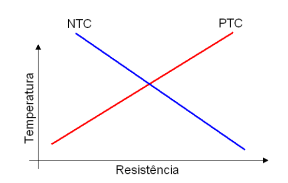
\includegraphics[width=0.7\linewidth]{Figuras/Ch03/fig22.PNG}}
}

\frame{
\frametitle{Sensores térmicos}
\begin{block}{Termistores}
\textbf{Vantagens}:
\begin{itemize}
    \item Grande faixa de aplicações, devido sua versatilidade e baixo custo.
    \item Boa tolerância e precisão.
\end{itemize}
\vspace{0.3cm}
\textbf{Desvantagens}:
\begin{itemize}
    \item Não linearidade.
    \item Inadequação para uso em temperaturas extremas.
\end{itemize}
\end{block}
}

\frame{
\frametitle{Sensores capacitivos}
\begin{block}{}
\textbf{Os sensores de proximidade capacitivos são semelhantes aos sensores de proximidade indutivos} em tamanho, forma e conceito. Entretanto, enquanto os sensores indutivos usam campos magnéticos indutivos para detectar objetos, os sensores de proximidade
capacitivos reagem às alterações do campo
eletrostático, por meio da \textbf{mudança da capacitância da placa detectora} localizada na região denominada face sensível.
\begin{itemize}
    \item Detecção capacitiva é uma tecnologia própria para detectar \textbf{não metais, sólidos e líquidos}. Pode detectar
    \textbf{metais}, porém o custo é mais elevado que o indutivo.
\end{itemize}
\end{block}
\centerline{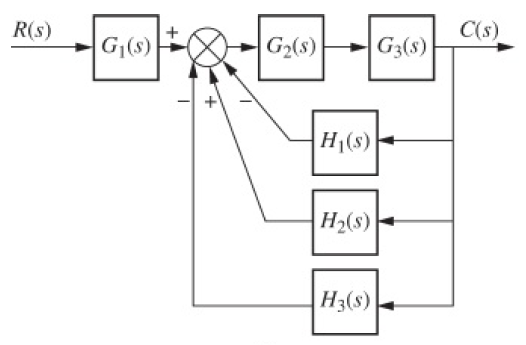
\includegraphics[width=0.7\linewidth]{Figuras/Ch03/fig23.PNG}}
}

\frame{
\frametitle{Sensores capacitivos}
\begin{block}{Aplicação}
Detecção de produto através da embalagem
\end{block}
\centerline{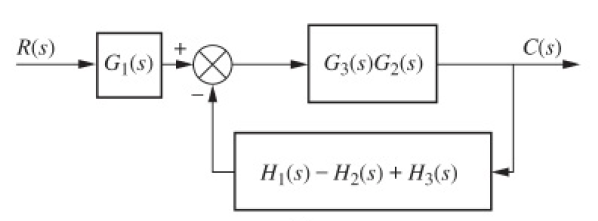
\includegraphics[width=0.7\linewidth]{Figuras/Ch03/fig24.PNG}}
}

\frame{
\frametitle{Sensores capacitivos}
\begin{block}{}
\textbf{Vantagens}:
\begin{itemize}
    \item Detectam metais e não metais, líquidos e sólidos.
    \item  Podem "ver através" de certos materiais (caixas de produto).
    \item Alta vida útil.
\end{itemize}
\vspace{0.3cm}
\textbf{Desvantagens}:
\begin{itemize}
    \item Distância sensora curta.
    \item Muito sensível aos fatores ambientais.
\end{itemize}
\end{block}
}

\frame{
\frametitle{Sensores ultrassônicos}
\begin{block}{}
É um tipo de sensor muito útil na detecção de objetos a uma certa distância, desde que não sejam muito pequenos, para que consigam \textbf{refletir as ondas sonoras}.
\begin{itemize}
    \item Um oscilador \textbf{emite ondas ultrassônicas} (em torno de 42 Khz), que resultam num comprimento de onda da ordem de alguns centímetros, o que permite detectar objetos relativamente pequenos. As ondas refletidas pelo objeto são capitadas pelo sensor, e o \textbf{tempo de resposta é proporcional à distância do objeto}.
\end{itemize}
\end{block}
\centerline{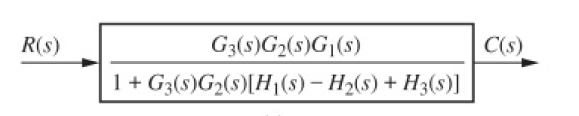
\includegraphics[width=0.7\linewidth]{Figuras/Ch03/fig25.PNG}}
}

\frame{
\frametitle{Sensores ultrassônicos}
\begin{block}{Aplicação}
Medição de nível em tanques
\end{block}
\centerline{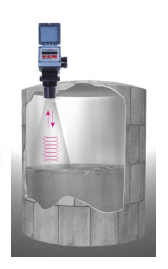
\includegraphics[width=0.3\linewidth]{Figuras/Ch03/fig26.PNG}}
}

\frame{
\frametitle{Sensores ultrassônicos}
\begin{block}{}
\textbf{Vantagens}:
\begin{itemize}
    \item Detectam objetos transparentes, nível de líquido ou superfícies altamente refletivas ou metálicas.
    \item Funcionam bem em ambientes úmidos.
\end{itemize}
\vspace{0.3cm}
\textbf{Desvantagens}:
\begin{itemize}
    \item São suscetíveis a flutuações de temperatura ou vento.
    \item Qualquer ruído acústico na frequência em que o sensor ultrassônico está recebendo pode interferir no desempenho desse sensor. 
\end{itemize}
\end{block}
}

\section*{Referências}
\frame{
\frametitle{Referências e Exercícios Complementares}
\begin{itemize}
\item THOMAZINI, D; ALBUQUERQUE, P. U. B. Sensores Industriais - Fundamentos e Aplicações. 5 ed. São Paulo: Érica, 2005.
\end{itemize}
%\centering{\alert{Página 546 - \textbf{Capítulo 6}}} \\
%\centering{\alert{Lista de exercícios 01}}
}

\frame{
\frametitle{Atuadores}
\begin{block}{Introdução}
\begin{itemize}
    \item São componentes que convertem energia elétrica, hidráulica ou pneumática em \textbf{energia mecânica}.
    \item Através dos sistemas de transmissão, a energia mecânica gerada pelos atuadores é enviada aos links do manipulador para que \textbf{se movimentem}.
    \item Deste modo, podemos definir um atuador como um \textbf{dispositivo destinado a executar uma ação}, como por exemplo, ligação de um motor; movimentação de uma esteira; abertura/fechamento de uma válvula; dosagem de material; etc.
\end{itemize}
\end{block}
}

\frame{
\frametitle{Atuadores}
\begin{block}{Atuadores hidráulicos}
\begin{itemize}
    \item São acionados por \textbf{fluidos em movimento}. Neste caso, o fluido é geralmente \textbf{óleo pressurizado}.
    \item Podem ter a forma de \textbf{cilindros lineares} para gerar os movimentos lineares ou \textbf{cilindros rotativos} para proporcionar deslocamentos angulares.
    \item São conectados a válvulas direcionais, que gerenciam a \textbf{direção do deslocamento} do fluido nos atuadores, a partir de sinais gerados por uma unidade de controle. O custo das válvulas direcionais de alto desempenho ainda é muito elevado.
\end{itemize}
\end{block}
}

\frame{
\frametitle{Atuadores}
\begin{block}{Atuadores hidráulicos}
\begin{itemize}
    \item Permitem a implementação de \textbf{controle contínuo e preciso de posicionamento e velocidade}, devido à incompressibilidade do fluido (óleo hidráulico), resultado numa elevada rigidez. Porém, isso torna \textbf{instável o controle da força}.
    \item Outra característica é a elevada relação entre a potência mecânica transmitida pelo atuador e seu peso, o que possibilita a \textbf{construção de unidades compactas de alta potência}.
    \item Uma bomba fornece o óleo para o atuador através das válvulas direcionais.
\end{itemize}
\end{block}
}

\frame{
\frametitle{Atuadores}
\centerline{
\includegraphics[width=0.9\linewidth]{Figuras/Ch03/fig27.jpg}}
}


\frame{
\frametitle{Atuadores}
\begin{block}{Atuadores pneumáticos}
\begin{itemize}
    \item São acionados por \textbf{fluidos em movimento}. Neste caso, o fluido é geralmente \textbf{ar comprimido}.
    \item Podem ter a forma de \textbf{cilindros lineares} para gerar os movimentos lineares ou \textbf{cilindros rotativos} para proporcionar deslocamentos angulares.
    \item São conectados a válvulas direcionais, que gerenciam a \textbf{direção do deslocamento} do fluido nos atuadores, a partir de sinais gerados por uma unidade de controle. O custo das válvulas direcionais de alto desempenho ainda é muito elevado.
\end{itemize}
\end{block}
}

\frame{
\frametitle{Atuadores}
\begin{block}{Atuadores pneumáticos}
\begin{itemize}
    \item Utilizados em \textbf{robôs industriais} que operam com movimentação de cargas entre posições bem definidas, limitadas por batentes mecânicos.
    \item Devido à \textbf{compressibilidade do fluido} (ar comprimido) possuem \textbf{baixa rigidez}.
    \item Permite que sejam obtidas operações suaves, porém com \textbf{pouca precisão} quanto ao controle de posicionamento entre as posições-limites.
    \item A natureza binária do movimento de cilindros pneumáticos (estendido ou retraído) implica em um \textbf{controle simples e de baixo custo}.
    \item Utiliza um \textbf{compressor} para fornecer o ar comprimido ao atuador pneumático, através das válvulas direcionais.
    \item Para correto funcionamento dos atuadores, recomenda-se a \textbf{instalação de unidades de preparação} (filtro, dreno, regulador de pressão, etc.) no circuito de ar comprimido, antes das válvulas direcionais.
\end{itemize}
\end{block}
}

\frame{
\frametitle{Atuadores}
\centerline{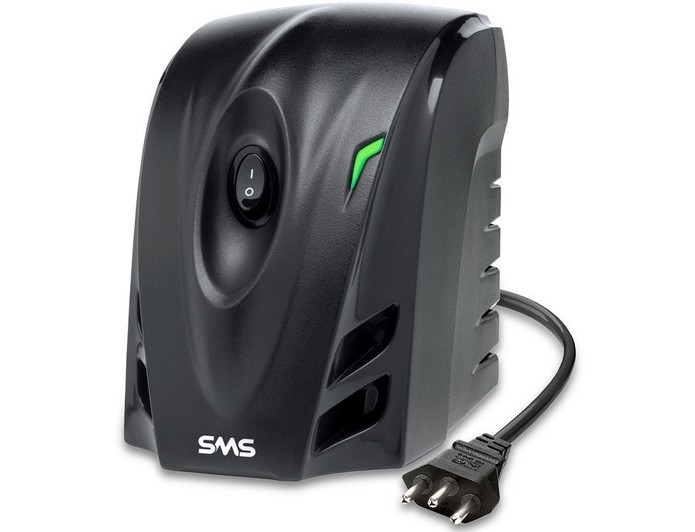
\includegraphics[width=0.9\linewidth]{Figuras/Ch03/fig28.jpg}}
}

\frame{
\frametitle{Atuadores}
\begin{block}{Atuadores eletromagnéticos}
\begin{itemize}
    \item São os atuadores mais utilizados em robôs, principalmente os \textbf{motores C.C.} e os \textbf{motores de passo}.
    \item Possuem as seguintes \textbf{vantagens}: grande variedade de fabricantes e modelos no mercado; motores elétricos, quando associados a sensores, podem ser empregados tanto pra o controle de força quando para o controle de posição do robô; são mais fáceis de programar seus movimentos, já que podem ser controlados por sinais elétricos, permitindo a utilização de controladores de movimento; etc.
\end{itemize}
\end{block}
}

\frame{
\frametitle{Atuadores}
\begin{block}{Atuadores eletromagnéticos - motores de C.C.}
\begin{itemize}
    \item São \textbf{compactos} e geralmente mantém o valor de torque numa faixa constante para grandes variações de velocidade.
    \item \textbf{Necessitam de sensores de posição e de velocidade}, para controle de posicionamento em malha fechada (servocontrole).
    \item A máxima eficiência mecânica desses motores normalmente ocorre a velocidade elevadas, por isso é comum o uso de \textbf{redutores}.
\end{itemize}
\end{block}
}

\frame{
\frametitle{Atuadores}
\centerline{\includegraphics[width=0.9\linewidth]{Figuras/Ch03/fig29.jpg}}
}

\frame{
\frametitle{Atuadores}
\begin{block}{Atuadores eletromagnéticos - motores de passo}
\begin{itemize}
    \item É essencialmente um motor C.C., mas com um \textbf{controle sobre o deslocamento do eixo}. Cada deslocamento angular é chamado de \textbf{passo}.
    \item Podem funcionar em controle de malha aberta, em posição e velocidade, e são facilmente interligados a \textbf{unidades de controle simples e de baixo custo}.
    \item Entretanto, no motores de passo a curva de torque decresce com o aumento de velocidade e, \textbf{em baixas velocidades, podem gerar vibrações mecânicas}.
    \item Em robótica, são mais empregados na \textbf{movimentação de garras}.
    \item O ponto forte de um motor de passo não é a sua força (torque), tampouco sua capacidade de desenvolver altas velocidades - ao contrário da maioria dos outros motores elétricos - mas sim a possibilidade de
    \textbf{controlar seus movimentos de forma precisa}. 
\end{itemize}
\end{block}
}

\frame{
\frametitle{Atuadores}
\centerline{\includegraphics[width=0.5\linewidth]{Figuras/Ch03/fig30.jpg}}
}

\frame{
\frametitle{Atuadores}
\begin{tabular}{ccc}
	\toprule
	\textbf{Hidráulicos} & \textbf{Pneumáticos} & \textbf{Eletromagnéticos} \\ \midrule
	\makecell{Transporte de cargas \\ pesadas} &
	\makecell{Transporte de cargas \\ pequenas e médias} &
	\makecell{Transporte de cargas \\ pequenas e médias} \\ [0.3cm]
	\makecell{Precisão média-alta \\ no controle de posição e \\ velocidade} & Baixa precisão & Alta precisão \\ [0.2cm]
	& \makecell{Altas velocidades e \\ baixo custo}&  Ocupa pouco espaço \\ \bottomrule
\end{tabular}
}

\section*{Referências}
\frame{
\frametitle{Referências e Exercícios Complementares}
\begin{itemize}
\item NATALE, F. Automação Industrial. 10 ed. São Paulo: Érica, 2013.
\end{itemize}
%\centering{\alert{Página 546 - \textbf{Capítulo 6}}} \\
%\centering{\alert{Lista de exercícios 01}}
}
\section{Eletrização por contato e por indução}

\frame{
	\frametitle{Princípio da conservação das cargas}
	\begin{block}{Definição}
		O princípio da conservação da carga elétrica afirma que a soma algébrica das cargas antes e depois de um processo de transferência \textbf{deve ser a mesma}. Assim, podemos dizer que a carga elétrica não pode ser criada nem destruída, somente \textbf{transferida entre corpos}.
	\end{block}
}

\frame{
	\frametitle{Princípio da conservação das cargas}
	\begin{block}{Exemplo}
		Imagine o processo de eletrização por atrito. Inicialmente os corpos a serem friccionados estão neutros, ou seja, apresentam o mesmo número de elétrons e prótons. Após o atrito, um dos corpos cede elétrons e torna-se positivamente eletrizado. O outro  recebe os elétrons, tornando-se negativamente eletrizado. Pela conservação da carga elétrica, podemos dizer que o número de elétrons em excesso em um dos corpos é exatamente igual ao número de prótons em excesso no outro. \textbf{Houve apenas transferência de carga elétrica}.
		\begin{itemize}
			\item A mesma observação pode ser feita a respeito dos processos de eletrização por contato e indução.
		\end{itemize}
	\end{block}
}

\frame{
	\frametitle{Múltiplos e submúltiplos}
	
	\begin{minipage}{0.49\linewidth}
		\resizebox{\textwidth}{!}{
			\begin{tabular}{lcc}
				\toprule
				Prefixo & Símbolo & Expoente \\\midrule
				yocto 	& y & -24\\
				zepto 	& z & -21\\
				atto 	& a &-18\\
				femto 	& f & -15\\
				pico 	& p &-12\\
				nano 	& n &-9\\ 
				micro 	& µ & -6\\
				milli 	& m & -3\\	
				centi 	& c & -2\\	
				deci 	& d &-1\\\bottomrule 
		\end{tabular}}
	\end{minipage}
	\hfill
	\begin{minipage}{0.49\linewidth}
		\resizebox{\textwidth}{!}{
			\begin{tabular}{lcc}
				\toprule
				Prefixo & Símbolo & Expoente \\\midrule
				deca 	& da & 1\\
				hecto 	& h & 2\\
				kilo 	& k & 3\\
				mega 	& M & 6\\
				giga 	& G & 9\\
				tera 	& T & 12\\
				peta 	& P & 15\\
				exa		& E & 18\\
				zetta	& Z & 21\\
				yotta	& Y & 24\\\bottomrule
		\end{tabular}}
	\end{minipage}
	
%	\centerline{\includegraphics[width=1.05\linewidth]{Figuras/Ch04/multiplos.PNG}}
}

\frame{
	\frametitle{Eletrização por contato}
	\begin{block}{Definição}
		Se dois corpos condutores, sendo pelo menos um deles eletrizado, são postos em contato, a carga elétrica tende a se estabilizar, sendo redistribuída entre os dois, fazendo com que \textbf{ambos tenham a mesma carga}, inclusive com \textbf{mesmo sinal}.
	\end{block}
}

\frame{
	\frametitle{Eletrização por contato}
	\centerline{\includegraphics[width=0.7\linewidth]{Figuras/Ch04/conservacao.PNG}}
	\vspace{0.2cm}
	$$\boxed{Q_A + Q_B = Q_{A'} + Q_{B'}}$$
}

\frame{
	\frametitle{Eletrização por contato}
	\begin{block}{O processo - antes}
		\begin{itemize}
			\item O corpo eletrizado transfere cargas elétricas ao corpo neutro, o que ocorre devido à força natural da distribuição de cargas elétricas por dois ou mais materiais condutores.
		\end{itemize}
	\end{block}
	\centerline{\includegraphics[width=0.6\linewidth]{Figuras/Ch04/antes.PNG}}
}

\frame{
	\frametitle{Eletrização por contato}
	\begin{block}{O processo - durante}
		\begin{itemize}
			\item As cargas em excesso do condutor eletrizado negativamente se repelem e alguns elétrons passam para o corpo neutro, fazendo com que ele fique também com elétrons em excesso e, portanto, eletrizado negativamente.
		\end{itemize}
	\end{block}
	\centerline{\includegraphics[width=0.55\linewidth]{Figuras/Ch04/durante.PNG}}
}

\frame{
	\frametitle{Eletrização por contato}
	\begin{block}{O processo - depois}
		\begin{itemize}
			\item Os corpos condutores ficam eletrizados com cargas de mesmo sinal, e não necessariamente em mesma intensidade.
		\end{itemize}
	\end{block}
	\centerline{\includegraphics[width=0.6\linewidth]{Figuras/Ch04/depois.PNG}}
}

\frame{
	\frametitle{Eletrização por contato}
	\begin{block}{Cálculo}
		\begin{itemize}
			\item A troca das cargas depende das dimensões dos condutores.
			\item Se considerarmos que os corpos têm as \textbf{mesmas dimensões e a mesma forma}, sendo, por exemplo, esferas de mesmo raio, \textbf{após o contato apresentarão cargas iguais}.
		\end{itemize}
	
		\vspace{0.2cm}
		$$\boxed{Q' = Q_{A'} = Q_{B'} = \dfrac{Q_A + Q_B}{2}}$$
	\end{block}

}

\frame{
	\frametitle{Eletrização por contato}
	\begin{block}{Exemplo \#01}
		Um corpo condutor A com carga $Q_1 = +\SI{6}{\coulomb} $ é posto em contato com outro corpo neutro $Q_N = \SI{0}{\coulomb} $. Qual é a carga em cada um deles após serem separados?
	\end{block}
}

\frame{
	\frametitle{Eletrização por contato}
	\begin{block}{Resolução}
		\[ Q' = Q_{1'} = Q_{N'} = \dfrac{Q_1 + Q_N}{2} = \dfrac{+6 + 0}{2} = +\SI{3}{\coulomb} \]
	\end{block}
}

\frame{
	\frametitle{Eletrização por contato}
	\begin{block}{Exemplo \#02}
		Um corpo condutor A com carga $Q_A = \SI{-1}{\coulomb} $ é posto em contato com outro corpo condutor B com carga $Q_B = \SI{-3}{\coulomb} $. Após serem separados os dois corpos, o corpo A é posto em contato com um terceiro corpo condutor C de carga $Q_C = +\SI{4}{\coulomb} $. Qual é a carga em cada um após serem separados?
	\end{block}
}

\frame{
	\frametitle{Eletrização por contato}
	\begin{block}{Resolução}
		Para o primeiro contato:
		$$Q' = Q_{A'} = Q_{B'} = \dfrac{Q_A + Q_B}{2} = \dfrac{-1 + (-3)}{2} = \SI{-2}{\coulomb} $$
		
		Para o segundo contato:
		$$Q'' = Q_{A''} = Q_{C''} = \dfrac{Q_A' + Q_C}{2} = \dfrac{-2 + 4}{2} = +\SI{1}{\coulomb} $$
		
		Logo, corpo A possui $+\SI{1}{\coulomb}$, corpo B possui \SI{-2}{\coulomb}, e o corpo C possui $+\SI{1}{\coulomb}$.
	\end{block}
}

\frame{
	\frametitle{Eletrização por contato}
	\begin{block}{E se forem raios diferentes?}
		(UTFPR) Uma esfera metálica A de raio de \SI{20}{\centi\meter} está eletrizada com carga $Q$. Essa esfera é conectada com outra esfera B, depois é desconectada de B e conectada com outra esfera C sendo ainda desconectada de C e conectada com uma esfera D. As esferas B, C e D têm raios de \SI{10}{\centi\meter}, também são metálicas (condutoras) e estavam inicialmente neutras. Verifica-se que a esfera D adquire carga elétrica igual a \SI{4}{\micro\coulomb}. Qual a carga elétrica inicial $Q$, da esfera maior?
	\end{block}
}

\frame{
	\frametitle{Eletrização por contato}
	\begin{block}{Resolução}
		Quando os raios são diferentes o maior fica com mais carga, e a carga é proporcional ao raio -- como o corpo A tem o dobro do raio, ele tem que ficar com o dobro da carga.
		
		\vspace{0.2cm}
		
		Como o corpo A tinha carga $Q$ e o corpo B tinha carga zero no começo, a carga total é $Q$, que deverá permanecer a mesma no final (conservação das cargas).
	\end{block}
}

\frame{
	\frametitle{Eletrização por contato}
	\begin{block}{Resolução}
		Se o corpo B ficar com carga $X$ a carga do A tem que ser $2X$, então $X + 2X = Q$.
		
		\vspace{0.2cm}
		
		Logo, o corpo B fica com carga $Q/3$ e o corpo A com carga $2X = 2Q/3$.
		
		\vspace{0.2cm}
		
		Em seguida o corpo A vai ser colocado em contato com o C. Agora pode-se fazer o mesmo procedimento, começando com o corpo A tendo carga $2Q/3$ e o C carga nula e descobrir a carga final de cada um. Repetir o processo até o final. \alert{Terminar de resolver na lista de exercícios 04!!}
	\end{block}
}

\frame{
	\frametitle{Eletrização por indução eletrostática}
	\begin{block}{Definição}
		Este processo de eletrização é totalmente baseado no \textbf{princípio da atração e repulsão}, já que a eletrização ocorre apenas com a aproximação de um corpo eletrizado (indutor) a um corpo neutro (induzido).
	\end{block}
}

\frame{
	\frametitle{Eletrização por indução eletrostática}
	\begin{block}{Etapas}
		\begin{enumerate}
			\item Primeiramente um bastão eletrizado é aproximado de um condutor inicialmente neutro. Pelo princípio de atração e repulsão, os elétrons livres do induzido são atraídos/repelidos dependendo do sinal da carga do indutor.
		\end{enumerate}
	\end{block}

	\centerline{\includegraphics[width=0.45\linewidth]{Figuras/Ch04/inducao1.PNG}}
}

\frame{
	\frametitle{Eletrização por indução eletrostática}
	\begin{block}{Etapas}
		\begin{enumerate}
			\setcounter{enumi}{1}
			\item O próximo passo é ligar o induzido à terra, ainda na presença do indutor. Os elétrons da terra são conduzidos pelo fio condutor para a parte positiva da esfera no sentido de neutralizá-la.
		\end{enumerate}
	\end{block}

	\centerline{\includegraphics[width=0.45\linewidth]{Figuras/Ch04/inducao2.PNG}}
}

\frame{
	\frametitle{Eletrização por indução eletrostática}
	\begin{block}{Etapas}
		\begin{enumerate}
			\setcounter{enumi}{2}
			\item Desliga-se o induzido da terra. Pode-se retirar o indutor das proximidades e o induzido estará eletrizado com sinal oposto à carga do indutor e as cargas se distribuem por todo o corpo.
		\end{enumerate}
	\end{block}

	\centerline{\includegraphics[width=0.35\linewidth]{Figuras/Ch04/inducao3.PNG}}
}

\frame{
	\frametitle{Eletrização por indução eletrostática}
	\begin{block}{Na natureza}
		Um exemplo de uma consequência da eletrização por indução são os raios. Quando temos uma nuvem carregada eletricamente durante uma tempestade, ela irá induzir na superfície cargas de sinais opostos criando assim um campo elétrico entre a nuvem e a superfície. Se esse campo elétrico for muito intenso teremos uma descarga elétrica violenta que nós conhecemos como raio.
	\end{block}

	\centerline{\includegraphics[width=0.4\linewidth]{Figuras/Ch04/raios.jpg}}
}

\section*{Exercícios}

\frame{
	\frametitle{Exercícios}
	\begin{block}{}
		01. Quatro corpos, A, B, C e D formam um sistema eletricamente isolado. Inicialmente tem-se que $Q_A = \SI{6}{\micro\coulomb} $, $Q_B = \SI{-2}{\micro\coulomb} $, $Q_C = \SI{4}{\micro\coulomb} $ e $Q_D = \SI{-4}{\micro\coulomb} $. O corpo A cede $\SI{2}{\micro\coulomb} $ ao corpo B e o corpo C cede $ \SI{1}{\micro\coulomb} $ ao corpo D. Assinale a afirmação incorreta:\\

		\vspace{0.5cm}

		(a) O corpo B ficou eletricamente neutro. \\

		\vspace{0.3cm}

		(b) A carga total após a transferência é de \SI{4}{\micro\coulomb}. \\

		\vspace{0.3cm}

		(c) A soma algébrica das quantidades de carga elétrica é constante. \\

		\vspace{0.3cm}

		(d) O corpo A, antes e depois, tem carga elétrica positiva. \\

		\vspace{0.3cm}

		(e) Após a transferência de carga os corpos C e D ficaram eletricamente positivos.
	\end{block}
}

\section*{Referências}

\frame{
	\frametitle{Referências e Exercícios Complementares}
	\begin{itemize}
		\item Física, Ciência e Tecnologia – Vol 3. PENTEADO, Paulo César M; TORRES, Carlos Magno A. Ed. Moderna (2006)
	\end{itemize}
	%\centering{\alert{Página 36 - \textbf{1.6.1 até 1.6.5, 1.6.17 até 1.6.19}}} \\
	%https://www.youtube.com/watch?v=IUgS7Uw-qBI
	\centering{\alert{Lista de exercícios 04}}
}
%\section{Introdução ao LibreOffice Impress}

\begin{frame}{}
	\begin{block}{}
		\begin{itemize}
			\item O Impress é o programa de \textbf{apresentações} incluído no LibreOffice.
			\item Você pode criar slides que contenham vários elementos diferentes, incluindo \textbf{texto}, \textbf{listas com marcadores}, \textbf{numeração}, \textbf{tabelas}, \textbf{gráficos} e etc.
			\item O Impress inclui também um \textbf{verificador ortográfico}, um \textbf{dicionário de sinônimos}, \textbf{estilos de texto}, e \textbf{estilos de plano de fundo}.
		\end{itemize}
	\end{block}

	\medskip

	\centering
	\includegraphics[width=0.3\linewidth]{Figuras/Ch05/fig1}
\end{frame}


\begin{frame}{}
	
	\centering
	\includegraphics[width=1\linewidth]{Figuras/Ch05/fig0.1}
\end{frame}


\begin{frame}{Criando um aquivo do Impress}
	\begin{block}{}
		\begin{itemize}
			\item Você pode iniciar o Impress de \textbf{várias formas}, como o Writer.
			\item Quando você iniciar o Impress, a janela principal é exibida.
		\end{itemize}
	\end{block}

	\centering
	\includegraphics[width=0.8\linewidth]{Figuras/Ch05/fig2}
\end{frame}


\begin{frame}{Janela principal do Impress}
	\begin{block}{}
		A janela principal do Impress tem três partes:
		\begin{enumerate}
			\item painel de slides;
			\item área de trabalho;
			\item painel lateral.
		\end{enumerate}
		Além disso, várias \textbf{barras de ferramentas} podem ser \textbf{exibidas} ou \textbf{ocultadas} durante a criação de uma apresentação.
	\end{block}

	\centering
	\includegraphics[width=0.6\linewidth]{Figuras/Ch05/fig3}
\end{frame}


\begin{frame}{Janela principal do Impress}
	\begin{block}{}
		\begin{itemize}
			\item A exibição ou não das partes da Janela Principal do Impress é uma questão de \textbf{preferência} do usuário.
			\item Você pode fechar o Painel de slides ou o Painel lateral, clicando no \textbf{X} no \textbf{canto superior direito} do painel, ou ir em Exibir > Painel de slides ou Exibir > Barra lateral na barra de menu principal para \textbf{desmarcar} o painel.
		\end{itemize}
	\end{block}

	\begin{minipage}{0.49\linewidth}
		\centering
		\includegraphics[width=1\linewidth]{Figuras/Ch05/fig4}
	\end{minipage}\hfill
	\begin{minipage}{0.49\linewidth}
		\centering
		\includegraphics[width=0.75\linewidth]{Figuras/Ch05/fig5}
	\end{minipage}
\end{frame}


\begin{frame}{Janela principal do Impress}
	\begin{block}{}
		\begin{itemize}
			\item Você também pode \textbf{maximizar} a Área de trabalho clicando no \textbf{marcador} Ocultar/Mostrar no meio da linha de separação vertical.
			\item Usar o marcador Ocultar/Mostrar \textbf{esconde}, mas \textbf{não fecha}, os painéis de Slides e Tarefas.
		\end{itemize}
	\end{block}

	\centering
	\includegraphics[width=0.8\linewidth]{Figuras/Ch05/fig6}
\end{frame}


\begin{frame}{Janela principal do Impress}
	\begin{block}{}
		\begin{itemize}
			\item Para \textbf{restaurar} o painel, clique \textbf{novamente} em seu marcador Ocultar/Mostrar.
		\end{itemize}
	\end{block}
	
	\centering
	\includegraphics[width=0.9\linewidth]{Figuras/Ch05/fig7}
\end{frame}


\begin{frame}{Painel de slides}
	\begin{block}{}
		\begin{itemize}
			\item O Painel de slides contém imagens em \textbf{miniatura} dos slides em sua apresentação, na ordem em que serão mostradas.
			\item Clicando em um slide neste painel, este é selecionado e colocado na \textbf{Área de trabalho}.
			\item Quando um slide está na Área de trabalho, você pode \textbf{fazer alterações }nele.
		\end{itemize}
	\end{block}

	\centering
	\includegraphics[width=0.7\linewidth]{Figuras/Ch05/fig8}
\end{frame}


\begin{frame}{Painel de slides}
	\begin{block}{Funções principais}
		Várias \textbf{operações adicionais} podem ser realizadas em \textbf{um ou mais} slides \textbf{simultaneamente} no Painel de slides:
		\begin{itemize}
			\item adicionar \textbf{novos slides} para a apresentação;
			\item marcar um slide como \textbf{oculto} para que ele \textbf{não seja exibido} como parte da apresentação;
			\item \textbf{excluir} um slide da apresentação se ele não for mais necessário;
			\item \textbf{renomear} um slide;
			\item \textbf{duplicar} um slide.
		\end{itemize}
	\end{block}
\end{frame}


\begin{frame}{Painel de slides}
	\begin{block}{Outras funções}
		Também é possível realizar as seguintes operações, embora existam métodos mais eficientes do que usar o Painel de slides:
		\begin{itemize}
			\item \textbf{alterar a transição} de slides seguindo o slide selecionado ou após cada slide em um grupo de slides;
			\item \textbf{alterar o design} de slide;
			\item \textbf{alterar o layout} de slide para um grupo de slides simultaneamente.
		\end{itemize}
	\end{block}
\end{frame}


\begin{frame}{Barra lateral}
	\begin{block}{}
		\begin{itemize}
			\item A Barra lateral tem \textbf{sete seções}.
			\item Para expandir uma seção que você deseja usar, clique no \textbf{ícone}.
			\item Somente \textbf{uma seção} pode ser aberta de cada vez.
		\end{itemize}
	\end{block}

	\centering
	\includegraphics[width=0.19\linewidth]{Figuras/Ch05/fig9}
\end{frame}


\begin{frame}{Barra lateral}
	\begin{block}{Propriedades}
		\begin{itemize}
			\item Mostra os \textbf{leiautes} (\textit{layouts}) incluídos no Impress.
			\item Você pode escolher algum e usá-lo \textbf{como ele é}, ou \textbf{modificá-lo} para atender às suas necessidades.
			\item No entanto, não é possível salvar \textbf{leiautes personalizados}.
		\end{itemize}
	\end{block}

	\centering
	\includegraphics[width=0.4\linewidth]{Figuras/Ch05/fig9.1}
\end{frame}


\begin{frame}{Barra lateral}
	\begin{block}{Transição de slides}
		\begin{itemize}
			\item Fornece acesso a um número de opções de \textbf{transição de slides}.
			\item O padrão é definido como \textbf{Sem transição}, em que o slide seguinte \textbf{substitui} o existente.
			\item No entanto, muitas transições adicionais estão disponíveis.
			\item Você também pode \textbf{especificar} a \textbf{velocidade de transição} (Lenta, Média, Rápida), escolher entre uma transição \textbf{automática} ou \textbf{manual}, e escolher \textbf{quanto tempo} o slide selecionado será mostrado (no caso de transição automática).
		\end{itemize}
	\end{block}
\end{frame}


\begin{frame}{Barra lateral}

	\centering
	\includegraphics[width=0.75\linewidth]{Figuras/Ch05/fig10}
\end{frame}


\begin{frame}{Barra lateral}
	\begin{block}{Animação}
		\begin{itemize}
			\item Uma variedade de \textbf{animações} podem ser usadas para \textbf{realçar} ou \textbf{melhorar} diferentes elementos de cada slide.
			\item A seção Animação fornece uma maneira fácil para \textbf{adicionar}, \textbf{alterar}, ou \textbf{remover animações}.
		\end{itemize}
	\end{block}

	\centering
	\includegraphics[width=0.75\linewidth]{Figuras/Ch05/fig11}
\end{frame}


\begin{frame}{Barra lateral}
	\begin{block}{Slide mestre}
		\begin{itemize}
			\item Aqui você define o \textbf{estilo de página} (slide) para sua apresentação.
			\item O Impress inclui vários \textbf{modelos} de \textbf{páginas mestras} (\textbf{slide mestre}).
			\item Um deles --- Padrão --- é branco, e o restante tem um \textbf{plano de fundo} e \textbf{estilo de texto}.
		\end{itemize}
	\end{block}

	\centering
	\includegraphics[width=0.48\linewidth]{Figuras/Ch05/fig12}
\end{frame}


\begin{frame}{Barra lateral}
	\begin{block}{Estilos}
		\begin{itemize}
			\item Aqui você pode \textbf{editar} e \textbf{aplicar estilos gráficos} e \textbf{criar estilos novos}.
			\item Quando você edita um estilo, as alterações são \textbf{aplicadas automaticamente} a \textbf{todos} os elementos formatados com este estilo em sua apresentação.
		\end{itemize}
	\end{block}

	\centering
	\includegraphics[width=0.43\linewidth]{Figuras/Ch05/fig13}
\end{frame}


\begin{frame}{Barra lateral}
	\begin{block}{Galeria}
		\begin{itemize}
			\item Aqui você pode inserir um \textbf{objeto} em sua apresentação, quer seja como uma \textbf{cópia} ou como um \textbf{link}.
			\item Uma cópia de um objeto é \textbf{independente} do objeto \textbf{original}.
		\end{itemize}
	\end{block}

	\centering
	\includegraphics[width=0.45\linewidth]{Figuras/Ch05/fig14}
\end{frame}


\begin{frame}{Barra lateral}
	\begin{block}{Navegador}
		\begin{itemize}
			\item Aqui você pode trabalhar mais facilmente com objetos e a estrutura da apresentação.
			\item Recomenda-se dar \textbf{nomes significativos} aos \textbf{slides} e \textbf{objetos} em sua apresentação para que você possa \textbf{identificá-los} facilmente quando utilizar a navegação.
		\end{itemize}
	\end{block}

	\centering
	\includegraphics[width=0.4\linewidth]{Figuras/Ch05/fig15}
\end{frame}


\begin{frame}{Alterar formato (tamanho) do slide}
	\begin{block}{Opções de alteração}
		\begin{itemize}
			\item Disponíveis na seção “Propriedades” da Barra lateral, ou;
			\item clicando com o botão direito na área de trabalho e depois, clicar em “Propriedades”.
		\end{itemize}
	\end{block}

	\begin{minipage}{0.49\linewidth}
		\centering
		\includegraphics[width=1\linewidth]{Figuras/Ch05/fig16}
	\end{minipage}\hfill
	\begin{minipage}{0.49\linewidth}
		\centering
		\includegraphics[width=1\linewidth]{Figuras/Ch05/fig16.1}
	\end{minipage}
\end{frame}


\begin{frame}{Alterar formato (tamanho) do slide}
	\begin{block}{Opções de alteração}
		\begin{itemize}
			\item Clicando na barra de menu, clique Slide > Propriedades.
		\end{itemize}
	\end{block}

	\centering
	\includegraphics[width=0.7\linewidth]{Figuras/Ch05/fig16.2}
\end{frame}


\begin{frame}{Alterar formato (tamanho) do slide}
	\begin{block}{Opções de alteração}
		\begin{itemize}
			\item Padrão atual $ \to $ 16:9 Padrão anterior $ \to $ 4:3.
		\end{itemize}
	\end{block}

	\centering
	\includegraphics[width=0.65\linewidth]{Figuras/Ch05/fig16.3}
\end{frame}


\begin{frame}{Preparando uma apresentação}
	\begin{block}{Como fazer uma boa apresentação de slides?}
		\begin{itemize}
			\item Uma boa organização dos slides é crucial para uma apresentação interessante, mas apenas isto não basta.
			\item Dominar o conteúdo é imprescindível para que a apresentação seja bem organizada e bem passada para a plateia.
		\end{itemize}
	\end{block}
\end{frame}



\begin{frame}{Preparando uma apresentação}
	\begin{block}{Como fazer uma boa apresentação de slides?}
		As ideias devem estar encadeadas na \textbf{ordem lógica}:
		\begin{itemize}
			\item capa;
			\item apresentação pessoal (de acordo com a ocasião);
			\item introdução;
			\item desenvolvimento do tema;
			\item conclusão.
		\end{itemize}
	\end{block}

	%	\centering
	%	\includegraphics[width=0.7\linewidth]{Figuras/Ch05/fig}
\end{frame}



\begin{frame}{Preparando uma apresentação}
	\begin{block}{Como fazer uma boa apresentação de slides?}
		\begin{itemize}
			\item Listar apenas \textbf{tópicos}.
			\item Não expressar \textbf{ideias completas} e \textbf{conceitos longos} (apenas se realmente necessários).
			\item \textbf{Evitar acúmulo} de \textbf{caracteres} ou \textbf{ideias diferentes} no mesmo slide.
			\item Imagens devem ser \textbf{explicadas} pelo palestrante.
		\end{itemize}
	\end{block}

	%	\centering
	%	\includegraphics[width=0.7\linewidth]{Figuras/Ch05/fig}
\end{frame}



\begin{frame}{Preparando uma apresentação}
	\begin{block}{Como fazer uma boa apresentação de slides?}
		\begin{itemize}
			\item Usar plano de fundo e fonte \textbf{em contraste}.
			\item O plano de fundo deve \textbf{combinar} com o assunto que trata a apresentação (ou ser neutro).
			\item \textbf{Evitar} o uso de \textbf{cores vibrantes}.
			\item \textbf{evitar} o uso de fonte de \textbf{tamanho pequeno}.
			\item O foco é o \textbf{assunto} e \textbf{não} o que está \textbf{escrito} no slide.
			\item A plateia deve prestar \textbf{mais atenção} no que o \textbf{palestrante tem a dizer} sobre o assunto do que nos slides.
		\end{itemize}
	\end{block}

	%	\centering
	%	\includegraphics[width=0.7\linewidth]{Figuras/Ch05/fig}
\end{frame}



\begin{frame}{Preparando uma apresentação}
	\begin{block}{Como fazer uma boa apresentação de slides?}
		Uma boa apresentação serve \textbf{apenas} para \textbf{direcionar o raciocínio} e deve ser \textbf{ilustrada} com:
		\begin{itemize}
			\item gráficos;
			\item figuras;
			\item fluxogramas;
			\item vídeos;
			\item entre outros \textbf{elementos visuais}...
		\end{itemize}
	\end{block}

	%	\centering
	%	\includegraphics[width=0.7\linewidth]{Figuras/Ch05/fig}
\end{frame}


\begin{frame}{O que não fazer}
	\begin{block}{}
		\begin{itemize}
			\item Vamos observar quais \textbf{problemas} os slides a seguir têm?
		\end{itemize}
	\end{block}

	\centering
	\includegraphics[width=0.7\linewidth]{Figuras/Ch05/fig17}
\end{frame}


\begin{frame}{O que não fazer}
	\centering
	\includegraphics[width=0.7\linewidth]{Figuras/Ch05/fig18}
\end{frame}


\begin{frame}{O que não fazer}
	\centering
	\includegraphics[width=0.7\linewidth]{Figuras/Ch05/fig19}
\end{frame}


\begin{frame}{O que não fazer}
	\centering
	\includegraphics[width=0.7\linewidth]{Figuras/Ch05/fig20}
\end{frame}


\begin{frame}{O que não fazer}
	\centering
	\includegraphics[width=0.7\linewidth]{Figuras/Ch05/fig21}
\end{frame}


\begin{frame}{Tipos de impressão de slides}
	\begin{block}{}
		\begin{itemize}
			\item Antes da impressão de slides, é necessário primeiramente definir a \textbf{utilidade} e o \textbf{tamanho adequado}.
			\item \textbf{Nem sempre} o ideal é imprimir \textbf{um por página}.
			\item Usar a impressão padrão pode \textbf{elevar o custo} e o \textbf{volume de papel}.
			\item Nas opções de impressão, pode-se escolher o \textbf{formato} da impressão:
			\begin{itemize}
				\item Menu Arquivo > Imprimir ou Ctrl + P. (Como no Writer)
			\end{itemize}
		\end{itemize}
	\end{block}

	%	\centering
	%	\includegraphics[width=0.7\linewidth]{Figuras/Ch05/fig}
\end{frame}


\begin{frame}{Tipos de impressão de slides}
%	\begin{block}{}
%		\begin{itemize}
%			\item Para imprimir um por página.
%		\end{itemize}
%	\end{block}

	\centering
	\includegraphics[width=0.75\linewidth]{Figuras/Ch05/fig22}
\end{frame}


\begin{frame}{Tipos de impressão de slides}
	\begin{block}{}
		\begin{itemize}
			\item Para imprimir folhetos.
		\end{itemize}
	\end{block}

	\centering
	\includegraphics[width=0.65\linewidth]{Figuras/Ch05/fig23}
\end{frame}


%\begin{frame}{Atividade 1 --- Usar transições}
%	\begin{block}{}
%		\begin{itemize}
%			\item 
%			Fazer uma apresentação sobre você com as seguintes instruções:
%			Slide 1 → Layout de Título
%			Seu nome completo
%			Slide 2 → Layout de Título e Conteúdo
%			Título – Seu nome completo
%			Tópicos – Gostos e preferências → usar marcadores.
%			Slide 3 → Layout de Título e 2 Conteúdos
%			Título – Seu nome completo
%			Conteúdo 1 – Vida acadêmica (Onde você estudou), usando marcadores;
%			Conteúdo 2 – Inserir tabela – Tabela com informação de curso superior.
%		\end{itemize}
%	\end{block}
%	
%	\centering
%	\includegraphics[width=0.7\linewidth]{Figuras/Ch05/fig}
%\end{frame}


\section*{Exercícios}
\frame{
	\frametitle{Exercícios}
	\begin{block}{}
		01. Você tem vergonha de fazer apresentações? E se tivesse slides para te auxiliar, acha que ficaria mais fácil?
		
		\medskip
		
		02. Você já se imaginou apresentando algo em uma grande companhia ou na faculdade? O que você gostaria de apresentar?
		
		\medskip
		
		03. Monte uma apresentação sobre um assunto que te interessa, ou até sobre o que aprendeu até agora no curso técnico.
	\end{block}
}

\section*{Referências}

\frame{
	\frametitle{Referências e Exercícios Complementares}
	\begin{itemize}
		\item Introdução ao LibreOffice, \href{https://documentation.libreoffice.org/assets/Uploads/Documentation/pt-br/GS50/GS50-IntroducaoLO-5.0-ptbr.pdf}{Apostila de uso livre}.
	\end{itemize}
	%\centering{\alert{Página 36 - \textbf{1.6.1 até 1.6.5, 1.6.17 até 1.6.19}}} \\
	%	\centering{\alert{Lista de exercícios 01}}
}
%\section{Elementos do circuito de comando}

\begin{frame}{Introdução}
\begin{block}{}
\begin{itemize}
    \item Os \textbf{circuitos de comando }são o principal ponto de estudo na disciplina de comandos elétricos, são eles que possibilitam a \textbf{implementação }de uma \textbf{lógica humana }em um dado sistema elétrico.
    \item A \textbf{maior parte }dos elementos elétricos em qualquer sistema é composta de dispositivos de \textbf{comando}.
\end{itemize}
\end{block}
\centerline{\includegraphics[width=0.5\linewidth]{Figuras/Ch06/fig1.jpg}}
\end{frame}

\begin{frame}{Introdução}
\begin{block}{Dispositivos de comando}
\begin{itemize}
    \item Os dispositivos de comando são todos aqueles que possuem função lógica dentro de um circuito elétrico. 
    \item Esses dispositivos realizam sua \textbf{função lógica }\textbf{permitindo }ou \textbf{bloqueando} a passagem de corrente entre dois ou mais pontos do circuito.
\end{itemize}
\end{block}

\begin{minipage}{0.45\linewidth}
	\centering
	\includegraphics[width=0.6\linewidth]{Figuras/Ch06/fig2.jpg}
	
	Lógica NA
\end{minipage}
\hfill
\begin{minipage}{0.45\linewidth}
	\centering
	\includegraphics[width=0.6\linewidth]{Figuras/Ch06/fig3.jpg}
	
	Lógica NF
\end{minipage}
\end{frame}

\begin{frame}{Associação de contatos}
\begin{block}{Associações de contatos NA}
\begin{itemize}
    \item Os dispositivos de comando podem ser \textbf{associados} para realizar funções lógicas mais \textbf{complexas}.
    \item Os contatos NA, por exemplo, podem ser associados das seguintes formas:
\end{itemize}
\end{block}

\begin{minipage}{0.45\linewidth}
	\centering
	\includegraphics[width=0.7\linewidth]{Figuras/Ch06/fig4.jpg}
	
	Associação NA paralelo
\end{minipage}
\hfill
\begin{minipage}{0.45\linewidth}
	\centering
	\includegraphics[width=0.5\linewidth]{Figuras/Ch06/fig5.jpg}
	
	Associação NA série
\end{minipage}
\end{frame}

\begin{frame}{Associação de contatos}
\begin{block}{Associações de contatos NA}
\begin{itemize}
    \item Contatos NA associados em \textbf{paralelo} vão ter o efeito conhecido como "ou", isso é, se um deles \textbf{OU} o outro estiver acionado isso equivale à um \textbf{circuito fechado}.
    \item Na eletrônica digital representamos essa relação com o símbolo "$ + $".
\end{itemize}
\end{block}
\end{frame}

\begin{frame}{Associação de contatos}
\begin{block}{Associações de contatos NA}
	O circuito abaixo pode ser escrito como:
	$$ \text{Carga} = \text{B}1+\text{B}2 $$
	
	isso é, a carga será acionada caso B1 \textbf{OU} B2 sejam acionados (ou os dois ao mesmo tempo, claro).
\end{block}

\centerline{\includegraphics[width=0.35\linewidth]{Figuras/Ch06/fig4.jpg}}
\end{frame}

\newcommand{\nop}{repouso}
\newcommand{\yep}{acionado}

\begin{frame}{Associação de contatos}
\begin{block}{Associações de contatos NA}
	A relação OU também pode ser expressa através de uma \textbf{tabela verdade}, que é útil para entendermos as relações entre os dispositivos de comando e a carga acionada.
	
	Abaixo temos a tabela verdade para a relação:
	$$ \text{Carga} = \text{B}1+\text{B}2 $$
\end{block}

\begin{table}[h]
	\scalebox{1.5}{\begin{tabular}{ccc}
			\toprule
			B1 & B2 & Carga\\ \midrule
			\nop & \nop & \nop \\
			\yep & \nop & \yep \\
			\nop & \yep & \yep \\
			\yep & \yep & \yep \\ \bottomrule
	\end{tabular}}
\end{table}

\end{frame}


\begin{frame}{Associação de contatos}
\begin{block}{Associações de contatos NA}
\begin{itemize}
    \item Contatos NA associados em \textbf{série} vão ter o efeito conhecido como "e", isso é, se um deles \textbf{E} o outro estiverem acionados simultaneamente isso equivale à um \textbf{circuito fechado}.
    \item Na eletrônica digital representamos essa relação com o símbolo "$ \cdot $".
\end{itemize}
\end{block}
\end{frame}

\begin{frame}{Associação de contatos}
\begin{block}{Associações de contatos NA}
	O circuito abaixo pode ser escrito como:
	$$ \text{Carga} = \text{B}1\cdot \text{B}2 $$
	
	 isso é, a carga será acionada caso B1 \textbf{E} B2 sejam acionados simultaneamente.
\end{block}

\centerline{\includegraphics[height=0.5\textheight]{Figuras/Ch06/fig5.jpg}}
\end{frame}

\begin{frame}{Associação de contatos}
\begin{block}{Associações de contatos NA}
	Abaixo temos a tabela verdade para a relação:
	$$ \text{Carga} = \text{B}1\cdot \text{B}2 $$
\end{block}

\vspace{0.3cm}

\begin{table}[h]
	\scalebox{1.5}{\begin{tabular}{ccc}
			\toprule
			B1 & B2 & Carga\\ \midrule
			\nop & \nop & \nop \\
			\yep & \nop & \nop \\
			\nop & \yep & \nop \\
			\yep & \yep & \yep \\ \bottomrule
	\end{tabular}}
\end{table}
\end{frame}


\begin{frame}{Associação de contatos}
\begin{block}{Associações de contatos NF}
\begin{itemize}
    \item Os contatos NF podem ser associados das mesma formas que os contatos NA:
\end{itemize}
\end{block}

\begin{minipage}{0.45\linewidth}
	\centering
	\includegraphics[width=0.7\linewidth]{Figuras/Ch06/fig6.jpg}
	
	Associação NF paralelo
\end{minipage}
\hfill
\begin{minipage}{0.45\linewidth}
	\centering
	\includegraphics[width=0.5\linewidth]{Figuras/Ch06/fig7.jpg}
	
	Associação NF série
\end{minipage}
\end{frame}


\begin{frame}{Associação de contatos}
\begin{block}{Associações de contatos NF}
\begin{itemize}
    \item As associações de contatos são universais e possuem a mesma simbologia independendo de os contatos serem NA ou NF. Os contatos NF, porém, serão simbolizados de forma diferente, ganhando uma barra em cima do símbolo.
    \item O contato abaixo, por exemplo, pode ser simbolizado por "$ \overline{\text{B}1} $".
\end{itemize}
\end{block}

\vspace{0.2cm}

\begin{center}
	\begin{tikzpicture}[scale=1.5]
	\draw (1.8,0.3) -- +(0.2,0) (1.8,0.3) -- ++(0,0.4) -- +(0.2,0);
	\draw[loosely dashed] (1.8,0.5) -- +(0.85,0);
	\draw (2,0) ++(0.5, 1) -- +(0,0.2) (2,0) ++(0.5,0) -- +(0,-0.2);
	\draw (2,0) ++(0.5,0) -- ++(0.3,1) -- +(-0.3,0);
	\node at (1.5, 0.5) {B1};
	\end{tikzpicture}
\end{center}
\end{frame}

\begin{frame}{Associação de contatos}
\begin{block}{Associações de contatos NF}
O circuito abaixo pode ser escrito como: 
$$ \text{Carga} = \overline{\text{B}1}+\overline{\text{B}2} $$ 

isso é, a carga será acionada caso B1 \textbf{OU} B2 estejam em repouso (ou os dois ao mesmo tempo, claro).
\end{block}

\centerline{\includegraphics[height=0.5\textheight]{Figuras/Ch06/fig6.jpg}}
\end{frame}

\begin{frame}{Associação de contatos}
\begin{block}{Associações de contatos NF}
Abaixo temos a tabela verdade para a relação:
$$ \text{Carga} = \overline{\text{B}1}+\overline{\text{B}2} $$
\end{block}

\vspace{0.3cm}

\begin{table}[h]
\scalebox{1.5}{\begin{tabular}{ccc}
	\toprule
	B1 & B2 & Carga\\ \midrule
	\nop & \nop & \yep \\
	\yep & \nop & \yep \\
	\nop & \yep & \yep \\
	\yep & \yep & \nop \\ \bottomrule
\end{tabular}}
\end{table}

\end{frame}


\begin{frame}{Associação de contatos}
\begin{block}{Associações de contatos NF}
O circuito abaixo pode ser escrito como:
$$ \text{Carga} = \overline{\text{B}1}\cdot\overline{\text{B}2} $$

isso é, a carga será acionada caso B1 \textbf{E} B2 estejam em repouso simultaneamente.
\end{block}

\centerline{\includegraphics[height=0.5\textheight]{Figuras/Ch06/fig7.jpg}}
\end{frame}

\begin{frame}{Associação de contatos}
\begin{block}{Associações de contatos NF}
Abaixo temos a tabela verdade para a relação:
$$ \text{Carga} = \overline{\text{B}1}\cdot\overline{\text{B}2} $$
\end{block}

\vspace{0.3cm}

\begin{table}[h]
\scalebox{1.5}{\begin{tabular}{ccc}
\toprule
B1 & B2 & Carga\\ \midrule
\nop & \nop & \yep \\
\yep & \nop & \nop \\
\nop & \yep & \nop \\
\yep & \yep & \nop \\ \bottomrule
\end{tabular}}
\end{table}
\end{frame}


\begin{frame}{Elementos do circuito de comando}
\begin{block}{Principais elementos}
	Os principais elementos estudados em comandos elétricos são:
	\begin{itemize}
		\item Botões (botoeiras)
		\item Contatores
		\item Relés
		\item Temporizadores
	\end{itemize}
	Todos eles possuem função lógica, podendo ser eles próprios ou suas chaves associados como vimos anteriormente.
\end{block}
\end{frame}


\begin{frame}{Elementos do circuito de comando}
\begin{block}{Botões (botoeiras)}
	Os botões já foram discutidos anteriormente, mas vale citar:
	\begin{itemize}
		\item A botoeira é um \textit{elemento de sinal}, isto é, deve ser usada somente no circuito de comando para enviar sinais à outros componentes.
		\item Na indústria usamos o nome "botoeira", pois esta possui retorno por mola. Isso é essencial para o funcionamento lógico adequado deste elemento. 
	\end{itemize}
\end{block}
\end{frame}


\begin{frame}{Elementos do circuito de comando}
\begin{block}{Contatores}
	Os contatores também já foram abordados anteriormente, mas vale a pena mencionar seu princípio de funcionamento:
	\begin{itemize}
		\item A parte em cinza consiste em um núcleo magnético fragmentado em duas partes, um delas sendo móvel.
	\end{itemize}
\end{block}

\centerline{\includegraphics[width=0.3\linewidth]{Figuras/Ch06/fig8.jpg}}
\end{frame}

\begin{frame}{Elementos do circuito de comando}
\begin{block}{Contatores}
	\begin{itemize}
		\item Quando as bobinas (em laranja) são percorridas por corrente geram um fluxo magnético que junta as duas partes magnéticas, movimentando consigo os contatos do componente, que podem se abrir (NF) ou fechar (NA).
	\end{itemize}
\end{block}

\begin{minipage}{0.45\linewidth}
	\centering
	\includegraphics[width=0.6\linewidth]{Figuras/Ch06/fig8.jpg}
	
	Contator desenergizado
\end{minipage}\tikzmark{C1}
\hfill
\begin{minipage}{0.45\linewidth}
	\centering
	\includegraphics[width=0.6\linewidth]{Figuras/Ch06/fig9.jpg}
	
	Contator energizado
\end{minipage}

\begin{tikzpicture}[overlay, remember picture]
	\draw[-{Latex[length=4mm,width=5mm]}, line width=1.5mm] (C1) -- +(1,0);
\end{tikzpicture}

\end{frame}

\begin{frame}{Elementos do circuito de comando}
\begin{block}{Contatores}
	\begin{itemize}
		\item Quando o fluxo de corrente cessa os núcleos magnéticos são separados por molas.
	\end{itemize}
\end{block}
\begin{minipage}{0.45\linewidth}
	\centering
	\includegraphics[width=0.6\linewidth]{Figuras/Ch06/fig9.jpg}
	
	Contator energizado
\end{minipage}\tikzmark{C1}
\hfill
\begin{minipage}{0.45\linewidth}
	\centering
	\includegraphics[width=0.6\linewidth]{Figuras/Ch06/fig8.jpg}
	
	Contator desenergizado
\end{minipage}

\begin{tikzpicture}[overlay, remember picture]
\draw[-{Latex[length=4mm,width=5mm]}, line width=1.5mm] (C1) -- +(1,0);
\end{tikzpicture}

\end{frame}

\begin{frame}{Elementos do circuito de comando}
	\centerline{\includegraphics[width=1\linewidth]{Figuras/Ch06/fig10.jpg}}
\end{frame}


\begin{frame}{Elementos do circuito de comando}
\begin{block}{Relés}
\begin{itemize}
    \item Os relés são elementos muito similares aos contatores, porém possuem \textbf{capacidade reduzida}.
    \item Na imagem abaixo podemos notar que os componentes estruturais presentes no relé são muito similares aos do contator. Não há, porém, um núcleo magnético móvel, as únicas coisas que se movem são os \textbf{contatos}.
\end{itemize}
\end{block}
\centerline{\includegraphics[width=0.45\linewidth]{Figuras/Ch06/fig11.png}}
\end{frame}


\begin{frame}{Elementos do circuito de comando}
\begin{block}{Relés}
\begin{itemize}
    \item Uma aplicação mais interessante dos relés é a proteção do equipamento de potência no circuito de força. Essa proteção é feita pelos chamados \textit{relés térmicos}, que também já foram abordados.
\end{itemize}
\end{block}
\centerline{\includegraphics[width=0.5\linewidth]{Figuras/Ch06/fig12.jpg}}
\end{frame}


\begin{frame}{Elementos do circuito de comando}
\begin{block}{Relés}
\begin{itemize}
    \item Outra possível aplicação dos relés é a \textbf{temporização}. Relés com essa função são chamados de relés \textit{de tempo} ou \textit{temporizadores}.
    \item A simbologia dos relés temporizadores e seus contatos é apresentada abaixo.
\end{itemize}
\end{block}
\smallskip
\centerline{\includegraphics[width=0.8\linewidth]{Figuras/Ch06/fig13.jpg}}
\end{frame}


\begin{frame}{Elementos do circuito de comando}
\begin{block}{Relés}
	\begin{itemize}
		\item Repare que os contatos do relé temporizador são representados por uma chave com \textbf{duas} posições.
		\item Quando o relé está em repouso, os terminais 55-56 estão ligados e quando o relé está acionado os terminais 55-58 se ligam.
	\end{itemize}
\end{block}
\centerline{\includegraphics[width=0.6\linewidth]{Figuras/Ch06/fig14.jpg}}
\end{frame}


\begin{frame}{Elementos do circuito de comando}
\begin{minipage}{0.45\linewidth}
	\centering
	\includegraphics[width=1.3\linewidth]{Figuras/Ch06/fig15.jpg}
\end{minipage}
\hfill
\begin{minipage}{0.45\linewidth}
	\centering
	\includegraphics[width=0.6\linewidth]{Figuras/Ch06/fig16.jpg}
\end{minipage}
\end{frame}


\begin{frame}{Elementos do circuito de comando}
\begin{block}{Simbologia}
	\begin{itemize}
		\item Segue abaixo uma tabela apresentando os símbolos literais de acordo com a NBR 5280.
	\end{itemize}
	 \textbf{Nota:} É comum a utilização de "B"~para designar botão.
\end{block}
\begin{table}[h]
	\scalebox{1}{\begin{tabular}{cl}
			\toprule
			Símbolo & \multicolumn{1}{c}{Componente}\\\midrule
			F & Dispositivos de proteção \\
			H & Dispositivos de sinalização \\
			K & Contatores \\
			M & Motores\\
			\multirow{2}{*}{Q} & Dispositivos de manobra \\
			 & para circuitos de potência \\
			\multirow{2}{*}{S} & Dispositivos de manobra e \\
			 & seletores auxiliares \\
			T & Transformadores \\
			\bottomrule
	\end{tabular}}
\end{table}
\end{frame}


\begin{frame}{Elementos do circuito de comando}
\begin{block}{Simbologia}
	A numeração dos contatos que representam terminais de força é feita da seguinte maneira:
	\begin{itemize}
		\item Entrada (linha): 1, 3 e 5
		\item Saída (terminal): 2, 4 e 6
	\end{itemize}
	Já a numeração dos contatos auxiliares segue o seguinte padrão:
	\begin{itemize}
		\item Contato NF: 1 (entrada) e 2 (saída)
		\item Contato NA: 3 (entrada) e 4 (saída)
	\end{itemize}
	Os terminais da bobina de relés e contatores são designados por A1 e A2. Os contatos auxiliares de um contator seguem uma numeração com dois dígito, sendo:
	\begin{itemize}
		\item 1o dígito: indica o número do contato (1, 2, 3...)
		\item 2o dígito: indica o tipo do contato (NA ou NF)
	\end{itemize}
\end{block}
\end{frame}


\frame{
	\frametitle{Exercícios}
	\begin{block}{}
		01. Dar exemplos da utilização de relés temporizadores.
		
		\vspace{0.5cm}
		
		02. Desenhar e fazer a tabela verdade do circuito expresso por: \[ \text{Carga}=\overline{\text{B}1}+\text{B}2 \]
	\end{block}
}

\section*{Referências}
\frame{
	\frametitle{Referências e Exercícios Complementares}
	\begin{itemize}
		\item FILHO, João Mamede. Instalações Elétricas Industriais, 6 ed. Rio de Janeiro, LTC, 2001.
	\end{itemize}
	%\centering{\alert{Página 546 - \textbf{Capítulo 6}}} \\
	%\centering{\alert{Lista de exercícios 01}}
}

%\section{Arranjos básicos e exemplos de circuitos}

\begin{frame}{Introdução aos arranjos}
\begin{block}{}
	Quando discutimos o exemplo do portão do sítio o acionamento do motor foi resolvido com um botão e um contator.
	\begin{itemize}
		\item Como fazemos para manter o portão aberto?
		\item Como fazemos para fechá-lo?
	\end{itemize}
	Os arranjos podem resolver esses problemas.
\end{block}

\centerline{\includegraphics[width=0.6\linewidth]{Figuras/Ch07/fig0.jpg}}
\end{frame}

\begin{frame}{Exemplo \#01}
\begin{block}{Contextualização}
	Quando damos a partida em um carro, ele se mantém ligado até darmos outro comando (ou se deixarmos o motor "morrer").
	
	\begin{itemize}
		\item Como fazer o motor se "lembrar"~da última ordem dada?
	\end{itemize}
\end{block}

\centerline{\includegraphics[width=0.8\linewidth]{Figuras/Ch07/fig1.jpg}}
\end{frame}


\begin{frame}{Exemplo \#01}
\begin{block}{Selo}
\begin{itemize}
    \item Podemos colocar uma chave auxiliar do contator do motor em paralelo com nosso botão de acionamento.
    \item Existe um problema com o circuito abaixo. Você consegue encontrá-lo?
\end{itemize}
\end{block}

\centerline{\includegraphics[height=0.65\textheight]{Figuras/Ch07/fig2.jpg}}
\end{frame}


\begin{frame}{Exemplo \#01}
\begin{block}{Selo}
\begin{itemize}
    \item O circuito de selo (ou de \textit{memória}) possui dois botões diferentes, um para ligá-lo e outro para desligá-lo.
\end{itemize}
\end{block}

\centerline{\includegraphics[height=0.7\textheight]{Figuras/Ch07/fig3.jpg}}
\end{frame}


\begin{frame}{Exemplo \#01}
\begin{block}{Selo}
\begin{itemize}
    \item Para \textbf{garantir} a memória em um circuito é possível colocar mais de um contator em paralelo com nossa chave de acionamento.
\end{itemize}
 \textbf{Nota:} A bobina de K2 não está representada.
\end{block}

\centerline{\includegraphics[height=0.55\textheight]{Figuras/Ch07/fig4.jpg}}
\end{frame}


\begin{frame}{Exemplo \#02}
\begin{block}{Contextualização}
\begin{itemize}
    \item Voltando ao nosso carro, precisamos dar ré para sair da garagem de casa.
    \item Como isso funciona?
\end{itemize}
\end{block}

\centerline{\includegraphics[width=0.65\linewidth]{Figuras/Ch07/fig5.jpg}}
\end{frame}


\begin{frame}{Exemplo \#02}
\begin{block}{Direção de rotação}
\begin{itemize}
    \item Em motores industriais podemos inverter a rotação de um motor invertendo duas de suas fases na entrada.
\end{itemize}
\end{block}
\begin{minipage}{0.45\linewidth}
	\centering
	\includegraphics[width=0.6\linewidth]{Figuras/Ch07/fig6.jpg}
\end{minipage}
\hfill
\begin{minipage}{0.45\linewidth}
	\centering
	\includegraphics[width=0.65\linewidth]{Figuras/Ch07/fig7.jpg}
\end{minipage}
\end{frame}


\begin{frame}{Exemplo \#02}
\begin{block}{Direção de rotação}
\begin{itemize}
    \item Se quisermos fazer nosso motor mudar de rotação com o apertar de um botão (ou engatando uma marcha específica) podemos fazer um circuito com dois contatores, cada um em uma configuração de rotação específica.
\end{itemize}
\end{block}
\centerline{\includegraphics[height=0.6\textheight]{Figuras/Ch07/fig8.jpg}}
\end{frame}


\begin{frame}{Exemplo \#02}
\begin{block}{Intertravamento}
\begin{itemize}
    \item Se ligarmos esses dois contatores ao mesmo tempo fecharemos um curto em nosso motor.
    \item Para resolver esse problema usamos o \textbf{intertravamento}.
\end{itemize}
\end{block}
\centerline{\includegraphics[height=0.6\textheight]{Figuras/Ch07/fig9.jpg}}
\end{frame}

\begin{frame}{Exemplo \#02}
\begin{block}{Intertravamento}
\begin{itemize}
    \item Quando apertamos o botão B1, o contator K1 se aciona e abre a passagem que liga o contator K2. O mesmo acontece se apertarmos B2 e K1 estiver em repouso.
    \item Um contator "trava"~o funcionamento do outro.
    \item É \textbf{essencial} que a chave auxiliar que realiza a trava esteja em \textbf{série} com o circuito de acionamento do contator que deve travar, caso contrário a trava não funciona.
\end{itemize}
\end{block}
\end{frame}


\begin{frame}{Exemplo \#02}
\begin{block}{Intertravamento}
\begin{itemize}
    \item Se quisermos aumentar o nível de segurança podemos compor a trava com mais chaves auxiliares.
\end{itemize}
\end{block}
\centerline{\includegraphics[width=0.2\linewidth]{Figuras/Ch07/fig10.jpg}}
\end{frame}


\begin{frame}{Exemplo \#02}
\begin{block}{Ligamento condicional}
\begin{itemize}
    \item Uma configuração com o efeito oposto ao do intertravamento é o \textit{ligamento condicional}.
\end{itemize}
\end{block}
\centerline{\includegraphics[width=0.2\linewidth]{Figuras/Ch07/fig11.jpg}}
\end{frame}


\begin{frame}{Exemplos de circuitos elétricos}
\begin{block}{}
	Agora, vamos ilustrar alguns circuitos utilizados comumente para acionar motores.
	
	Os elementos básicos nos comandos elétricos são:
	
	\begin{itemize}
		\item Dispositivos de manobra
		\item Dispositivos de proteção (curto e sobrecarga)
		\item Seccionamento
		\item Equipamento de potência
	\end{itemize}

	Você consegue identificar esses elementos nos exemplos?
\end{block}
\end{frame}


\begin{frame}{Partida direta}
\centerline{\includegraphics[width=0.7\linewidth]{Figuras/Ch07/fig12.jpg}}
\end{frame}

\begin{frame}{Partida direta com sinalização}
\centerline{\includegraphics[width=1\linewidth]{Figuras/Ch07/fig13.jpg}}
\end{frame}

\begin{frame}{Partida direta com reversão}
\centerline{\includegraphics[height=0.9\textheight]{Figuras/Ch07/fig14.jpg}}
\end{frame}


\begin{frame}{Exemplos de circuitos elétricos}
\begin{block}{Tipos de partidas}
\begin{itemize}
    \item Motores industriais são equipamentos caros e que precisam de cuidados especiais.
    \item Existem diferentes formas acionar um motor, cada qual com seus benefícios e fraquezas.
    \item Vamos explorar três formas de acionar um motor usando ligações estrela e triângulo.
\end{itemize}
\end{block}
\end{frame}


\begin{frame}{Exemplos de circuitos elétricos}
\begin{block}{Princípio das ligações de motores}
\begin{itemize}
    \item Um motor trifásico é composto por três bobinas que podem ser ligadas entre si de diferentes maneiras.
\end{itemize}
\end{block}
\centerline{\includegraphics[width=0.6\linewidth]{Figuras/Ch07/fig15.jpg}}
\end{frame}


\begin{frame}{Exemplos de circuitos elétricos}
\begin{block}{Princípio das ligações de motores}
\begin{itemize}
    \item Em eletrônica podemos conectar três bobinas das seguintes maneiras:
\end{itemize}
\end{block}

\vspace{1.5cm}
\begin{minipage}{0.45\linewidth}
	\centering
	\begin{circuitikz}[x=1.5cm, y=1.5cm]
		\draw (0,1) to[short, o-*] ++(1,0) to[L] ++(0,-1) to[short, *-o] ++(-1,0);
		\draw (1,1) to[short, -*] ++(1,0) to[L] ++(0,-1) to[short, *-] ++(-1,0);
		\draw (2,1) to[short] ++(1,0) to[L] ++(0,-1) to[short] ++(-1,0);
	\end{circuitikz}
	
	Em paralelo
\end{minipage}
\hfill
\begin{minipage}{0.45\linewidth}
	\centering
	\begin{circuitikz}[x=1.5cm, y=1.5cm]
		\draw (0,1) to[short, o-] ++(0.2,0) to[L] ++(1,0) to[L] ++(1,0) to[L] ++(1,0) to[short, -o] ++(0.2,0);
	\end{circuitikz}
	
	Em série
\end{minipage}
\end{frame}


\begin{frame}{Exemplos de circuitos elétricos}
\begin{block}{Princípio das ligações de motores}
	Mas, como estamos lidando com um sistema trifásico, precisamos adaptar um pouco.
\end{block}

\vspace{0.5cm}
\begin{minipage}{0.45\linewidth}
	\centering
	\includegraphics[width=\linewidth]{Figuras/Ch07/fig16.jpg}
	
	Em paralelo, o que vamos chamar de \textbf{estrela} (Y)
\end{minipage}
\hfill
\begin{minipage}{0.45\linewidth}
	\centering
	\includegraphics[width=\linewidth]{Figuras/Ch07/fig17.jpg}
	
	Em série, o que vamos chamar de \textbf{triângulo} ($ \Delta $)
\end{minipage}

\end{frame}

\begin{frame}{Exemplos de circuitos elétricos}
\begin{block}{Ligação Y}
\begin{itemize}
    \item Na ligação estrela nosso motor tem menos força, e por isso, se estiver parado, sentirá menos impacto quando for acionado.
    \item É ideal para \textbf{ligar} o motor, mas \textbf{não} para \textbf{trabalhar} com ele.
\end{itemize}
\end{block}
\end{frame}


\begin{frame}{Exemplos de circuitos elétricos}
\centerline{\includegraphics[height=0.9\textheight]{Figuras/Ch07/fig18.jpg}}
\end{frame}


\begin{frame}{Exemplos de circuitos elétricos}
\begin{block}{Ligação $ \Delta $}
\begin{itemize}
    \item Na ligação triângulo nosso motor tem mais força, por isso é usada na hora de trabalhar com grandes cargas.
    \item É ideal para \textbf{trabalhar} com motor, mas \textbf{não} para \textbf{acioná-lo}.
\end{itemize}
\end{block}
\end{frame}


\begin{frame}{Exemplos de circuitos elétricos}
\centerline{\includegraphics[height=0.9\textheight]{Figuras/Ch07/fig19.jpg}}
\end{frame}


\begin{frame}{Exemplos de circuitos elétricos}
\begin{block}{Partida Y-$ \Delta $}
\begin{itemize}
    \item Podemos unir o útil ao agradável através do uso de \textbf{temporizadores}, dando a partida no nosso motor usando a ligação estrela e, depois, trabalhar com ele na ligação triângulo.
\end{itemize}
\end{block}
\end{frame}


\begin{frame}{Exemplos de circuitos elétricos}
\centerline{\includegraphics[height=0.9\textheight]{Figuras/Ch07/fig20.jpg}}
\end{frame}


\begin{frame}{Exemplos de circuitos elétricos}
\centerline{\includegraphics[height=0.9\textheight]{Figuras/Ch07/fig21.jpg}}
\end{frame}


\begin{frame}{Exemplos de circuitos elétricos}
\centerline{\includegraphics[height=0.9\textheight]{Figuras/Ch07/fig22.jpg}}
\end{frame}


\frame{
	\frametitle{Exercícios}
	\begin{block}{}
		01. Dar um exemplo de uso de dois arranjos em conjunto.
		
		\vspace{0.5cm}
		
		02. Esboçar o circuito do exemplo dado na questão 01.
	\end{block}
}

\section*{Referências}
\frame{
	\frametitle{Referências e Exercícios Complementares}
	\begin{itemize}
		\item FILHO, João Mamede. Instalações Elétricas Industriais, 6 ed. Rio de Janeiro, LTC, 2001.
	\end{itemize}
	%\centering{\alert{Página 546 - \textbf{Capítulo 6}}} \\
	%\centering{\alert{Lista de exercícios 01}}
}
%\section*{Circuitos combinacionais II}

\frame{
	\frametitle{Códigos binários - BCD 8421}
	\begin{block}{BCD 8241}
		\begin{itemize}
			\item BCD: \textit{binary coded decimal}.
			\item Técnica mais simples e normal de ser utilizada -- \textbf{natural}.
			\item Cada dígito binário é representado pelo seu correspondente binário de 4 dígitos.
			\item 8421 indica os "pesos" de cada algarismo no sistema binário.
			\item A grande vantagem do sistema BCD 8421 é a facilidade  entre homem-máquina.
			\item O código BCD, no entanto, é menos eficiente que o código binário puro, pois são usados \textbf{mais bits }para se representar um determinado valor.
		\end{itemize}
	\end{block}
}

\frame{
	\frametitle{Códigos binários - BCD 8421}
	
	\renewcommand{\arraystretch}{1}
	\centering
	\begin{adjustbox}{totalheight=0.75\textheight-2\baselineskip}
	\centering
	\begin{tabular}{c|cccc}
		\toprule
		\multirow{2}{*}{\makecell{\normalsize Decimal}} & \multicolumn{4}{c}{\makecell{\normalsize BCD 8421}} \\ \cmidrule{2-5}
		  & A & B & C & D \\ \midrule
		0 & 0 & 0 & 0 & 0 \\
		1 & 0 & 0 & 0 & 1 \\
		2 & 0 & 0 & 1 & 0 \\
		3 & 0 & 0 & 1 & 1 \\
		4 & 0 & 1 & 0 & 0 \\
		5 & 0 & 1 & 0 & 1 \\
		6 & 0 & 1 & 1 & 0 \\
		7 & 0 & 1 & 1 & 1 \\
		8 & 1 & 0 & 0 & 0 \\
		9 & 1 & 0 & 0 & 1 \\ \bottomrule
	\end{tabular}
	\end{adjustbox}

	\begin{block}{}
		\begin{itemize}
			\setlength\itemsep{0.25em}
			\item $ \mathsmaller{10 = 0001\; \! 0000} $
			\item $ \mathsmaller{11 = 0001\; \! 0001} $
			\item $ \mathsmaller{\ldots} $
			\item $ \mathsmaller{15 = 0001\; \! 0101} $
		\end{itemize}
	\end{block}
}

\frame{
	\frametitle{Códigos binários - BCD 7421}
	
%	\renewcommand{\arraystretch}{1}
	\centering
	\begin{adjustbox}{totalheight=1\textheight-2\baselineskip}
		\centering
		\begin{tabular}{c|cccc}
			\toprule
			\multirow{2}{*}{\makecell{\normalsize Decimal}} & \multicolumn{4}{c}{\makecell{\normalsize BCD 7421}} \\ \cmidrule{2-5}
			& A & B & C & D \\ \midrule
			0 & 0 & 0 & 0 & 0 \\
			1 & 0 & 0 & 0 & 1 \\
			2 & 0 & 0 & 1 & 0 \\
			3 & 0 & 0 & 1 & 1 \\
			4 & 0 & 1 & 0 & 0 \\
			5 & 0 & 1 & 0 & 1 \\
			6 & 0 & 1 & 1 & 0 \\
			7 & 1 & 0 & 0 & 0 \\
			8 & 1 & 0 & 0 & 1 \\
			9 & 1 & 0 & 1 & 0 \\ \bottomrule
		\end{tabular}
	\end{adjustbox}
}

\frame{
	\frametitle{Códigos binários - Excesso 3}
	
	\begin{block}{}
		\begin{itemize}
			\item Transformação do número decimal no binário correspondente somando-se 3 unidades.
			\item É obtido adiantando o código BCD três vezes.
			\item Neste modelo há apenas de zero a nove decimal.
			\item Apresenta algumas vantagens nas operações matemáticas - utilizado em circuitos aritméticos.
		\end{itemize}
	\end{block}
}

\frame{
	\frametitle{Códigos binários - Excesso 3}
	
%	\renewcommand{\arraystretch}{1}
	\centering
	\begin{adjustbox}{totalheight=1\textheight-2\baselineskip}
		\centering
		\begin{tabular}{c|cccc}
			\toprule
			\multirow{2}{*}{\makecell{\normalsize Decimal}} & \multicolumn{4}{c}{\makecell{\normalsize Excesso 3}} \\ \cmidrule{2-5}
			& A & B & C & D \\ \midrule
			0 & 0 & 0 & 1 & 1 \\
			1 & 0 & 1 & 0 & 0 \\
			2 & 0 & 1 & 0 & 1 \\
			3 & 0 & 1 & 1 & 0 \\
			4 & 0 & 1 & 1 & 1 \\
			5 & 1 & 0 & 0 & 0 \\
			6 & 1 & 0 & 0 & 1 \\
			7 & 1 & 0 & 1 & 0 \\
			8 & 1 & 0 & 1 & 1 \\
			9 & 1 & 1 & 0 & 0 \\ \bottomrule
		\end{tabular}
	\end{adjustbox}
%	\centerline{\includegraphics[width=0.4\linewidth]{Figuras/Ch8/excesso3.PNG}}
}

\frame{
	\frametitle{Códigos binários - Gray}
	\begin{block}{}
		\begin{itemize}
			\item De um número para o outro apenas \textbf{um bit }varia.
			\item A cada linha o número binário é variado em um algarismo de forma que não se repita nenhum anterior.
			\item Utilizado no K-map.
			\item Sua estrutura facilita a detecção de erros.
		\end{itemize}
	\end{block}
}

\frame{
	\frametitle{Códigos binários - Gray}
	
%	\renewcommand{\arraystretch}{1}
	\centering
	\begin{adjustbox}{totalheight=1\textheight-2\baselineskip}
		\centering
		\begin{tabular}{c|cccc}
			\toprule
			\multirow{2}{*}{\makecell{\normalsize Decimal}} & \multicolumn{4}{c}{\makecell{\normalsize Gray}} \\ \cmidrule{2-5}
			  & A & B & C & D \\ \midrule
			0 & 0 & 0 & 0 & 0 \\
			1 & 0 & 0 & 0 & 1 \\
			2 & 0 & 0 & 1 & 1 \\
			3 & 0 & 0 & 1 & 0 \\
			4 & 0 & 1 & 1 & 0 \\
			5 & 0 & 1 & 1 & 1 \\
			6 & 0 & 1 & 0 & 1 \\
			7 & 0 & 1 & 0 & 0 \\
			8 & 1 & 1 & 0 & 0 \\
			9 & 1 & 1 & 0 & 1 \\
			10& 1 & 1 & 1 & 1 \\
			11& 1 & 1 & 1 & 0 \\
			12& 1 & 0 & 1 & 0 \\
			13& 1 & 0 & 1 & 1 \\
			14& 1 & 0 & 0 & 1 \\
			15& 1 & 0 & 0 & 0 \\ \bottomrule
		\end{tabular}
	\end{adjustbox}
%	\centerline{\includegraphics[width=0.4\linewidth]{Figuras/Ch8/gray.PNG}}
}

\frame{
	\frametitle{Códigos binários - Johnson}
	
	\begin{block}{}
		\begin{itemize}
			\item Possui cinco dígitos binários.
			\item Cada código possui apenas um bit diferente do seu sucessor.
			\item Sua vantagem é a facilidade de gerar palavras código.
		\end{itemize}
	\end{block}
}

\frame{
	\frametitle{Códigos binários - Johnson}
	
%	\renewcommand{\arraystretch}{1}
	\centering
	\begin{adjustbox}{totalheight=1\textheight-2\baselineskip}
		\centering
		\begin{tabular}{c|ccccc}
			\toprule
			\multirow{2}{*}{\makecell{\normalsize Decimal}} & \multicolumn{5}{c}{\makecell{\normalsize Johnson}} \\ \cmidrule{2-6}
			  & A & B & C & D & E \\ \midrule
			0 & 0 & 0 & 0 & 0 & 0 \\
			1 & 0 & 0 & 0 & 0 & 1 \\
			2 & 0 & 0 & 0 & 1 & 1 \\
			3 & 0 & 0 & 1 & 1 & 1 \\
			4 & 0 & 1 & 1 & 1 & 1 \\
			5 & 1 & 1 & 1 & 1 & 1 \\
			6 & 1 & 1 & 1 & 1 & 0 \\
			7 & 1 & 1 & 1 & 0 & 0 \\
			8 & 1 & 1 & 0 & 0 & 0 \\
			9 & 1 & 0 & 0 & 0 & 0 \\ \bottomrule
		\end{tabular}
	\end{adjustbox}
%	\centerline{\includegraphics[width=0.5\linewidth]{Figuras/Ch8/johnson.PNG}}
}

\frame{
	\frametitle{Códigos binários - 9876543210}
	
	\begin{block}{}
		\begin{itemize}
			\item Decodificação de ``uma saída de 10''.
			\item Um único bit será 1, enquanto os demais serão 0
			\item O valor 1 assume a posição correspondente ao número decimal
		\end{itemize}
	\end{block}

}

\frame{
	\frametitle{Códigos binários - 9876543210}
	
%	\renewcommand{\arraystretch}{1}
	\centering
	\begin{adjustbox}{totalheight=1\textheight-2\baselineskip}
		\centering
		\begin{tabular}{c|cccccccccc}
			\toprule
			\multirow{2}{*}{\makecell{\normalsize Decimal}} & \multicolumn{10}{c}{\makecell{\normalsize 9876543210}} \\ \cmidrule{2-11}
			  & 9 & 8 & 7 & 6 & 5 & 4 & 3 & 2 & 1 & 0 \\ \midrule
			0 & 0 & 0 & 0 & 0 & 0 & 0 & 0 & 0 & 0 & 1 \\
			1 & 0 & 0 & 0 & 0 & 0 & 0 & 0 & 0 & 1 & 0 \\
			2 & 0 & 0 & 0 & 0 & 0 & 0 & 0 & 1 & 0 & 0 \\
			3 & 0 & 0 & 0 & 0 & 0 & 0 & 1 & 0 & 0 & 0 \\
			4 & 0 & 0 & 0 & 0 & 0 & 1 & 0 & 0 & 0 & 0 \\
			5 & 0 & 0 & 0 & 0 & 1 & 0 & 0 & 0 & 0 & 0 \\
			6 & 0 & 0 & 0 & 1 & 0 & 0 & 0 & 0 & 0 & 0 \\
			7 & 0 & 0 & 1 & 0 & 0 & 0 & 0 & 0 & 0 & 0 \\
			8 & 0 & 1 & 0 & 0 & 0 & 0 & 0 & 0 & 0 & 0 \\
			9 & 1 & 0 & 0 & 0 & 0 & 0 & 0 & 0 & 0 & 0 \\ \bottomrule
		\end{tabular}
	\end{adjustbox}
%	\centerline{\includegraphics[width=0.7\linewidth]{Figuras/Ch8/9876543210.PNG}}

}

\frame{
	\frametitle{Codificadores e decodificadores}
	
	\begin{block}{}
		\begin{itemize}
			\item \alert{\textbf{Codificador}} é um circuito combinacional que torna possível a passagem de um código conhecido para um desconhecido.
			\item Por outro lado, \alert{\textbf{decodificador}} faz a operação inversa: passa um código desconhecido para um conhecido. 
		\end{itemize}
	\end{block}
	\centerline{\includegraphics[width=0.4\linewidth]{Figuras/Ch8/calculadora.png}}
}

\frame{
	\frametitle{Codificadores e decodificadores}
	
%	\centerline{\includegraphics[width=0.6\linewidth]{Figuras/Ch8/calculadora2.png}}

	\centering
	\scalebox{0.6}{

\tikzset{every picture/.style={line width=0.75pt}} %set default line width to 0.75pt        

\begin{tikzpicture}[x=0.75pt,y=0.75pt,yscale=-1,xscale=1]
%uncomment if require: \path (0,300); %set diagram left start at 0, and has height of 300

%Shape: Grid [id:dp34531111101152123] 
\draw  [draw opacity=0] (100,40) -- (400,40) -- (400,180) -- (100,180) -- cycle ; \draw  [color={rgb, 255:red, 162; green, 162; blue, 162 }  ,draw opacity=1 ] (120,40) -- (120,180)(140,40) -- (140,180)(160,40) -- (160,180)(180,40) -- (180,180)(200,40) -- (200,180)(220,40) -- (220,180)(240,40) -- (240,180)(260,40) -- (260,180)(280,40) -- (280,180)(300,40) -- (300,180)(320,40) -- (320,180)(340,40) -- (340,180)(360,40) -- (360,180) ; \draw  [color={rgb, 255:red, 162; green, 162; blue, 162 }  ,draw opacity=1 ] (100,60) -- (400,60)(100,80) -- (400,80)(100,100) -- (400,100)(100,120) -- (400,120)(100,140) -- (400,140) ; \draw  [color={rgb, 255:red, 162; green, 162; blue, 162 }  ,draw opacity=1 ] (100,40) -- (400,40) -- (400,180) -- (100,180) -- cycle ;
%Straight Lines [id:da9908667716444586] 
\draw  [dash pattern={on 4.5pt off 4.5pt}]  (140,60) -- (140,160) ;


%Straight Lines [id:da9489034074703155] 
\draw  [dash pattern={on 4.5pt off 4.5pt}]  (160,40) -- (160,160) ;


%Straight Lines [id:da7444148673969375] 
\draw  [dash pattern={on 4.5pt off 4.5pt}]  (180,40) -- (180,180) ;


%Straight Lines [id:da33359589579811755] 
\draw  [dash pattern={on 4.5pt off 4.5pt}]  (260,40) -- (260,180) ;


%Straight Lines [id:da1689198722872045] 
\draw  [dash pattern={on 4.5pt off 4.5pt}]  (280,60) -- (280,180) ;


%Straight Lines [id:da2835936693187402] 
\draw  [dash pattern={on 4.5pt off 4.5pt}]  (300,60) -- (300,180) ;


%Straight Lines [id:da7069604701418795] 
\draw  [dash pattern={on 4.5pt off 4.5pt}]  (340,60) -- (340,160) ;


%Straight Lines [id:da35256438922338873] 
\draw  [dash pattern={on 4.5pt off 4.5pt}]  (360,60) -- (360,160) ;


%Straight Lines [id:da8396949759627998] 
\draw  [dash pattern={on 4.5pt off 4.5pt}]  (380,60) -- (380,160) ;


%Straight Lines [id:da8850959184881091] 
\draw [line width=2.25]    (100,60) -- (140,60) -- (140,40) -- (260,40) -- (260,60) -- (300,60) -- (300,40) -- (340,40) -- (340,60) -- (400,60) ;


%Straight Lines [id:da2574956876601695] 
\draw [line width=2.25]    (100,180) -- (140,180) -- (140,160) -- (160,160) -- (160,180) -- (320,180) -- (320,160) -- (380,160) -- (380,180) -- (400,180) ;


%Straight Lines [id:da8609754683162194] 
\draw [line width=2.25]    (100,100) -- (180,100) -- (180,120) -- (280,120) -- (280,100) -- (360,100) -- (360,120) -- (400,120) ;



% Text Node
\draw (88.5,50) node   {$A$};
% Text Node
\draw (87,110) node   {$B$};
% Text Node
\draw (88,170) node   {$C$};


\end{tikzpicture}
}

	\begin{block}{Atenção:}
		\begin{itemize}
			\item Depende do referencial.
			\item Para o usuário:
			      \begin{itemize}
				      \item Sistema de entrada: codificador.
				      \item Sistema de saída: decodificador.
			      \end{itemize}
			\item Para a máquina:
			      \begin{itemize}
				      \item Sistema de entrada: decodificador.
				      \item Sistema de saída: codificador.
			      \end{itemize}
		\end{itemize}
	\end{block}
}

\frame{
	\frametitle{Codificadores e decodificadores - Projeto \#01 - calculadora}
	\begin{block}{}
		\begin{itemize}
			\item Primeira parte: codificador decimal-binário
		\end{itemize}
	\end{block}

	\centering
	\scalebox{0.75}{\setmyunit{2cm}
		\begin{circuitikz}[scale=0.9]
			\node[ground] (g) at (0,0) {};
			\draw (g) -- ++(0,0.3) to[short, *-*] ++(0,0.7) to[short, -*] ++(0,0.5) -- ++(0,0.5) to[nopb=ch0] ++(1,0) ++(-1,-0.5) to[nopb=ch1] ++(1,0) ++(-1,-0.5) to[nopb=ch2] ++(1,0) ++(-1,-0.7) to[nopb=ch9,name=cc] ++(1,0) ++(0,-0.2) rectangle node[text width=1.8cm] {Codificador decimal/ binário} ++(2,2.1) ++(0,-0.5) -- ++(1,0) node[right] {$ A $} ++(-1,-0.4) -- ++(1,0) node[right] {$ B $} ++(-1,-0.4) -- ++(1,0) node[right] {$ C $} ++(-1,-0.4) -- ++(1,0) node[right] {$ D $};
			\node[above=0.7cm] at (cc) {$ \vdots $};
	\end{circuitikz}}

%	\centerline{\includegraphics[width=0.6\linewidth]{Figuras/Ch8/calculadora3.PNG}}

	\begin{block}{Codificador decimal-binário}
		\begin{itemize}
			\item Entrada: chaves de 0 a 9
			\item Saída: 4 bits em BCD 8421
			\item Chave fechada equivale a nível 0 - problema TTL.
		\end{itemize}
	\end{block}
}

\frame{
	\frametitle{Codificadores e decodificadores - Projeto \#01 - calculadora}
	
	\renewcommand{\arraystretch}{1.2}
	\centering
	\begin{adjustbox}{totalheight=1\textheight-2\baselineskip}
		\centering
		\begin{tabular}{c|cccc}
			\toprule
			\multirow{2}{*}{\makecell{\normalsize Decimal}} & \multicolumn{4}{c}{\makecell{\normalsize BCD 8421}} \\ \cmidrule{2-5}
			& A & B & C & D \\ \midrule
			Ch0 & 0 & 0 & 0 & 0 \\
			Ch1 & 0 & 0 & 0 & 1 \\
			Ch2 & 0 & 0 & 1 & 0 \\
			Ch3 & 0 & 0 & 1 & 1 \\
			Ch4 & 0 & 1 & 0 & 0 \\
			Ch5 & 0 & 1 & 0 & 1 \\
			Ch6 & 0 & 1 & 1 & 0 \\
			Ch7 & 0 & 1 & 1 & 1 \\
			Ch8 & 1 & 0 & 0 & 0 \\
			Ch9 & 1 & 0 & 0 & 1 \\ \bottomrule
		\end{tabular}
	\end{adjustbox}
	
%	\centerline{\includegraphics[width=0.6\linewidth]{Figuras/Ch8/calculadora4.PNG}}
}

\frame{
	\frametitle{Codificadores e decodificadores - Projeto \#01 - calculadora}
	\begin{block}{Lembre-se:}
		\begin{itemize}
			\item Chave fechada equivale a nível 0 - problema TTL.
	      	\item Utilização de uma porta NAND em cada saída
	     	\item Fornece nível 1 quando qualquer entrada for 0 (chave fechada).
	    \end{itemize}
	\end{block}
	\centerline{\includegraphics[width=0.6\linewidth]{Figuras/Ch8/calculadora5.PNG}}
}

\frame{
	\frametitle{Codificadores e decodificadores - Projeto \#01 - calculadora}
	\begin{block}{}
		\begin{itemize}
			\item Segunda parte: decodificador binário-decimal
		\end{itemize}
	\end{block}

	\setmyunit{2cm}
	
	\centering
	\begin{tikzpicture}
		\node (a) at (0,0.6) {$ A $};
		\node (b) at (0,0.2) {$ B $};
		\node (c) at (0,-0.2) {$ C $};
		\node (d) at (0,-0.6) {$ D $};
		
		\draw (0.5,-1) rectangle node[midway, text width=3cm, align=center] {Decodificador binário/decimal} ++(2,2)
		(a) -- ++(0.5,0)
		(b) -- ++(0.5,0)
		(c) -- ++(0.5,0)
		(d) -- ++(0.5,0);
		
%		\foreach \x/\y in {9/0.9,8/0.7,...,0/-0.9}
%			{\draw (3,\y) node[right] {$ S_\x $} -- ++(-0.5,0);}
		
		\draw (3,0.9) node[right] {$ S_9 $} -- ++(-0.5,0);
		\draw (3,0.7) node[right] {$ S_8 $} -- ++(-0.5,0);
		\draw (3,0.5) node[right] {$ S_7 $} -- ++(-0.5,0);
		\draw (3,0.3) node[right] {$ S_6 $} -- ++(-0.5,0);
		\draw (3,0.1) node[right] {$ S_5 $} -- ++(-0.5,0);
		\draw (3,-0.1) node[right] {$ S_4 $} -- ++(-0.5,0);
		\draw (3,-0.3) node[right] {$ S_3 $} -- ++(-0.5,0);
		\draw (3,-0.5) node[right] {$ S_2 $} -- ++(-0.5,0);
		\draw (3,-0.7) node[right] {$ S_1 $} -- ++(-0.5,0);
		\draw (3,-0.9) node[right] {$ S_0 $} -- ++(-0.5,0);
	\end{tikzpicture}
%	\centerline{\includegraphics[width=0.6\linewidth]{Figuras/Ch8/calculadora6.PNG}}

	\begin{block}{Decodificador decimal-binário}
		\begin{itemize}
			\item Entrada: 4 bits em BCD 8421
			\item Saída: Código 9876543210
		\end{itemize}
	\end{block}
}

\frame{
	\frametitle{Codificadores e decodificadores - Projeto \#01 - calculadora}
	
	\renewcommand{\arraystretch}{1.2}
	\centering
	\resizebox{\textwidth}{!}{
		\centering
		\begin{tabular}{cccc|cccccccccc}
			\toprule
			\multicolumn{4}{c|}{\makecell{\normalsize BCD 8421}} & \multicolumn{10}{c}{\makecell{\normalsize Código 9876543210}} \\ \midrule %\cmidrule(r{1.2em}){1-4}\cmidrule(l{-0.2em}){5-14}
			$ A $ & $ B $ & $ C $ & $ D $ & $ S_9 $ & $ S_8 $ & $ S_7 $ & $ S_6 $ & $ S_5 $ & $ S_4 $ & $ S_3 $ & $ S_2 $ & $ S_1 $ & $ S_0 $ \\ \midrule
			0 & 0 & 0 & 0 & 0 & 0 & 0 & 0 & 0 & 0 & 0 & 0 & 0 & 1 \\
			0 & 0 & 0 & 1 & 0 & 0 & 0 & 0 & 0 & 0 & 0 & 0 & 1 & 0\\
			0 & 0 & 1 & 0 & 0 & 0 & 0 & 0 & 0 & 0 & 0 & 1 & 0 & 0\\
			0 & 0 & 1 & 1 & 0 & 0 & 0 & 0 & 0 & 0 & 1 & 0 & 0 & 0\\
			0 & 1 & 0 & 0 & 0 & 0 & 0 & 0 & 0 & 1 & 0 & 0 & 0 & 0\\
			0 & 1 & 0 & 1 & 0 & 0 & 0 & 0 & 1 & 0 & 0 & 0 & 0 & 0\\
			0 & 1 & 1 & 0 & 0 & 0 & 0 & 1 & 0 & 0 & 0 & 0 & 0 & 0\\
			0 & 1 & 1 & 1 & 0 & 0 & 1 & 0 & 0 & 0 & 0 & 0 & 0 & 0\\
			1 & 0 & 0 & 0 & 0 & 1 & 0 & 0 & 0 & 0 & 0 & 0 & 0 & 0\\
			1 & 0 & 0 & 1 & 1 & 0 & 0 & 0 & 0 & 0 & 0 & 0 & 0 & 0\\ \bottomrule
		\end{tabular}
	}
%	\centerline{\includegraphics[width=0.9\linewidth]{Figuras/Ch8/calculadora7.PNG}}
}

\frame{
	\frametitle{Codificadores e decodificadores - Projeto \#01 - calculadora}
	\begin{block}{Agora...}
		\begin{itemize}
			\item Monta-se o Mapa de Karnaugh para cada uma das saídas da tabela.
			\item Codigo BCD 8421 só vai até o 9 - demais casos: condição irrelevante
		\end{itemize}
	\end{block}
}


\frame{
\frametitle{Codificadores e decodificadores - Projeto \#01 - calculadora}
\begin{center}
\scalebox{0.9}{
	\begin{karnaugh-map}[4][4][1][$CD$][$AB$]
	\manualterms{0,0,0,0,0,0,0,0,0,1,X,X,X,X,X,X}
	\implicant{13}{11}
	%\implicant{7}{6}
	%\implicantedge{0}{1}{8}{9}
	%\implicantcorner
	%\implicantedge{4}{12}{6}{14}
	\end{karnaugh-map}
}

\end{center}

\vspace{-0.5cm}

\begin{block}{Expressão simplificada}
\[ S_9= {\color{red} A \cdot  D}\]
\end{block}
}

\frame{
\frametitle{Codificadores e decodificadores - Projeto \#01 - calculadora}
\begin{center}
\scalebox{0.9}{
	\begin{karnaugh-map}[4][4][1][$CD$][$AB$]
	\manualterms{0,0,0,0,0,0,0,0,1,0,X,X,X,X,X,X}
	%\implicant{15}{9}
	%\implicant{7}{6}
	\implicantedge{12}{8}{14}{10}
	%\implicantcorner
	%\implicantedge{4}{12}{6}{14}
	\end{karnaugh-map}
}

\end{center}

\vspace{-0.5cm}

\begin{block}{Expressão simplificada}
\[ S_8 = {\color{red} A\cdot \notted{D}} \]
\end{block}
}

\frame{
\frametitle{Codificadores e decodificadores - Projeto \#01 - calculadora}
\begin{center}
\scalebox{0.9}{
	\begin{karnaugh-map}[4][4][1][$CD$][$AB$]
	\manualterms{0,0,0,0,0,0,0,1,0,0,X,X,X,X,X,X}
	%\implicant{15}{9}
	\implicant{7}{15}
	%\implicantedge{0}{1}{8}{9}
	%\implicantcorner
	%\implicantedge{4}{12}{6}{14}
	\end{karnaugh-map}
}

\end{center}

\vspace{-0.5cm}

\begin{block}{Expressão simplificada}
\[ S_7 =  {\color{red} B\cdot C\cdot D}\]
\end{block}
}
\frame{
\frametitle{Codificadores e decodificadores - Projeto \#01 - calculadora}
\begin{center}
\scalebox{0.9}{
	\begin{karnaugh-map}[4][4][1][$CD$][$AB$]
	\manualterms{0,0,0,0,0,0,1,0,0,0,X,X,X,X,X,X}
	%\implicant{15}{9}
	\implicant{6}{14}
	%\implicantedge{0}{1}{8}{9}
	%\implicantcorner
	%\implicantedge{4}{12}{6}{14}
	\end{karnaugh-map}
}

\end{center}

\vspace{-0.5cm}

\begin{block}{Expressão simplificada}
\[ S_6 = {\color{red} B\cdot C\cdot \notted{D}} \]
\end{block}
}

\frame{
\frametitle{Codificadores e decodificadores - Projeto \#01 - calculadora}
\begin{center}
\scalebox{0.9}{
	\begin{karnaugh-map}[4][4][1][$CD$][$AB$]
	\manualterms{0,0,0,0,0,1,0,0,0,0,X,X,X,X,X,X}
	%\implicant{15}{9}
	\implicant{5}{13}
	%\implicantedge{0}{1}{8}{9}
	%\implicantcorner
	%\implicantedge{4}{12}{6}{14}
	\end{karnaugh-map}
}

\end{center}

\vspace{-0.5cm}

\begin{block}{Expressão simplificada}
\[ S_5 = {\color{red} B\cdot \notted{C}\cdot D} \]
\end{block}
}

\frame{
\frametitle{Codificadores e decodificadores - Projeto \#01 - calculadora}
\begin{center}
\scalebox{0.9}{
	\begin{karnaugh-map}[4][4][1][$CD$][$AB$]
	\manualterms{0,0,0,0,1,0,0,0,0,0,X,X,X,X,X,X}
	%\implicant{15}{9}
	\implicant{4}{12}
	%\implicantedge{0}{1}{8}{9}
	%\implicantcorner
	%\implicantedge{4}{12}{6}{14}
	\end{karnaugh-map}
}

\end{center}

\vspace{-0.5cm}

\begin{block}{Expressão simplificada}
\[ S_4 = {\color{red} B\cdot \notted{C}\cdot \notted{D}} \]
\end{block}
}


\frame{
\frametitle{Codificadores e decodificadores - Projeto \#01 - calculadora}
\begin{center}
\scalebox{0.9}{
	\begin{karnaugh-map}[4][4][1][$CD$][$AB$]
	\manualterms{0,0,0,1,0,0,0,0,0,0,X,X,X,X,X,X}
	%\implicant{3}{3}
	%\implicant{11}{11}
	%\implicantedge{3}{11}
	%\implicantcorner
	\implicantedge{3}{3}{11}{11}
	\end{karnaugh-map}
}

\end{center}

\vspace{-0.5cm}

\begin{block}{Expressão simplificada}
\[ S_3 = {\color{red} \notted{B}\cdot C\cdot D} \]
\end{block}
}

\frame{
\frametitle{Codificadores e decodificadores - Projeto \#01 - calculadora}
\begin{center}
\scalebox{0.9}{
	\begin{karnaugh-map}[4][4][1][$CD$][$AB$]
	\manualterms{0,0,1,0,0,0,0,0,0,0,X,X,X,X,X,X}
	%\implicant{15}{9}
	%\implicant{7}{6}
	%\implicantedge{0}{1}{8}{9}
	%\implicantcorner
	\implicantedge{2}{2}{10}{10}
	\end{karnaugh-map}
}
 
\end{center}

\vspace{-0.5cm}

\begin{block}{Expressão simplificada}
\[ S_2 = {\color{red} \notted{B}\cdot C\cdot \notted{D}} \]
\end{block}
}

\frame{
\frametitle{Codificadores e decodificadores - Projeto \#01 - calculadora}
\begin{center}
\scalebox{0.9}{
	\begin{karnaugh-map}[4][4][1][$CD$][$AB$]
	\manualterms{0,1,0,0,0,0,0,0,0,0,X,X,X,X,X,X}
	%\implicant{15}{9}
	\implicant{1}{1}
	%\implicantedge{0}{1}{8}{9}
	%\implicantcorner
	%\implicantedge{4}{12}{6}{14}
	\end{karnaugh-map}
}

\end{center}

\vspace{-0.5cm}

\begin{block}{Expressão simplificada}
\[ S_1 = {\color{red} \notted{A}\cdot \notted{B}\cdot \notted{C}\cdot D} \]
\end{block}
}

\frame{
\frametitle{Codificadores e decodificadores - Projeto \#01 - calculadora}
\begin{center}
\scalebox{0.9}{
	\begin{karnaugh-map}[4][4][1][$CD$][$AB$]
	\manualterms{1,0,0,0,0,0,0,0,0,0,X,X,X,X,X,X}
	%\implicant{15}{9}
	\implicant{0}{0}
	%\implicantedge{0}{1}{8}{9}
	%\implicantcorner
	%\implicantedge{4}{12}{6}{14}
	\end{karnaugh-map}
}

\end{center}

\vspace{-0.5cm}

\begin{block}{Expressão simplificada}
	\[ S_0 = {\color{red} \notted{A}\cdot \notted{B}\cdot \notted{C}\cdot \notted{D}} \]
\end{block}
}

\frame{
	\frametitle{Codificadores e decodificadores - Projeto \#01 - calculadora}
	\centerline{\includegraphics[height=0.8\textheight]{Figuras/Ch8/calculadora8.PNG}}
}

\frame{
	\frametitle{Codificadores e decodificadores - Projeto \#02 - conversor BCD 8421 para Excesso 3}
	\begin{block}{Situação}
		\begin{itemize}
			\item 2 códigos.
			\item Construir a tabela verdade que os relaciona.
			\item Simplificar via K-Map.
		\end{itemize}
	\end{block}

	\vfill

	\begin{block}{Conversor BCD 8421 para Excesso 3}
		\begin{itemize}
			\item Entrada: código BCD 8421.
			\item Saída: código Excesso 3.
		\end{itemize}
	\end{block}
}

\frame{
	\frametitle{Codificadores e decodificadores - Projeto \#02 - conversor BCD 8421 para Excesso 3}
	
		\renewcommand{\arraystretch}{1.2}
		\centering
		\begin{adjustbox}{totalheight=0.9\textheight-2\baselineskip}
		\centering
		\begin{tabular}{cccc|cccc}
			\toprule
			\multicolumn{4}{c|}{BCD 8421} &
			\multicolumn{4}{c}{Excesso 3}         \\ \midrule %\cmidrule(r{1.2em}){1-4}\cmidrule(l{-0.2em}){5-8}
			$ A $ & $ B $ & $ C $ & $ D $ & $ S_3 $ & $ S_2 $ & $ S_1 $ & $ S_0 $ \\ \midrule
			0 & 0 & 0 & 0 & 0   & 0   & 1   & 1   \\
			0 & 0 & 0 & 1 & 0   & 1   & 0   & 0   \\
			0 & 0 & 1 & 0 & 0   & 1   & 0   & 1   \\
			0 & 0 & 1 & 1 & 0   & 1   & 1   & 0   \\
			0 & 1 & 0 & 0 & 0   & 1   & 1   & 1   \\
			0 & 1 & 0 & 1 & 1   & 0   & 0   & 0   \\
			0 & 1 & 1 & 0 & 1   & 0   & 0   & 1   \\
			0 & 1 & 1 & 1 & 1   & 0   & 1   & 0   \\
			1 & 0 & 0 & 0 & 1   & 0   & 1   & 1   \\
			1 & 0 & 0 & 1 & 1   & 1   & 0   & 0   \\ \bottomrule
		\end{tabular}
	\end{adjustbox}
}

\frame{
\frametitle{Codificadores e decodificadores - Projeto \#02 - conversor BCD 8421 para Excesso 3}
\begin{center}
\scalebox{0.9}{
	\begin{karnaugh-map}[4][4][1][$CD$][$AB$]
	\manualterms{0,0,0,0,0,1,1,1,1,1,X,X,X,X,X,X}
	\implicant{5}{15}
	\implicant{7}{14}
	\implicant{12}{10}
	%\implicantedge{0}{1}{8}{9}
	%\implicantcorner
	%\implicantedge{4}{12}{6}{14}
	\end{karnaugh-map}
}

\end{center}

\vspace{-0.5cm}

\begin{block}{Expressão simplificada}
\[ S_3 = {\color{red} B\cdot D} + {\color{green} B\cdot C} + {\color{YellowOrange} A} \]
\end{block}
}

\frame{
\frametitle{Codificadores e decodificadores - Projeto \#02 - conversor BCD 8421 para Excesso 3}
\begin{center}
\scalebox{0.9}{
	\begin{karnaugh-map}[4][4][1][$CD$][$AB$]
	\manualterms{0,1,1,1,1,0,0,0,0,1,X,X,X,X,X,X}
	\implicant{4}{12}
	\implicantedge{3}{2}{11}{10}
	\implicantedge{1}{3}{9}{11}
	%\implicantcorner
	%\implicantedge{4}{12}{6}{14}
	\end{karnaugh-map}
}

\end{center}

\vspace{-0.5cm}

\begin{block}{Expressão simplificada}
\[ S_2 = {\color{red} B\cdot \notted{C}\cdot \notted{D}} + {\color{green} \notted{B}\cdot C} + {\color{YellowOrange} \notted{B}\cdot D} \]
\end{block}
}

\frame{
\frametitle{Codificadores e decodificadores - Projeto \#02 - conversor BCD 8421 para Excesso 3}
\begin{center}
\scalebox{0.9}{
	\begin{karnaugh-map}[4][4][1][$CD$][$AB$]
	\manualterms{1,0,0,1,1,0,0,1,1,0,X,X,X,X,X,X}
	\implicant{0}{8}
	\implicant{3}{11}
	%\implicantedge{0}{1}{8}{9}
	%\implicantcorner
	%\implicantedge{4}{12}{6}{14}
	\end{karnaugh-map}
}

\end{center}

\vspace{-0.5cm}

\begin{block}{Expressão simplificada}
\[ S_1 = {\color{red} \notted{C}\cdot \notted{D}} + {\color{green} C\cdot D} \]
\end{block}
}

\frame{
\frametitle{Codificadores e decodificadores - Projeto \#02 - conversor BCD 8421 para Excesso 3}
\begin{center}
\scalebox{0.9}{
	\begin{karnaugh-map}[4][4][1][$CD$][$AB$]
	\manualterms{1,0,1,0,1,0,1,0,1,0,X,X,X,X,X,X}
	%\implicant{12}{9}
	%\implicant{7}{6}
	%\implicantedge{0}{1}{8}{9}
	\implicantedge{0}{8}{2}{10}
	%\implicantcorner
	%\implicantedge{4}{12}{6}{14}
	\end{karnaugh-map}
}

\end{center}

\vspace{-0.5cm}

\begin{block}{Expressão simplificada}
\[ S_0 = {\color{red} \notted{D}} \]
\end{block}
}

\frame{
	\frametitle{Codificadores e decodificadores - Projeto \#02 - conversor BCD 8421 para Excesso 3}
	\centerline{\includegraphics[width=0.6\linewidth]{Figuras/Ch8/projeto2.PNG}}
}



\section*{Exercícios}

\frame{
	\frametitle{Exercícios}
	\begin{block}{}
		01. Um \textbf{Display de 7 segmentos} pode ser visto a seguir.
	\end{block}
	\centerline{\includegraphics[width=0.15\linewidth]{Figuras/Ch8/display.PNG}}
	\begin{block}{}
		Este dispositivo possibilita a escrita de números decimais de 0 a 9, além de outros caracteres. Cada segmento possui um LED.\newline \\
		\textbf{Projete um decodificador BCD 8421 para um display 7 segmentos.} Como entrada considere os dígitos 0 a 9; e como saída os segmentos "a" até "g". \textit{Dica:} Verifique em cada caractere os segmentos que devem ser acesos e atribua o nível 1 em função da respectiva entrada no código binário.
	\end{block}
}

\section*{Referências}


\frame{
	\frametitle{Referências e exercícios complementares}
	\begin{itemize}
		\item IDOETA, Ivan V. e CAPUANO, Francisco G. Elementos de Eletrônica Digital. São Paulo:
		      Editora Érica, ed. 40. 2008.
	\end{itemize}

	\centering{\alert{Página 229 - \textbf{5.6.1 até 5.6.9}}}

}
%%%%%%%%%%%%%%%%%%%%%%%%%%%%%%%%%%%%%%%%%%%%
%%%%%%%%%%%%%%%%%%%%%%%%%%%%%%%%%%%%%%%%%%%
%%%%%%%%%%%%%%% CHAPTER 09 %%%%%%%%%%%%%%%%


\section{Diagrama de blocos}

\frame{
\frametitle{Introdução}
\begin{block}{Contextualização}
Estivemos trabalhando com subsistemas individuais representados por um bloco com sua entrada e sua saída. Entretanto, sistemas mais \textbf{complexos} são representados pela \textbf{interconexão de diversos subsistemas}.
\end{block}
}

\frame{
\frametitle{Introdução}
\begin{block}{Definição}
Um \textbf{diagrama de blocos} de um sistema é uma representação \textbf{gráfica} das funções desempenhadas por cada componente e o fluxo de sinais entre eles.
\begin{itemize}
    \item Diferindo da representação matemática pura, um diagrama de blocos tem a vantagem de indicar mais \textbf{realisticamente} o fluxo de sinais do sistema real.
\end{itemize}
\end{block}
}

\frame{
\frametitle{Introdução}
\begin{block}{Bloco}
Em um \textbf{diagrama de blocos}, todas as variáveis do sistema são ligadas uma as outras por meio de blocos funcionais, ou simplesmente \textbf{bloco}.
\begin{itemize}
    \item O bloco é um símbolo da operação matemática que é aplicado ao sinal de \textbf{entrada} e que produz o sinal de \textbf{saída}. A função de transferência dos componentes é normalmente incluída nos blocos correspondentes, os quais são indicados por setas. As setas também indicam a direção do fluxo do sinal.
\end{itemize}
\end{block}
\vspace{0.2cm}
\centerline{\includegraphics[width=0.5\linewidth]{Figuras/Ch09/fig1.PNG}}
}

\frame{
\frametitle{Componentes de um diagrama de blocos}
\begin{block}{Sinais}
A seta que aponta para o bloco indica a \textbf{entrada} e a seta que aponta para fora do bloco representa a \textbf{saída}. Essas setas são designadas como \textbf{sinais}.
\end{block}
\vspace{0.2cm}
\centerline{\includegraphics[width=0.5\linewidth]{Figuras/Ch09/fig2.PNG}}
}

\frame{
\frametitle{Componentes de um diagrama de blocos}
\begin{block}{Junção de soma}
Um círculo com uma cruz é o símbolo que indica a operação de \textbf{soma}. O sinal de mais ou menos na extremidade de cada seta indica se o sinal deve ser \textbf{somado} ou \textbf{subtraído}.
\begin{itemize}
    \item É importante que as quantidades a serem somadas ou subtraídas tenham as mesmas dimensões e as mesmas unidades.
\end{itemize}
\end{block}
\vspace{0.2cm}
\centerline{\includegraphics[width=0.6\linewidth]{Figuras/Ch09/fig3.PNG}}
}

\frame{
\frametitle{Componentes de um diagrama de blocos}
\begin{block}{Ponto de ramificação}
Um \textbf{ponto de ramificação} é um ponto do qual o sinal que vem de um bloco \textbf{avança simultaneamente} em direção a outros blocos ou somadores.
\end{block}
\vspace{0.2cm}
\centerline{\includegraphics[width=0.4\linewidth]{Figuras/Ch09/fig4.PNG}}
}

\frame{
\frametitle{Topologias comuns para interconectar subsistemas}
\begin{block}{Cascata}
Nesta configuração, valores de \textbf{sinais intermediários} são mostrados na saída de cada subsistema.
\begin{itemize}
    \item Cada sinal é obtido pelo \textbf{produto da entrada pela função de transferência}.
\end{itemize}
$$G_e(s) = G_3(s)G_2(s)G_1(s)$$
\end{block}
\vspace{0.2cm}
\centerline{\includegraphics[width=1.1\linewidth]{Figuras/Ch09/fig5.PNG}}
}

\frame{
\frametitle{Topologias comuns para interconectar subsistemas}
\begin{block}{Paralelo}
Os subsistemas em paralelo possuem uma \textbf{entrada comum} e uma saída formada pela soma algébrica das saídas de todos os subsistemas.
\begin{itemize}
    \item Cada sinal é obtido pelo \textbf{produto da entrada (comum a todos os blocos) pela função de transferência}.
\end{itemize}
$$G_e(s) = \pm G_1(s) \pm G_2(s) \pm G_3(s)$$
\end{block}
\vspace{0.2cm}
\centerline{\includegraphics[width=1.15\linewidth]{Figuras/Ch09/fig6.PNG}}
}

\frame{
\frametitle{Topologias comuns para interconectar subsistemas}
\begin{block}{Realimentação}
O sistema com \textbf{realimentação} forma a base para nosso estudo da engenharia de sistemas de controle.
\begin{itemize}
    \item Antes de prosseguirmos com essa topologia, precisamos definir o que é um sistema em \textbf{malha aberta} e o que é um sistema em \textbf{malha fechada}.
\end{itemize}
\end{block}
}

\frame{
\frametitle{Configurações de sistemas}
\begin{block}{Sistemas em malha aberta}
\begin{itemize}
    \item O \textbf{transdutor de entrada} converte a forma de entrada para aquela utilizada pelo \textbf{controlador}.
    \item O controlador aciona um processo ou uma \textbf{planta}.
    \item A entrada algumas vezes é chamada de \textbf{referência}, enquanto a saída pode ser chamada de \textbf{variável controlada}.
\end{itemize}
\end{block}
\vspace{0.2cm}
\centerline{\includegraphics[width=1.15\linewidth]{Figuras/Ch09/fig7.PNG}}
}

\frame{
\frametitle{Configurações de sistemas}
\begin{block}{Sistemas em malha aberta}
\begin{itemize}
    \item A característica distintiva de um sistema em malha aberta é que ele \textbf{não pode realizar compensações para quaisquer pertubações} que sejam adicionadas ao sinal de acionamento do controlador. 
    \item A saída de um sistema em malha aberta é corrompida não apenas por sinais que são adicionados aos comandos do controlador, mas também por \textbf{pertubações na saída}.
    \item Estes sistemas são comandados simplesmente pela \textbf{entrada}.
    \item \textbf{Exemplo}: a torradeira elétrica é um sistema em malha aberta - o aparelho \textbf{não mede} a cor da torrada e não efetua correções se o pão possuir ingredientes ou espessuras diferentes.
\end{itemize}
\end{block}
\vspace{0.2cm}
}

\frame{
\frametitle{Configurações de sistemas}
\begin{block}{Sistemas em malha fechada}
\begin{itemize}
    \item O \textbf{transdutor de entrada} converte a forma de entrada para aquela utilizada pelo \textbf{controlador}.
    \item Um transdutor de saída, ou \textbf{sensor}, mede a resposta da saída e a converte para a forma utilizada pelo controlador.
    \item Suponha que o controlador utilize \textbf{sinais elétricos} para operar as válvulas de um sistema de temperatura. A posição de entrada pode ser convertida em tensão por meio de um \textbf{potenciômetro}, e a temperatura de saída pode ser convertida por meio de um \textbf{termistor}.
\end{itemize}
\end{block}
\centerline{\includegraphics[width=0.76\linewidth]{Figuras/Ch09/fig8.PNG}}
}

\frame{
\frametitle{Configurações de sistemas}
\begin{block}{Sistemas em malha fechada}
\begin{itemize}
    \item O sinal de saída, que chega através da \textbf{malha de realimentação}, é subtraído do sinal de entrada. O resultado, geralmente, é chamado de \textbf{sinal de atuação}. Em sistemas em que ambos os transdutores possuem ganho unitário, o sinal de atuação é chamado de \textbf{erro}.
    \item O sistema em malha fechada compensa o efeito das pertubações \textbf{medindo a resposta} da saída, \textbf{realimentando} essa medida através da malha de realimentação e \textbf{comparando} essa resposta com a entrada na junção de soma.
\end{itemize}
\end{block}
\centerline{\includegraphics[width=0.78\linewidth]{Figuras/Ch09/fig8.PNG}}
}

\frame{
\frametitle{Configurações de sistemas}
\begin{block}{Sistemas em malha fechada}
\begin{itemize}
    \item Assim, os sistemas em malha fechada possuem a vantagem óbvia de apresentar uma \textbf{exatidão} maior que os sistemas em malha aberta.
    \item Eles são \textbf{menos sensíveis} a ruídos, pertubações e alterações do ambiente.
    \item Por outro lado, estes são \textbf{mais complexos e mais caros} que sistemas em malha aberta.
    \item \textbf{Exemplo}: uma torradeira de forno em malha fechada é mais complexa e mais cara, uma vez que ela tem que \textbf{medir} tanto a cor (por meio da reflexão de luz) quanto a umidade em seu interior.
    \item Papel do \textbf{engenheiro}: analisar o \textit{tradeoff}.
\end{itemize}
\end{block}
}

\frame{
\frametitle{Topologias comuns para interconectar subsistemas}
\begin{block}{Realimentação}
Agora poderemos deduzir a \textbf{função de transferência} de um sistema de controle com \textbf{realimentação} (sistema em malha fechada).
\end{block}
\vspace{0.2cm}
\centerline{\includegraphics[width=0.9\linewidth]{Figuras/Ch09/fig9.PNG}}
}

\frame{
\frametitle{Topologias comuns para interconectar subsistemas}
\begin{block}{Realimentação}
Considere o \textbf{modelo simplificado} abaixo.
\begin{itemize}
    \item O sinal de \textbf{erro} é dado por
    $$E(s) = R(s) \mp C(s)H(s)$$
    \item Mas, uma vez que $C(s) = E(s)G(s)$,
    $$E(s) = \dfrac{C(s)}{G(s)}$$
\end{itemize}
\end{block}
\centerline{\includegraphics[width=0.53\linewidth]{Figuras/Ch09/fig10.PNG}}
}

\frame{
\frametitle{Topologias comuns para interconectar subsistemas}
\begin{block}{Realimentação}
\begin{itemize}
    \item Substituindo, obtemos:
\end{itemize}
$$\dfrac{C(s)}{G(s)} = R(s) \mp C(s)H(s)$$
$$C(s) = G(s)R(s) \mp G(s)C(s)H(s)$$
$$C(s) \pm G(s)C(s)H(s) = G(s)R(s)$$
$$C(s)[1 \pm G(s)H(s)] = G(s)R(s)$$
$$\boxed{\dfrac{C(s)}{R(s)} = \dfrac{G(s)}{1 \pm G(s)H(s)}}$$
que é definida como a \textbf{função de transferência de malha fechada}.
\end{block}
}

\frame{
\frametitle{Topologias comuns para interconectar subsistemas}
\begin{block}{Realimentação}
\begin{itemize}
    \item Definimos ainda:
\end{itemize}
$$\boxed{\dfrac{B(s)}{E(s)} = G(s)H(s)}$$
que é definida como a \textbf{função de transferência de malha aberta}, que relaciona o sinal de realimentação $B(s)$ e o sinal de erro atuante $E(s)$.
\vspace{0.4cm}
\begin{itemize}
    \item Além disso:
\end{itemize}
$$\boxed{\dfrac{C(s)}{E(s)} = G(s)}$$
que é definida como a \textbf{função de transferência do ramo direto}, que relaciona o sinal de saída $C(s)$ e o sinal de erro atuante $E(s)$.
\end{block}
}

\cprotect\frame{
\frametitle{\MATLAB}
\begin{block}{}
\begin{verbatim}
>>[num,den] = series(num1,den1,num2,den2)
\end{verbatim}
retorna a função de transferência de um sistema em cascata. \\
\end{block}
\centerline{\includegraphics[width=0.75\linewidth]{Figuras/Ch09/fig11.PNG}}
}

\cprotect\frame{
\frametitle{\MATLAB}
\begin{block}{}
\begin{verbatim}
>>[num,den] = parallel(num1,den1,num2,den2)
\end{verbatim}
retorna a função de transferência de um sistema em paralelo. \\
\end{block}
\centerline{\includegraphics[width=0.7\linewidth]{Figuras/Ch09/fig12.PNG}}
}

\cprotect\frame{
\frametitle{\MATLAB}
\begin{block}{}
\begin{verbatim}
>>[num,den] = feedback(num1,den1,num2,den2)
\end{verbatim}
retorna a função de transferência de um sistema com realimentação. \\
\end{block}
\centerline{\includegraphics[width=0.7\linewidth]{Figuras/Ch09/fig13.PNG}}
}

\frame{
\frametitle{Exemplo $\#01$ - realimentação unitária negativa}
\begin{block}{}
Obtenha a função de transferência de malha fechada para $$G(s) = \dfrac{10}{s^2+5s+20} \ \text{e} \ H(s) = 1$$

\vspace{0.2cm}

\textbf{Solução}: Quando $H(s) = 1$ dizemos que este sistema possui realimentação unitária. Uma forma alternativa (no caso de realimentação negativa) à fórmula
$$\dfrac{C(s)}{R(s)} = \dfrac{G(s)}{1 + G(s)H(s)}$$
é simplesmente dizer que a função de transferência de malha fechada é igual a $G(s)$, acrescentando no denominador o próprio numerador de $G(s)$. Deste modo,
$$\dfrac{C(s)}{R(s)} = \dfrac{\bm{10}}{s^2+5s+20\bm{+10}} = \dfrac{10}{s^2+5s+30}$$
\end{block}
}

\frame{
\frametitle{Sistema de malha fechada submetido a um distúrbio}
\begin{block}{Função de transferência}
Quando \textbf{duas entradas} (a entrada de \textbf{referência} e o \textbf{distúrbio}) estão presentes em um SLIT, cada entrada pode ser tratada \textbf{independente} da outra e as saídas que correspondem a cada entrada individual podem ser somadas para resultar na saída completa.
\begin{itemize}
    \item Fazendo $D(s) = 0$:
\end{itemize}
$$\dfrac{C_R(s)}{R(s)} = \dfrac{G_1(s)G_2(s)}{1 + G_1(s)G_2(s)H(s)}$$
\end{block}
\vspace{0.2cm}
\centerline{\includegraphics[width=0.65\linewidth]{Figuras/Ch09/fig14.PNG}}
}

\frame{
\frametitle{Sistema de malha fechada submetido a um distúrbio}
\begin{block}{Função de transferência}
\begin{itemize}
    \item Fazendo $R(s) = 0$:
\end{itemize}
$$\dfrac{C_D(s)}{D(s)} = \dfrac{G_2(s)}{1 + G_1(s)G_2(s)H(s)}$$
\end{block}
\vspace{0.2cm}
\centerline{\includegraphics[width=0.7\linewidth]{Figuras/Ch09/fig14.PNG}}
}

\frame{
\frametitle{Procedimento para construir um diagrama de blocos}
\begin{block}{Passos necessários}
\begin{enumerate}
    \item Realize a \textbf{modelagem matemática} do sistema proposto.
    \item Resolva a EDO para a \textbf{maior ordem da derivada} da variável de saída desconhecida.
    \item Conecte um ou mais \textbf{blocos integradores em série} com o objetivo de integrar tal derivada de forma sucessiva quantas vezes forem necessárias, até chegar na variável de saída.
    \item Use o resultado do passo 2 para representar a maior ordem da derivada como uma \textbf{saída de blocos de soma e ganho}.
\end{enumerate}
\end{block}
}

\frame{
\frametitle{Exemplo $\#02$ - sistema massa-mola-amortecedor}
\centerline{\includegraphics[width=0.5\linewidth]{Figuras/Ch05/fig8.PNG}}
\begin{block}{Procedimento para construir um diagrama de blocos}
\begin{itemize}
    \item O primeiro passo (modelagem matemática) já foi realizado em capítulos anteriores:
\end{itemize}
$$M\ddot{x} + B\dot{x} + Kx = f_a(t)$$
\begin{itemize}
    \item O passo 2 consiste em isolar $\ddot{x}$:
\end{itemize}
$$\ddot{x} = \dfrac{1}{M}[f_a(t)- B\dot{x} - Kx]$$
\end{block}
}

\frame{
\frametitle{Exemplo $\#02$ - sistema massa-mola-amortecedor}
\begin{block}{Procedimento para construir um diagrama de blocos}
\begin{itemize}
    \item O terceiro passo consiste em usar dois integradores (já que a ordem da maior derivada é 2) para relacionar $\ddot{x}$, $\dot{x}$ e $x$.
\end{itemize}
\end{block}
\centerline{\includegraphics[width=0.5\linewidth]{Figuras/Ch09/fig15.PNG}}
}

\frame{
\frametitle{Exemplo $\#02$ - sistema massa-mola-amortecedor}
\begin{block}{Procedimento para construir um diagrama de blocos}
\begin{itemize}
    \item O último passo consiste em somar as três parcelas que dão origem a $\ddot{x}$ (vide passo 2), que são $f_a(t)$, $B\dot{x}$ e $Kx$. O diagrama de blocos completo é mostrado logo abaixo.
\end{itemize}
\end{block}
\centerline{\includegraphics[width=0.7\linewidth]{Figuras/Ch09/fig16.PNG}}
}

\frame{
\frametitle{Exemplo $\#03$ - sistema com duas massas interconectadas}
\centerline{\includegraphics[width=0.5\linewidth]{Figuras/Ch05/fig10.PNG}}
\vspace{-0.2cm}
\begin{block}{Procedimento para construir um diagrama de blocos}
\begin{itemize}
    \item O primeiro passo (modelagem matemática) já foi realizado em capítulos anteriores:
\end{itemize}
\begin{equation*}
\begin{cases}
M_1\ddot{x}_1 + B\dot{x}_1 + (K_1 + K_2)x_1 - B\dot{x}_2 - K_2x_2= 0 \\
-B\dot{x}_1 - K_2x_1 + M_2\ddot{x}_2 + B\dot{x}_2 + K_2x_2 = f_a(t)
\end{cases}
\end{equation*}
\begin{itemize}
    \item O passo 2 consiste em isolar $\ddot{x}_1$ e $\ddot{x}_2$:
\end{itemize}
\begin{equation*}
\begin{cases}
\ddot{x}_1 = \dfrac{1}{M_1}[-B\dot{x}_1 - (K_1 + K_2)x_1 + B\dot{x}_2 + K_2x_2] \\
\ddot{x}_2 = \dfrac{1}{M_2}[f_a(t) - B\dot{x}_2 +B\dot{x}_1 - K_2x_2 + K_2x_1]
\end{cases}
\end{equation*}
\end{block}
}

\frame{
\frametitle{Exemplo $\#03$ - sistema com duas massas interconectadas}
\begin{block}{Procedimento para construir um diagrama de blocos}
\begin{itemize}
    \item O terceiro passo consiste em usar dois integradores (já que a ordem da maior derivada é 2) para relacionar $\ddot{x}_1$, $\dot{x}_1$ e $x_1$; e mais dois integradores para relacionar $\ddot{x}_2$, $\dot{x}_2$ e $x_2$, separadamente.
    \item O último passo consiste em somar as quatro parcelas que dão origem a $\ddot{x}_1$ (vide passo 2), além de somar as cinco parcelas que dão origem a $\ddot{x}_2$ (vide passo 2)
\end{itemize}
\end{block}
}

\frame{
\frametitle{Exemplo $\#03$ - sistema com duas massas interconectadas}
\centerline{\includegraphics[width=0.8\linewidth]{Figuras/Ch09/fig17.PNG}}
}

\frame{
\frametitle{Redução de diagrama de blocos}
\begin{block}{Contextualização}
As formas familiares (em cascata, paralela e com realimentação) nem sempre ficam \textbf{aparentes} em um diagrama de blocos.
\begin{itemize}
    \item Se por exemplo na forma com realimentação houver um ponto de ramificação depois da junção de soma, não é possível utilizar a fórmula aprendida. 
\end{itemize}
\end{block}
}

\frame{
\frametitle{Redução de diagrama de blocos}
\begin{block}{Definição}
Iremos estudar agora \textbf{movimentos básicos de blocos} que podem ser feitos com a finalidade de estabelecer formas familiares quando elas quase existirem.
\begin{itemize}
    \item Em particular, será explicado como \textbf{mover os blocos} para a esquerda e para direita passando por \textbf{junções de soma e pontos de ramificação}.
\end{itemize}
\end{block}
}

\frame{
\frametitle{Redução de diagrama de blocos}
\begin{block}{Álgebra de diagrama de blocos para junções de soma}
\begin{itemize}
    \item Bloco movendo para a \textbf{esquerda}, passando por uma junção de soma.
    \item $C(s) = [R(s) \mp X(s)]G(s)$
    \item $C(s) = R(s)G(s) \mp X(s)G(s)$
\end{itemize}
\end{block}
\vspace{0.4cm}
\centerline{\includegraphics[width=0.8\linewidth]{Figuras/Ch09/fig18.PNG}}
}

\frame{
\frametitle{Redução de diagrama de blocos}
\begin{block}{Álgebra de diagrama de blocos para junções de soma}
\begin{itemize}
    \item Bloco movendo para a \textbf{direita}, passando por uma junção de soma.
    \item $C(s) = R(s)G(s) \mp X(s)$
    \item $C(s) = [R(s) \mp X(s) \dfrac{1}{G(s)}] G(s)$
\end{itemize}
\end{block}
\vspace{0.4cm}
\centerline{\includegraphics[width=0.9\linewidth]{Figuras/Ch09/fig19.PNG}}
}

\frame{
\frametitle{Redução de diagrama de blocos}
\begin{block}{Álgebra de diagrama de blocos para pontos de ramificação}
\begin{itemize}
    \item Bloco movendo para a \textbf{esquerda}, passando por um ponto de ramificação.
\end{itemize}
\end{block}
\vspace{0.4cm}
\centerline{\includegraphics[width=0.9\linewidth]{Figuras/Ch09/fig20.PNG}}
}

\frame{
\frametitle{Redução de diagrama de blocos}
\begin{block}{Álgebra de diagrama de blocos para pontos de ramificação}
\begin{itemize}
    \item Bloco movendo para a \textbf{direita}, passando por um ponto de ramificação.
\end{itemize}
\end{block}
\vspace{0.4cm}
\centerline{\includegraphics[width=0.8\linewidth]{Figuras/Ch09/fig21.PNG}}
}

\frame{
\frametitle{Exemplo $\#04$ - redução de diagrama de blocos}
\centerline{\includegraphics[width=1.1\linewidth]{Figuras/Ch09/fig22.PNG}}
}

\frame{
\frametitle{Exemplo $\#04$ - redução de diagrama de blocos}
\begin{block}{Resolução}
\begin{itemize}
    \item O primeiro passo é combinar as três junções de soma em uma única \textbf{junção de soma}.
\end{itemize}
\end{block}
\centerline{\includegraphics[width=0.7\linewidth]{Figuras/Ch09/fig23.PNG}}
}

\frame{
\frametitle{Exemplo $\#04$ - redução de diagrama de blocos}
\begin{block}{Resolução}
\begin{itemize}
    \item Após isso, deve-se perceber que as três funções de realimentação, $H_1(s)$, $H_2(s)$ e $H_3(s)$, estão conectadas em \textbf{paralelo}. Elas são alimentadas a partir de uma fonte de sinal comum, e suas saídas são somadas.
    \item Perceba também que $G_2(s)$ e $G_3(s)$ estão conectadas em \textbf{cascata}.
\end{itemize}
\end{block}
\centerline{\includegraphics[width=0.7\linewidth]{Figuras/Ch09/fig24.PNG}}
}

\frame{
\frametitle{Exemplo $\#04$ - redução de diagrama de blocos}
\begin{block}{Resolução}
\begin{itemize}
    \item Finalmente, o sistema com \textbf{realimentação} é reduzido e multiplicado por $G_1(s)$.
\end{itemize}
\end{block}
\centerline{\includegraphics[width=0.7\linewidth]{Figuras/Ch09/fig25.PNG}}
}











\frame{
\frametitle{Exemplo $\#05$ - redução de diagrama de blocos}
\centerline{\includegraphics[width=1.1\linewidth]{Figuras/Ch09/fig26.PNG}}
}

\frame{
\frametitle{Exemplo $\#05$ - redução de diagrama de blocos}
\begin{block}{Resolução}
\begin{itemize}
    \item O primeiro passo é mover $G_2(s)$ para a esquerda passando o ponto de ramificação, com o objetivo de criar subsistemas \textbf{paralelos}.
    \item Além disso, podemos reduzir o sistema $G_3(s)$ e $H_3(s)$ por meio da \textbf{realimentação}.
\end{itemize}
\end{block}
\vspace{0.3cm}
\centerline{\includegraphics[width=1.1\linewidth]{Figuras/Ch09/fig27.PNG}}
}

\frame{
\frametitle{Exemplo $\#05$ - redução de diagrama de blocos}
\begin{block}{Resolução}
\begin{itemize}
    \item Após isso, o par paralelo pode ser \textbf{somado}.
    \item O bloco $G_1(s)$ pode ser movido para a direita passando a \textbf{junção de soma}, criando subsistemas paralelos na realimentação.
\end{itemize}
\end{block}
\vspace{0.3cm}
\centerline{\includegraphics[width=1.1\linewidth]{Figuras/Ch09/fig28.PNG}}
}

\frame{
\frametitle{Exemplo $\#05$ - redução de diagrama de blocos}
\begin{block}{Resolução}
\begin{itemize}
    \item \textbf{Combine} as junções de soma, somando os dois elementos da realimentação.
    \item Combine os dois últimos blocos em \textbf{cascata}.
\end{itemize}
\end{block}
\vspace{0.3cm}
\centerline{\includegraphics[width=1.1\linewidth]{Figuras/Ch09/fig29.PNG}}
}

\frame{
\frametitle{Exemplo $\#05$ - redução de diagrama de blocos}
\begin{block}{Resolução}
\begin{itemize}
    \item Utilize a fórmula da \textbf{realimentação}.
\end{itemize}
\end{block}
\vspace{0.3cm}
\centerline{\includegraphics[width=1.1\linewidth]{Figuras/Ch09/fig30.PNG}}
}

\frame{
\frametitle{Exemplo $\#05$ - redução de diagrama de blocos}
\begin{block}{Resolução}
\begin{itemize}
    \item Finalmente, multiplique os dois blocos em \textbf{cascata} e obtenha o resultado final.
\end{itemize}
\end{block}
\vspace{0.3cm}
\centerline{\includegraphics[width=0.9\linewidth]{Figuras/Ch09/fig31.PNG}}
}

\frame{
\frametitle{Exercícios}
\begin{block}{}
01. Revisite todos os exercícios propostos (final de capítulo) de modelagem de sistemas mecânicos de translação, sistemas mecânicos de rotação e sistemas elétricos; e desenhe todos os possíveis diagramas de blocos, a partir das EDOs. 

\vspace{0.5cm}

02. Para cada um dos dois sistemas abaixo, simplifique o diagrama de blocos e, então, obtenha a função de transferência de malha fechada.
\end{block}
\vspace{0.3cm}
\centerline{\includegraphics[width=1.1\linewidth]{Figuras/Ch09/fig32.PNG}}
}

\frame{
\frametitle{Referências e exercícios complementares}
\begin{itemize}
\item  NISE, Norman S. Engenharia de Sistemas de Controle, 7 ed. LTC, 2017.
\end{itemize}
\centering{\alert{Página 230 - \textbf{Capítulo 5}}} \\
\vspace{0.4cm}
\begin{itemize}
\item OGATA, Katsuhiko. Engenharia de Controle Moderno, 5 ed. Pearson, 2010.
\end{itemize}
\centering{\alert{Página 52 - \textbf{Capítulo 2}}} \\
}
%\section{Projeto de controladores digitais por emulação}

\begin{frame}{Introdução}
\begin{block}{Emulação}
	O projeto é realizado \textbf{inteiramente no plano $ \bm{s} $}. Após isso, o controlador discreto é obtido por meio de uma das \textbf{aproximações} vistas anteriormente.
	
	Para realizar o controle discreto é necessário adicionar os blocos dos conversores A/D $ + $ D/A.
\end{block}

\vspace{0.5cm}

\centering

\scalebox{0.6}{

\tikzset{every picture/.style={line width=0.75pt}} %set default line width to 0.75pt        

\begin{tikzpicture}[x=0.75pt,y=0.75pt,yscale=-1,xscale=1]
%uncomment if require: \path (0,300); %set diagram left start at 0, and has height of 300

%Shape: Grid [id:dp34531111101152123] 
\draw  [draw opacity=0] (100,40) -- (400,40) -- (400,180) -- (100,180) -- cycle ; \draw  [color={rgb, 255:red, 162; green, 162; blue, 162 }  ,draw opacity=1 ] (120,40) -- (120,180)(140,40) -- (140,180)(160,40) -- (160,180)(180,40) -- (180,180)(200,40) -- (200,180)(220,40) -- (220,180)(240,40) -- (240,180)(260,40) -- (260,180)(280,40) -- (280,180)(300,40) -- (300,180)(320,40) -- (320,180)(340,40) -- (340,180)(360,40) -- (360,180) ; \draw  [color={rgb, 255:red, 162; green, 162; blue, 162 }  ,draw opacity=1 ] (100,60) -- (400,60)(100,80) -- (400,80)(100,100) -- (400,100)(100,120) -- (400,120)(100,140) -- (400,140) ; \draw  [color={rgb, 255:red, 162; green, 162; blue, 162 }  ,draw opacity=1 ] (100,40) -- (400,40) -- (400,180) -- (100,180) -- cycle ;
%Straight Lines [id:da9908667716444586] 
\draw  [dash pattern={on 4.5pt off 4.5pt}]  (140,60) -- (140,160) ;


%Straight Lines [id:da9489034074703155] 
\draw  [dash pattern={on 4.5pt off 4.5pt}]  (160,40) -- (160,160) ;


%Straight Lines [id:da7444148673969375] 
\draw  [dash pattern={on 4.5pt off 4.5pt}]  (180,40) -- (180,180) ;


%Straight Lines [id:da33359589579811755] 
\draw  [dash pattern={on 4.5pt off 4.5pt}]  (260,40) -- (260,180) ;


%Straight Lines [id:da1689198722872045] 
\draw  [dash pattern={on 4.5pt off 4.5pt}]  (280,60) -- (280,180) ;


%Straight Lines [id:da2835936693187402] 
\draw  [dash pattern={on 4.5pt off 4.5pt}]  (300,60) -- (300,180) ;


%Straight Lines [id:da7069604701418795] 
\draw  [dash pattern={on 4.5pt off 4.5pt}]  (340,60) -- (340,160) ;


%Straight Lines [id:da35256438922338873] 
\draw  [dash pattern={on 4.5pt off 4.5pt}]  (360,60) -- (360,160) ;


%Straight Lines [id:da8396949759627998] 
\draw  [dash pattern={on 4.5pt off 4.5pt}]  (380,60) -- (380,160) ;


%Straight Lines [id:da8850959184881091] 
\draw [line width=2.25]    (100,60) -- (140,60) -- (140,40) -- (260,40) -- (260,60) -- (300,60) -- (300,40) -- (340,40) -- (340,60) -- (400,60) ;


%Straight Lines [id:da2574956876601695] 
\draw [line width=2.25]    (100,180) -- (140,180) -- (140,160) -- (160,160) -- (160,180) -- (320,180) -- (320,160) -- (380,160) -- (380,180) -- (400,180) ;


%Straight Lines [id:da8609754683162194] 
\draw [line width=2.25]    (100,100) -- (180,100) -- (180,120) -- (280,120) -- (280,100) -- (360,100) -- (360,120) -- (400,120) ;



% Text Node
\draw (88.5,50) node   {$A$};
% Text Node
\draw (87,110) node   {$B$};
% Text Node
\draw (88,170) node   {$C$};


\end{tikzpicture}
}
\end{frame}


\begin{frame}{Aproximação de Padé}
\begin{block}{Formulação matemática}
\begin{itemize}
    \item O processo de amostragem e o circuito segurador introduzem um \textbf{atraso de tempo} que deve ser compensado para evitar uma possível instabilidade no sistema quando for introduzido o controlador discreto.
\end{itemize}
$$G_{ZOH} = \dfrac{1 - \text{e}^{-sT}}{s}$$
\begin{itemize}
    \item A aproximação de Padé de primeira ordem é dada por:
\end{itemize}
$$\text{e}^{-sT} = \dfrac{1 - \dfrac{sT}{2}}{1+\dfrac{sT}{2}}$$
\end{block}
\end{frame}

\begin{frame}{Aproximação de Padé}
\begin{block}{Formulação matemática}
\begin{itemize}
    \item Deste modo,
\end{itemize}
$$G_h(s)=\dfrac{2}{s+\dfrac{2}{T}}$$
\begin{itemize}
    \item Se observarmos o \textbf{ganho em baixa frequência} dessa função, perceberemos que este é diferente de 1. Porém, o interesse dessa aproximação é determinar uma função que represente apenas o atraso de fase implementado gerado pelo ZOH e que não afete o ganho de malha fechada. Então:
\end{itemize}
$$\boxed{G_h(s)=\dfrac{\dfrac{2}{T}}{s+\dfrac{2}{T}}}$$
\end{block}
\end{frame}

\begin{frame}{Emulação}
\begin{block}{Considerações}
\begin{itemize}
    \item A \textbf{emulação} consiste em projetar um controlador contínuo, prevendo o efeito do ZOH. Após a obtenção do controlador contínuo, basta utilizar uma das aproximações para obter o controlador discreto.
    \item A implementação do controlador discreto se dá por meio de uma \textbf{equação de diferenças}.
    \item O controlador discreto pode ser simulado e testado na malha de controle digital (após a \textbf{discretização da planta via ZOH}) para a verificação dos requisitos de desempenho.
    \item Existem duas técnicas para projetar um controlador digital por emulação:
    \begin{enumerate}
        \item Projeto pelo lugar das raízes;
        \item Projeto pela imposição algébrica de polos.
    \end{enumerate}
\end{itemize}
\end{block}
\end{frame}

\begin{frame}{Projeto pelo lugar das raízes - Exemplo \#01}
\begin{block}{Problema}
	Implementar um controlador discreto por emulação, utilizando o lugar das raízes, para a planta
	$$ G_p(s)=\dfrac{1}{s(s+1)}, $$
	de modo que $ M_p=16,3\% $ e $ T_p=\; $\SI{1}{\second}, quando um degrau for aplicado na entrada.
\end{block}
\end{frame}


\begin{frame}{Projeto pelo lugar das raízes - Exemplo \#01}
\begin{block}{Resolução}
\begin{itemize}
    \item Utilizando as métricas de desempenho que foram dadas:
\end{itemize}
	\begin{align*}
		M_p&=\exp{\left( \dfrac{-\pi\zeta}{\sqrt{1-\zeta^{2}}}\right) }\rightarrow \ln\num{0,163}=\dfrac{-\pi\zeta}{\sqrt{1-\zeta^{2}}}\rightarrow\zeta\approx\num{0,5}\\
		T_p&=\dfrac{\pi}{\omega_d}\therefore 1=\dfrac{\pi}{\omega_d}\rightarrow\omega_d=\pi\;\si{\radian\per\second}\therefore\omega_n=\SI{3,628}{\radian\per\second}
	\end{align*}
\begin{itemize}
    \item Com isso, os polos complexos dominantes devem estar localizados em:
\end{itemize}
	
	\[ s_{1,2}=-\zeta\omega_n\pm j\omega_d\Rightarrow s_{1,2}=-\num{1,81}\pm j\pi \]

\begin{itemize}
    \item A resposta transitória apresenta oscilações com período:
\end{itemize}

	\[ T_d=\dfrac{2\pi}{\omega_d}=\dfrac{2\pi}{\pi}=\SI{2}{\second} \]
\end{block}
\end{frame}


\begin{frame}{Projeto pelo lugar das raízes - Exemplo \#01}
\begin{block}{Resolução}
\begin{itemize}
    \item Escolhe-se um período de amostragem pelo menos $ 10\times $ menor. Logo,
\end{itemize}
	 
	\[ T=\SI{0,2}{\second} \]
	
	\smallskip
	
\begin{itemize}
    \item Sendo assim,
\end{itemize}
	
	\[ G_h(s)=\dfrac{10}{s+10} \]
	
	\begin{itemize}
		\item O próximo passo consiste em escolher uma controlador $ G_c(s) $ de modo que o \textbf{lugar das raízes passe pelos polos desejados} $ s_{1,2} $:
		
		\[ G_c(s)=\dfrac{K(s+z)}{(s+p)} \]
	\end{itemize}
\end{block}
\end{frame}

\begin{frame}{Projeto pelo lugar das raízes - Exemplo \#01}
\begin{block}{Resolução}
\begin{itemize}
    \item O sistema em malha aberta (considerando o controlador contínuo, a aproximação de Padé e a planta) é:
\end{itemize}
	\[\text{sysMA}=\dfrac{K(s+z)}{(s+p)}\cdot\dfrac{10}{s+10}\cdot\dfrac{1}{s(s+1)} \]
\end{block}
\end{frame}

\begin{frame}{Projeto pelo lugar das raízes - Exemplo \#01}
\centerline{\includegraphics[width=0.8\linewidth]{Figuras/Ch10/fig1.png}}
\end{frame}


\begin{frame}{Projeto pelo lugar das raízes - Exemplo \#01}
\begin{block}{Resolução}
\begin{itemize}
    \item Uma possível solução para encontrar $z$ é cancelar o polo estável da planta com o zero do controlador. Sendo assim, cancelando o polo estável ($ s+1 $) da planta, tem-se que $ z=1 $. Logo,
\end{itemize}
	
	\[ \text{sysMA}=\frac{10K}{(s+p)(s+10)s} \]

\begin{itemize}
    \item Calcula-se $ p $ pela condição de fase:
\end{itemize}

	\begin{align*}
		\left. \left( -\underbrace{ \strut\phase{s}}_{\ang{-60}}-\underbrace{ \strut\phase{s+10}}_{\ang{21}}-\underbrace{ \strut\phase{s+p}}_{\tg^{-1}\frac{\pi}{p-\num{1,81}}}\right)\right| _{s=-\num{1,81}+j\pi}=-180^{\circ}\\
		-219^{\circ}=-\tg^{-1}\left(\dfrac{\pi}{p-\num{1,81}} \right)=-\num{0,80}=\dfrac{-\pi}{p-\num{1,81}}\rightarrow p\approx\num{5,69} 
	\end{align*}
\end{block}
\end{frame}


\begin{frame}{Projeto pelo lugar das raízes - Exemplo \#01}
\begin{block}{Resolução}
\begin{itemize}
    \item Calcula-se $ K $ pela condição de módulo:
\end{itemize}

	\[ \left| sysMA \right|=1 \rightarrow \eval{\left| \dfrac{10K}{(s+\num{5,7})(s+10)s}\right|}_{s=\num{-1.81}+j\pi}=1\Rightarrow K\approx \num{15,88} \]

\begin{itemize}
    \item Com isso, o \textbf{controlador contínuo} é dado por:
\end{itemize}
	
	\[ G_c(s)=\dfrac{\num{15,88}(s+1)}{s+\num{5,69}} \]
\end{block}
\end{frame}

\begin{frame}{Projeto pelo lugar das raízes - Exemplo \#01}
\centerline{\includegraphics[width=0.8\linewidth]{Figuras/Ch10/fig2.png}}
\end{frame}


\begin{frame}{Projeto pelo lugar das raízes - Exemplo \#01}
\begin{block}{Resolução}
\begin{itemize}
    \item Para obter o \textbf{controlador discreto} podemos utilizar a aproximação do mapeamento polo-zero:
\end{itemize}

	\begin{enumerate}
		\item N/A.
		\item $ G_c(s) $ possui polo em $ s=-\num{5,69} $, logo $ G_c(z) $ possui polo em $z=\num{0,3205} $.
		\item N/A.
		\item $ G_c(s) $ possui zero em $ s=-\num{1} $, logo $ G_c(z) $ possui zero em $z=\num{0,8187} $.
		\item N/A. 
		\[ G_c(z)=\dfrac{K(z-\num{0,8187})}{z-\num{0,3205}} \]
		\item
		\[
		G_c(s)\Big|_{s=0}=G_c(z)\Big|_{z=1}\Rightarrow \dfrac{\num{15,88}}{\num{5,69}}=\dfrac{\num{0,1813}K}{\num{0,6795}}\Rightarrow K=\num{10,46} \]
	\end{enumerate}
\end{block}
\end{frame}

\begin{frame}{Projeto pelo lugar das raízes - Exemplo \#01}
\begin{block}{Resolução}
$$\dfrac{U(z)}{E(z)}=\dfrac{\num{10,46}(z-\num{0,8187})}{z-\num{0,3205}}$$

$$u[k+1] - \num{0,3205} u[k]=\num{10,46}e[k+1]-\num{8,5636}e[k]$$

Aplicando um atraso, temos:\\
$$u[k]=\num{0,3205}u[k-1]+\num{10,46}e[k]-\num{8,5636}e[k-1]$$
\end{block}
\end{frame}

\begin{frame}{Projeto pelo lugar das raízes - Exemplo \#01}
\begin{block}{Resolução}
\begin{itemize}
    \item Para verificar a resposta temporal do sistema discreto, o primeiro passo é \textbf{discretizar a planta via ZOH} (\textit{a cargo do leitor}):
\end{itemize}
$$G_p(z)=(1-z^{-1})\mathcal{Z}\left\lbrace \mathcal{L}^{-1}\eval{\left\lbrace \dfrac{G_p(s)}{s}\right\rbrace}_{t=kT} \right\rbrace =\dfrac{\num{0,0187}(z+\num{0,9355})}{(z-1)(z-\num{0,8187})}$$
\begin{itemize}
    \item A \textbf{função de transferência em malha fechada} é, portanto,
\end{itemize}
$$\dfrac{Y(z)}{R(z)}=\dfrac{G_c(z)G_p(z)}{1+G_c(z)G_p(z)}=\dfrac{\num{0,1959}z+\num{0,1833}}{z^{2}-\num{1,1246}z+\num{0,5038}}$$

$$y[k]=\num{1,1246}y[k-1]-\num{0,5038}y[k-2]+\num{0,1959}r[k-1]+\num{0,1833}r[k-2]$$
\end{block}
\end{frame}

\begin{frame}{Projeto pelo lugar das raízes - Exemplo \#01}
\centerline{\includegraphics[width=0.8\linewidth]{Figuras/Ch10/fig3.png}}
\end{frame}

\begin{frame}{Projeto pela imposição algébrica de polos - Exemplo \#01}
\begin{block}{Problema}
	Implementar um controlador discreto por emulação, utilizando a imposição algébrica de polos, para a planta
	$$ G_p(s)=\dfrac{1}{s(s+1)}, $$
	de modo que $ M_p=16,3\% $ e $ T_p=\; $\SI{1}{\second}, quando um degrau for aplicado na entrada.
\end{block}
\end{frame}


\begin{frame}{Projeto pela imposição algébrica de polos - Exemplo \#01}
\begin{block}{Resolução}
\begin{itemize}
    \item Nesta técnica \textbf{os polos do controlador são alocados} na posição que atenda às especificações do projeto.
\end{itemize}
	\[ \left. \begin{aligned}
	G_p(s)&=\dfrac{1}{s(s+1)}\\
	G_h(s)&=\dfrac{10}{s+10}
	\end{aligned}\right\rbrace \text{ grau $ n=3 $, o controlador deve ter grau $ m\geqslant n-1 $.} \]
\begin{itemize}
    \item Assume-se $ m=2 $, logo
\end{itemize}
$$ G_c(s)=K\dfrac{(s+z_1)(s+z_2)}{(s+p_1)(s+p_2)} $$
\end{block}
\end{frame}

\begin{frame}{Projeto pela imposição algébrica de polos - Exemplo \#01}
\begin{block}{Resolução}
\begin{itemize}
    \item O sistema em malha aberta (considerando o controlador contínuo, a aproximação de Padé e a planta) é:
\end{itemize}
	\[\text{sysMA}=K\dfrac{(s+z_1)(s+z_2)}{(s+p_1)(s+p_2)}\cdot\dfrac{10}{s+10}\cdot\dfrac{1}{s(s+1)} \]
\end{block}
\end{frame}

\begin{frame}{Projeto pela imposição algébrica de polos - Exemplo \#01}
\centerline{\includegraphics[width=0.8\linewidth]{Figuras/Ch10/fig4.png}}
\end{frame}


\begin{frame}{Projeto pela imposição algébrica de polos - Exemplo \#01}
	\begin{block}{Resolução}
\begin{itemize}
    \item Uma possível solução para encontrar $z_1$ e $z_2$ é cancelar os polos estáveis do sistema em malha aberta com os zeros do controlador. Sendo assim, cancelando o polo estável ($ s+1 $) do sistema em malha aberta, tem-se que $ z_1=1 $. De semelhante modo, cancelando o polo estável ($ s+10 $) do sistema em malha aberta, tem-se que $ z_2=10 $. Logo,
\end{itemize}
	\[ \text{sysMA}=\frac{10K}{(s+p_1)(s+p_2)s} \]
\begin{itemize}
\vspace{-0.2cm}
    \item A \textbf{função de transferência de malha fechada} é dada por:
\end{itemize}		
		\[ \text{sysMF}=\dfrac{10K}{[(s+p_1)(s+p_2)s]+10K} \]
\begin{itemize}
\vspace{-0.2cm}
    \item Deste modo, a equação característica pode ser expressa como sendo:
\end{itemize}
\[  D(s)=s^{3}+(p_1+p_2)s^{2}+p_1p_2s+10K \]
	\end{block}
\end{frame}


\begin{frame}{Projeto pela imposição algébrica de polos - Exemplo \#01}
	\begin{block}{Resolução}
\begin{itemize}
    \item Como a planta é a mesma do exemplo do projeto pelo LGR, sabemos que os polos complexos dominantes devem estar localizados em:
\end{itemize}	
$$s_{1,2}=-\num{1,81}\pm j\pi$$
\begin{itemize}
    \item $D(s)$ é um polinômio de terceira ordem (\textit{slide anterior}); sendo assim, precisamos comparar com outro polinômio de terceira ordem.
    \item \textbf{Obs.:} Para que sistemas de terceira ordem tenham resposta semelhante aos de segunda ordem, deve-se adotar o terceiro polo pelo menos $ \bm{5\times} $ maior que os \textbf{dominantes}.
\end{itemize}	
$$5\zeta\omega_n=\num{9,05}$$
\begin{itemize}
    \item Adota-se $ s_3=-15 $.
\end{itemize}

\end{block}
\end{frame}

\begin{frame}{Projeto pela imposição algébrica de polos - Exemplo \#01}
	\begin{block}{Resolução}
\begin{itemize}
    \item Deste modo, a equação característica pode ser expressa como sendo:
\end{itemize}
		\begin{align*}
			D(s)&=(s+15)(s+\num{1,81}-\num{3,14}j)(s+\num{1,81}+\num{3,14}j)\\
			D(s)&=s^{3}+\num{18,62}s^{2}+\num{67,44}s+\num{197,1}
		\end{align*}
		\vspace{-0.3cm}
\begin{itemize}
    \item Comparando as duas equações características, obtém-se:
\end{itemize}		
		\begin{gather*}
			K=\num{19,7}\\
			p_1=\num{4,92}\\
			p_2=\num{13,7}
		\end{gather*}
		\vspace{-0.3cm}
\begin{itemize}
    \item Com isso, o \textbf{controlador contínuo} é dado por:
\end{itemize}
		\[ G_c(s)=\dfrac{\num{19,7}(s+1)(s+10)}{(s+\num{4,92})(s+\num{13,7})} \]
\end{block}
\end{frame}

\begin{frame}{Projeto pela imposição algébrica de polos - Exemplo \#01}
\centerline{\includegraphics[width=0.8\linewidth]{Figuras/Ch10/fig5.png}}
\end{frame}

\begin{frame}{Projeto pela imposição algébrica de polos - Exemplo \#01}
\begin{block}{Resolução}
\begin{itemize}
    \item Para obter o \textbf{controlador discreto} podemos utilizar a aproximação do mapeamento polo-zero:
\end{itemize}

	\begin{enumerate}
		\item N/A.
		\item $ G_c(s) $ possui polo em $ s=-\num{4,92} $, logo $ G_c(z) $ possui polo em $z=\num{0,37} $.
		$ G_c(s) $ possui polo em $ s=-\num{13,7} $, logo $ G_c(z) $ possui polo em $z=\num{0,064} $.
		\item N/A.
		\item $ G_c(s) $ possui zero em $ s=-\num{1} $, logo $ G_c(z) $ possui zero em $z=\num{0,8187} $.
		$ G_c(s) $ possui zero em $ s=-\num{10} $, logo $ G_c(z) $ possui zero em $z=\num{0,135} $.
		\item N/A. 
		\[ G_c(z)=\dfrac{K(z-\num{0,8187})(z-\num{0,135})}{(z-\num{0,37})(z-\num{0,064})} \]
		\vspace{-0.7cm}
		\item
		\[
		G_c(s)\Big|_{s=0}=G_c(z)\Big|_{z=1}\Rightarrow \dfrac{\num{197}}{\num{67,4}}=\dfrac{\num{0,157}K}{\num{0,589}}\Rightarrow K=\num{10,98} \]
	\end{enumerate}
\end{block}
\end{frame}

\begin{frame}{Projeto pela imposição algébrica de polos - Exemplo \#01}
\begin{block}{Resolução}
$$\dfrac{U(z)}{E(z)}=\dfrac{\num{10,98}(z-\num{0,8187})(z-\num{0,135})}{(z-\num{0,37})(z-\num{0,064})}$$

$$u[k+2] - \num{0,434} u[k+1] + \num{0,0236} u[k] =\num{10,98}e[k+2]-\num{10,471}e[k+1]+\num{1,213}e[k]$$

Aplicando dois atrasos, temos:
$$u[k] = \num{0,434} u[k-1] - \num{0,0236} u[k-2] + \num{10,98}e[k]-\num{10,471}e[k-1]+\num{1,213}e[k-2]$$
\end{block}
\end{frame}

\begin{frame}{Projeto pela imposição algébrica de polos - Exemplo \#01}
\begin{block}{Resolução}
\begin{itemize}
    \item Para verificar a resposta temporal do sistema discreto, o primeiro passo é \textbf{discretizar a planta via ZOH} (\textit{igual ao exemplo anterior}):
\end{itemize}
$$G_p(z)=(1-z^{-1})\mathcal{Z}\left\lbrace \mathcal{L}^{-1}\eval{\left\lbrace \dfrac{G_p(s)}{s}\right\rbrace}_{t=kT} \right\rbrace =\dfrac{\num{0,0187}(z+\num{0,9355})}{(z-1)(z-\num{0,8187})}$$
\begin{itemize}
    \item A \textbf{função de transferência em malha fechada} é, portanto,
\end{itemize}
$$\dfrac{Y(z)}{R(z)}=\dfrac{G_c(z)G_p(z)}{1+G_c(z)G_p(z)}=\dfrac{\num{0,2043}z^3-\num{0,0037}z^2-\num{0,1597}z+\num{0,0211}}{z^{4}-\num{2,053}z^3+\num{1,636}z^2-\num{0,5625}z + \num{0,0409}}$$
\begin{align*}
    y[k]&=\num{2,053}y[k-1]-\num{1,636}y[k-2]+ \num{0,5625}y[k-3]-\num{0,0409}y[k-4] \\
    &+\num{0,2043}r[k-1]-\num{0,0037}r[k-2]-\num{0,1597}r[k-3]+\num{0,0211}r[k-4]
\end{align*}
\end{block}
\end{frame}

\begin{frame}{Projeto pela imposição algébrica de polos - Exemplo \#01}
\centerline{\includegraphics[width=0.8\linewidth]{Figuras/Ch10/fig6.png}}
\end{frame}

\begin{frame}{Comparação entre os métodos}
\centerline{\includegraphics[width=0.8\linewidth]{Figuras/Ch10/fig7.png}}
\end{frame}

\begin{frame}{Comparação entre os métodos}
\centerline{\includegraphics[width=0.8\linewidth]{Figuras/Ch10/fig8.png}}
\end{frame}

\frame{
\frametitle{Exercícios}
\begin{block}{}
01. Considere o diagrama de blocos de um sistema em malha fechada.
\begin{enumerate}
    \item[(a)] Projete um controlador digital, por emulação, utilizando a técnica do lugar das raízes, sabendo que é desejado que os polos dominantes tenham um fator de amortecimento de $\num{0,5}$ e um tempo de acomodação de $2$ s para uma entrada em degrau. Assuma T = $T_d/9$ s. Determine ainda o erro em regime permanente para uma entrada $r(t) = e^2  t$, para todo $t \geq 0$, onde $e$ é uma constante matemática, conhecida como o número de Euler.
    \item[(b)] Repita considerando a técnica da imposição algébrica de polos.
    \item[(c)] Simule e compare os resultados pelo \MATLAB.
\end{enumerate}
\end{block}
\centerline{\includegraphics[width=0.85\linewidth]{Figuras/Ch10/fig9.PNG}}
}

\frame{
\frametitle{Referências e exercícios complementares}
\begin{itemize}
\item FRANKLIN, Gene F.; POWELL, J. David; WOLKMAN, Michael L. Digital Control of Dynamic Systems, 3 ed. Addison-Wesley, 1998.
\end{itemize}
\centering{\alert{Página 270 - \textbf{Capítulo 7}}}
}
%\section{Corrente Alternada}

\frame{
	\frametitle{Introdução a C.A.}
	\begin{block}{Corrente Contínua (C.C.)}
		\begin{itemize}
			\item Fontes de corrente e tensão possuem valores constantes, i.e., não variam com o tempo.
		\end{itemize}
	\end{block}

	\begin{block}{Corrente Alternada (C.A.)}
		\begin{itemize}
			\item A intensidade da fonte varia de uma forma definida.
		\end{itemize}
	\end{block}
}

\frame{
	\frametitle{C.C. x C.A.}
%	\setmyunit{0.1ex}
	
	\centering
	\includegraphics[page=1,height=0.9\textheight]{Figuras/Ch11/sinefunc.pdf}
%	\centerline{\includegraphics[width=0.6\linewidth]{Figuras/Ch11/ccca.png}}
}

\frame{
	\frametitle{C.C. x C.A.}
	%	\setmyunit{0.1ex}
	
	\centering
	\includegraphics[page=2,height=0.9\textheight]{Figuras/Ch11/sinefunc.pdf}
	%	\centerline{\includegraphics[width=0.6\linewidth]{Figuras/Ch11/ccca.png}}
}

\frame{
	\frametitle{Corrente Alternada}
	\centerline{\includegraphics[width=0.9\linewidth]{Figuras/Ch11/ca.jpg}}
}

\frame{
	\frametitle{Formas de ondas alternadas}
	\centerline{\includegraphics[width=0.7\linewidth]{Figuras/Ch11/ondas.jpg}}
}

\frame{
	\frametitle{Geração de C.A.}
	\begin{block}{Princípio de funcionamento}
		\begin{itemize}
			\item Dispositivo que produz uma Força Eletromotriz (f.e.m.) pela variação do número de linhas de fluxo (linhas de força) magnético, $\vec{\Phi}$, que atravessam uma bobina de fio.
		\end{itemize}
	\end{block}
	\centerline{\includegraphics[width=0.8\linewidth]{Figuras/Ch11/gerador.PNG}}
}

\frame{
	\frametitle{Princípio da indução eletromagnética}
	\begin{block}{Lei de Faraday}
		$$\vec{E_m} = - N \dfrac{\Delta \vec{\Phi}}{\Delta t}$$
	\end{block}
	\centerline{\includegraphics[width=0.8\linewidth]{Figuras/Ch11/faraday.jpg}}
}

\frame{
	\frametitle{Sentido da corrente induzida}
	\begin{block}{Lei de Lenz}
		A corrente elétrica induzida em um circuito possui um sentido tal que o campo magnético que ela cria tende a contrariar a variação de fluxo magnético que a originou.
	\end{block}
	\centerline{\includegraphics[width=0.8\linewidth]{Figuras/Ch11/lenz.PNG}}
}

\frame{
	\frametitle{Geração de C.A.}
	\begin{block}{Princípio de funcionamento}
		\begin{itemize}
			\item No gerador, a bobina está sob a influência de campo magnético. A densidade do fluxo magnético, $\vec{B}$, é constante e $\vec{\Phi} = B \cdot A_{ef}$, assim $\vec{\Phi}$ é proporcional à área efetiva da espira. A medida que a espira gira em ângulos diferentes, há uma alteração da área efetiva.
		\end{itemize}
	\end{block}
	\centerline{\includegraphics[width=0.6\linewidth]{Figuras/Ch11/area.png}}
}

\frame{
	\frametitle{Definições - Onda senoidal}
	\centering
	\includegraphics[page=3,height=0.6\textheight]{Figuras/Ch11/sinefunc}
	
	\vspace{-0.2cm}
	\begin{block}{Parâmetros}
		\begin{itemize}
			\item \textbf{Valor instantâneo ($ \bm{v(t)} $)}: amplitude de uma forma de onda em um instante de tempo qualquer.
			\item \textbf{Valor pico a pico ($ \bm{U_{pp}} $)}: é a diferença entre os valores dos picos positivo e negativo.
		\end{itemize}
	\end{block}
}

\frame{
	\frametitle{Definições - Onda senoidal}
	\centering
	\includegraphics[page=3,height=0.6\textheight]{Figuras/Ch11/sinefunc}
	
	\vspace{-0.2cm}
	\begin{block}{Parâmetros}
		\begin{itemize}
			\item \textbf{Amplitude de pico ($ \bm{A_m} $)}: valor máximo de uma forma de onda em relação ao valor médio.
			\item \textbf{Valor de pico ($ \bm{V_m} $)}: valor máximo instantâneo de uma função medido a partir do nível zero volt.
		\end{itemize}
	\end{block}
}

\frame{
	\frametitle{Definições - Onda senoidal}
	\centering
	\includegraphics[page=3,height=0.5\textheight]{Figuras/Ch11/sinefunc}
	
	\vspace{-0.2cm}
	\begin{block}{Parâmetros}
		\begin{itemize}
			\item \textbf{Período ($ \bm{T} $)}: intervalo de tempo entre repetições sucessivas de uma forma de onda periódica.
			\item \textbf{Ciclo}: parte de uma forma de onda contida em um intervalo de tempo igual a um período.
			\item \textbf{Frequência ($ \bm{f} $)}: número de ciclos que ocorrem em $1$ s. [Hz]
		\end{itemize}
	\end{block}
}

\frame{
	\frametitle{Definições - Onda senoidal}
	\begin{block}{Importante}
		A senoide é a única forma de onda alternada cuja forma não se altera ao ser aplicada a um circuito contendo resistores, indutores e capacitores.
	\end{block}
	\centerline{\includegraphics[width=0.7\linewidth]{Figuras/Ch11/senoidemantem.PNG}}
}

\frame{
	\frametitle{Conversões matemáticas}
	\begin{block}{Algumas relações}
		$$\SI{1}{\radian} = \ang{57,3}$$ \\
		$$\SI{2\pi}{\radian}= \ang{360}$$ \\
		$$\text{radianos} = \dfrac{\pi}{\ang{180}} \times \text{graus}$$ \\
		$$\text{graus} = \dfrac{\ang{180}}{\pi} \times \text{radianos}$$ \\
		$$\omega = \frac{2\pi}{T} \implies \omega = 2\pi f$$
	\end{block}
}

\frame{
	\frametitle{Expressão geral de sinais senoidais}
	\begin{block}{Importante}
		$$A(t) = A_m \sen(\omega t \pm \theta)$$
		
		\begin{itemize}
			\item $A_m$: amplitude da senoide
			\item $\omega$: frequência angular em rad/s
			\item $\theta$: ângulo de defasagem
		\end{itemize}
	\end{block}
}

\frame{
	\frametitle{Relação de fase}
	\begin{block}{Avanço}
		$$A(t) = A_m \sen(\omega t + \theta)$$
	\end{block}
	\centerline{\includegraphics[width=0.7\linewidth]{Figuras/Ch11/avanco.PNG}}
}

\frame{
	\frametitle{Relação de fase}
	\begin{block}{Atraso}
		$$A(t) = A_m \sen(\omega t - \theta)$$
	\end{block}
	\centerline{\includegraphics[width=0.7\linewidth]{Figuras/Ch11/atraso.PNG}}
}

\frame{
	\frametitle{Relação de fase}
	\centerline{\includegraphics[width=0.9\linewidth]{Figuras/Ch11/sincos.PNG}}
}

\frame{
	\frametitle{Valor médio}
	\begin{block}{Relação matemática}
		$$\text{valor médio} = \frac{\text{soma algébrica da curva}}{\text{comprimento da curva}}$$
	\end{block}
	\centerline{\includegraphics[width=0.9\linewidth]{Figuras/Ch11/valormedio.PNG}}
}

\frame{
	\frametitle{Valor médio}
	\begin{block}{Importante}
		O valor médio de uma função senoidal pura para um período completo é sempre zero.
	\end{block}

	\centering
	\includegraphics[page=4,height=0.7\textheight]{Figuras/Ch11/sinefunc}
%	\centerline{\includegraphics[width=0.8\linewidth]{Figuras/Ch11/valormedio2.JPG}}
}

\frame{
	\frametitle{Exemplo - Valor médio}
	\centerline{\includegraphics[width=0.8\linewidth]{Figuras/Ch11/valormedio3.PNG}}
	\begin{block}{Aproximação da área: $\text{área} = 2 V_0$}
		$\text{valor médio} = \dfrac{2 V_0 + 0}{2 \pi} = \dfrac{\num{2.10}}{2 \pi} = \SI{3.18}{\volt}$
	\end{block}
}

\frame{
	\frametitle{Valor eficaz ou RMS}
	\begin{block}{Definição}
		É definido como o valor equivalente de uma tensão alternada (C.A.) que produziria o mesmo
		trabalho que uma tensão contínua (C.C.).
	\end{block}
	\centerline{\includegraphics[width=0.7\linewidth]{Figuras/Ch11/valoreficaz.png}}
}

\frame{
	\frametitle{Valor eficaz ou RMS}
	\begin{block}{Fórmula}
		$$I_{rms} = \dfrac{I_m}{\sqrt{2}}$$ \\
		$$V_{rms} = \dfrac{V_m}{\sqrt{2}}$$
	\end{block}
	\centerline{\includegraphics[width=1.1\linewidth]{Figuras/Ch11/valoreficaz2.PNG}}
}

\section*{Exercícios}

\frame{
	\frametitle{Exercícios}
	\begin{block}{}
		01. Uma fonte contínua de \SI{120}{\volt} fornece \SI{3.6}{\watt} à carga. Determine os valores de pico da tensão aplicada $E_m$ e da corrente $I_m$ para que a fonte alternada forneça a mesma potência a uma carga idêntica.

		\vspace{1cm}

		02. Qual a relação de fase entre as formas de onda senoidais? \\
		(a) $i = -\sen(\omega t + \ang{30}) \text{e} v = 2 \sen(\omega t + \ang{10})$ \\
		(b) $i = -2 \cos(\omega t - \ang{30}) \text{e} v = 3 \sen(\omega t - \ang{150})$

		\vspace{1cm}

		03. Determine a amplitude, a fase, a frequência, o período e a frequência angular da senoide $v(t) = 12 \cos(50t + \ang{10})$

	\end{block}
}

\section*{Referências}

\frame{
	\frametitle{Referências e Exercícios Complementares}
	\begin{itemize}
		\item ALEXANDRE, Charles K.; SADIKU, Matthew N. O. Fundamentos de Circuitos Elétricos. 5. ed. Porto Alegre: AMGH, 2013.
	\end{itemize}
	%\centering{\alert{Página 36 - \textbf{1.6.1 até 1.6.5, 1.6.17 até 1.6.19}}} \\
	\centering{\alert{Lista de exercícios 11}}
}
%\section{Controlador PID e métodos de síntese direta}

\begin{frame}{Controlador PID contínuo}
\begin{block}{PID contínuo}
	Por definição, a expressão do controlador PID contínuo é:
	\[ u(t)=K_{p}e(t)+K_i\int_{0}^{t}e(\tau)\dif\tau+K_d\od{}{t}e(t) \]
	\begin{align*}
		\text{onde }K_p&=\text{ganho \textbf{proporcional}}\\
		K_i&=\text{ganho \textbf{integral}}\\
		K_d&=\text{ganho \textbf{derivativo}}
	\end{align*}
\end{block}
\end{frame}

\begin{frame}{Controlador PID contínuo}
\begin{block}{Reformulação matemática}
	Para que os parâmetros do controlador PID possam ser mais facilmente associados aos \textbf{polos e zeros} da função de transferência é mais conveniente que seja representada assim:
	\[ u(t)=K_p\left( e(t)+\dfrac{1}{T_i}\int_{0}^{t}e(\tau)\dif \tau+T_d\dfrac{\dif}{\dif t}e(t) \right)  \]
	\begin{align*}
	\text{onde }T_i&=\text{tempo integral} \therefore K_i=K_p/T_i\\
	T_d&=\text{tempo derivativo} \therefore K_d=K_p T_d
	\end{align*}
\end{block}
\end{frame}

\begin{frame}{Controlador PID discreto}
\begin{block}{}
	Na sua versão digital o controlador PID é mostrado a seguir:
\end{block}
\centering
\scalebox{0.65}{\deftkzbds
		
\begin{tikzpicture}[auto, node distance=2cm,>=Latex]
	% We start by placing the blocks
	\node [input] (input) {};
	\node [block, right=of input, xshift=0cm, align=center, text width=2cm] (computer) {$ h[n] $};
	\node [output, right =of computer] (output) {};
	\node [above, xshift=0.8cm] at (input) {$ x\left[n \right]  $};
	\node [above, xshift=-1cm] at (output) {$ y\left[n \right]  $};
	
	\draw [->] (input) -- (computer);
	\draw [->] (computer) -- (output);
\end{tikzpicture}}
\begin{block}{}
	Dependendo da aproximação utilizada para a integral e a derivada, $ C_i(z) $ e $ C_d(z) $ podem assumir \textbf{várias formas diferentes}.
\end{block}
\end{frame}

\begin{frame}{Controlador PID discreto}
\begin{block}{Integração numérica retangular para frente (Euler 1)}
\begin{itemize}
    \item Lembre-se que $ s=\dfrac{z-1}{T} $. Logo,
\end{itemize}
\vspace{0.2cm}
	\begin{align*}
	    C_p(s) &= K_p \implies C_p(z) = K_p \\
		C_i(s) &= \dfrac{K_p}{T_i s} \implies C_i(z) =\dfrac{K_p}{T_i}\dfrac{T}{z-1}=K_p\dfrac{1}{\tau_i(z-1)} \text{ com }\tau_i=\dfrac{T_i}{T}\\
		C_d(s) &= K_p T_d s \implies C_d(z)=K_p T_d\dfrac{z-1}{T}=K_p \tau_d(z-1)\text{ com }\tau_d=\dfrac{T_d}{T}
	\end{align*}
\end{block}
\end{frame}
 

\begin{frame}{Controlador PID discreto}
\begin{block}{Integração numérica retangular para frente (Euler 1)}
\begin{itemize}
    \item Fazendo as devidas substituições, temos:
\end{itemize}
	\begin{align*}
		C(z)&=K_p+K_p\dfrac{1}{\tau_i(z-1)}+K_p\tau_d(z-1)\\
		&=K_p\dfrac{\tau_i(z-1)+1+\tau_i\tau_d(z-1)^{2}}{\tau_i(z-1)}\\
		&=K_p\dfrac{\tau_i(z-1)+1+\tau_i\tau_d(z^{2}-2z+1)}{\tau_i(z-1)}\\
		&=K_p\dfrac{\tau_i\tau_d z^{2}+(\tau_i-2\tau_i\tau_d)z+1+\tau_i\tau_d-\tau_i}{\tau_i(z-1)}
	\end{align*}
\end{block}
\end{frame}


\begin{frame}{Controlador PID discreto}
\begin{block}{Integração numérica retangular para frente (Euler 1)}
		\vspace{0.1cm}
		\begin{align*}
		&=K_p\tau_d\dfrac{z^{2}+\left( \dfrac{1}{\tau_d}-2\right) z+\dfrac{1}{\tau_i\tau_d}+1-\dfrac{1}{\tau_d}}{z-1}\\
		C(z)&=K_p\tau_d\dfrac{z^{2}+\left( \dfrac{1}{\tau_d}-2\right) z+\dfrac{\tau_i\tau_d-\tau_i+1}{\tau_i\tau_d}}{z-1}
		\end{align*}
\begin{itemize}
    \item A função de transferência possui \textbf{dois zeros reais ou complexos e um polo em $ \bm{z=1} $}. Como a função de transferência possui mais zeros finitos do que polos finitos a sua implementação em tempo real é \textbf{problemática}, por ser um sistema não causal. 
    \item Assim é preferível utilizar as outras aproximações que não apresentam esse problema.
\end{itemize}
	\end{block}
\end{frame}


\begin{frame}{Controlador PID discreto}
\begin{block}{Ação integral}
\begin{itemize}
    \item A melhor aproximação discreta para a parte \textbf{integral} é obtida com o \textbf{método de Tustin}.
    \item Lembre-se que $ s=\dfrac{2}{T}\dfrac{(z-1)}{(z+1)} $. Logo,
\end{itemize}	
\[ C_i(z)=\dfrac{K_p}{T_i}\dfrac{T(z+1)}{2(z-1)} \]
\end{block}
\end{frame}


\begin{frame}{Controlador PID discreto}
\begin{block}{Ação derivativa}
\begin{itemize}
    \item A melhor aproximação discreta para a parte \textbf{derivativa} é obtida com o método \textbf{retangular para trás} (Euler 2).
    \item Lembre-se que $ s=\dfrac{z-1}{Tz} $. Logo,
\end{itemize}
\[ C_d(z)=K_pT_d\dfrac{z-1}{Tz} \]
\end{block}
\end{frame}


\begin{frame}{Controlador PID discreto}
\begin{block}{Formulação matemática}
\begin{itemize}
    \item Fazendo as devidas substituições, temos:
\end{itemize}
	\begin{align*}
	C(z)&=K_p\left[ 1+\underbrace{\dfrac{T}{2T_i}\dfrac{(z+1)}{(z-1)}}_{\text{Frações parciais}}+\dfrac{T_d}{T}(1-z^{-1})\right] \\
	&=K_p\left[ 1-\underbrace{\dfrac{T}{2T_i}+\dfrac{T}{T_i}}\dfrac{1}{(1-z^{-1})}+\dfrac{T_d}{T}(1-z^{-1})\right] \\
	&=\conj{K}_p +\conj{K}_i \dfrac{1}{(1-z^{-1})}+\conj{K}_d (1-z^{-1})
	\end{align*}
\vspace{-0.2cm}
onde
\vspace{-0.2cm}
$$\conj{K}_p =K_p\left(1-\dfrac{T}{2T_i}\right) \quad \quad \quad \conj{K}_i = \dfrac{K_p T}{T_i} \quad \quad \quad \conj{K}_d = \dfrac{K_p T_d}{T}$$
\end{block}
\end{frame}


\begin{frame}{Controlador PID discreto}
	\begin{block}{Formulação matemática}
\vspace{0.4cm}
		\begin{align*}
		C(z)&=\dfrac{\conj{K}_p (1-z^{-1})+\conj{K}_i +\conj{K}_d (1-z^{-1})^{2}}{(1-z^{-1})}\times\dfrac{z^{2}}{z^{2}}\\
		&=\dfrac{\conj{K}_p z^{2}-\conj{K}_p z+\conj{K}_i z^{2}+\conj{K}_d z^{2}-2\conj{K}_d z+\conj{K}_d }{z^{2}-z} \\
		&=\dfrac{z^{2}\left( \conj{K}_p +\conj{K}_i +\conj{K}_d  \right) -z\left( \conj{K}_p +2\conj{K}_d \right) +\conj{K}_d }{z(z-1)} \\
		&=\boxed{\dfrac{K(z+C_1)(z+C_2)}{z(z-1)}}
		\end{align*}
\begin{itemize}
    \item O que acontece com o \textbf{erro em regime permanente} para uma entrada em degrau?
\end{itemize}
	\end{block}
\end{frame}


\begin{frame}{Controlador PID discreto - Exemplo \#01}
\begin{block}{Problema}
	Projetar um controlador $ G_c(z) $ para 
	$$ G_p(s)=\dfrac{1}{(s+1)(s+2)} $$
	de modo que o \textbf{erro} em regime permanente para uma entrada em degrau seja nulo; e os polos de malha fechada dominantes tenham \textbf{coeficiente de amortecimento} de \num{0,5} e $ \omega_n=\SI{2}{\radian\per\second} $.
\end{block}
\end{frame}


\begin{frame}{Controlador PID discreto - Exemplo \#01}
\begin{block}{Resolução}
\begin{itemize}
    \item Os polos complexos dominantes devem estar localizados em:
\end{itemize}
$$s_{1,2}=-\zeta\omega_n\pm j\omega_n\sqrt{1-\zeta^{2}}\Rightarrow s_{1,2}=-1\pm\sqrt{3}j$$
\begin{itemize}
    \item Esta posição de polos indica que o \textit{overshoot} será de no máximo $\num{16,3}\% $ e o tempo de acomodação próximo de 4 segundos.
\end{itemize}
\begin{itemize}
    \item A resposta transitória apresenta oscilações com período:
\end{itemize}
$$T_d=\dfrac{2\pi}{\omega_d}=\dfrac{2\pi}{\sqrt{3}}\approx\SI{3,635}{\second}$$
\end{block}
\end{frame}


\begin{frame}{Controlador PID discreto - Exemplo \#01}
\begin{block}{Resolução}
\begin{itemize}
    \item Escolhe-se um período de amostragem pelo menos $ 9\times $ menor. Logo,
\end{itemize}
	 
	\[ T=\SI{0,4}{\second} \]

\begin{itemize}
    \item No plano $z$, os polos são mapeados em:
\end{itemize}
\begin{align*}
		z_{1,2}=\text{e}^{-\num{1}T\pm\sqrt{3} jT}\text{, com } T=\SI{0,4}{\second}\therefore
		z_{1,2}&=\text{e}^{-\num{1}\cdot\num{0,4}}\cdot\text{e}^{\num{0,4}\sqrt{3} j}\\
		&=\num{0,6703}\left[ \cos{(\num{0,4}\tikzmark{p1}\sqrt{3})}\pm\sen{(\num{0,4}\tikzmark{p2}\sqrt{3})}\right]\\
		&=\num{0,6703}\left( \num{0,7694}\pm j\num{0,6387} \right)\\
		&=\num{0,5158}\pm j\num{0,4281}
		\end{align*}
\end{block}
    \begin{tikzpicture}[overlay, remember picture]
	\draw[->] (p1)+(0,0.25) -- +(0.5,0.5) node[above right=0pt, yshift=-3pt,name=p3] {\si{\radian}};
	\draw[->] (p2)+(-0.2,0.25) -- (p3);
	\end{tikzpicture}
\end{frame}


\begin{frame}{Controlador PID discreto - Exemplo \#01}
\begin{block}{Resolução}
\begin{itemize}
    \item Como o controlador será projetado diretamente no plano $z$, o próximo passo é discretizar a planta via ZOH.
\end{itemize}
	Função de transferência $ G_p(z) $ do subsistema D/A + planta + A/D:
	\[ \dfrac{G_p(s)}{s}=\dfrac{1}{s(s+1)(s+2)}=\dfrac{A}{s}+\dfrac{B}{s+1}+\dfrac{C}{s+2} \]
\vspace{-0.5cm}
	\begin{align*}
		A&=\eval{\dfrac{1}{\cancel{s}(s+1)(s+2)}\cdot\cancel{s}}_{s=0}=1/2\\
		B&=\eval{\dfrac{1}{s\cancel{(s+1)}(s+2)}\cdot\cancel{(s+1)}}_{s=-1}=-1 \\
		C&=\eval{\dfrac{1}{s(s+1)\cancel{(s+2)}}\cdot\cancel{(s+2)}}_{s=-2}=1/2
	\end{align*}
\end{block}
\end{frame}


\begin{frame}{Controlador PID discreto - Exemplo \#01}
\begin{block}{Resolução}
	\begin{align*}
		G_p(z)&=\dfrac{z-1}{z}\left[ \mathcal{Z}\left\lbrace \dfrac{1}{2}-\text{e}^{-kT}+\dfrac{1}{2}\text{e}^{-2kT} \right\rbrace \right]\\
		&=\dfrac{\cancel{z-1}}{\cancel{z}}\left[\dfrac{1}{2}\dfrac{\cancel{z}}{\cancel{z-1}}-\dfrac{\cancel{z}}{z-\text{e}^{-T}}\cdot\dfrac{\dfrac{1}{2}\cancel{z}}{z-\text{e}^{-2T}} \right]\\
		&=\dfrac{1}{2}-\dfrac{z-1}{z-\num{0,6703}}+\dfrac{1}{2}\dfrac{z-1}{z-\num{0,4493}}\\
		&{\scriptstyle
			=\dfrac{\scriptstyle\num{0,5}(z-\num{0,6703})(z-\num{0,4493})-(z-1)(z-0,4493)+\num{0,5}(z-1)(z-\num{0,6703})}{\scriptstyle(z-\num{0,6703})(z-\num{0,4493})}} \\
		&{\scriptstyle
		=\dfrac{\scriptstyle\cancel{\num{0,5}z^{2}}-\num{0,5598}z+\num{0,1505}\cancel{-z^{2}}+\num{1,4493}z-\num{0,4493}+\cancel{\num{0,5}z^{2}})(z-\num{0,4493})-\num{0,8351}z+\num{0,3351}}{\scriptstyle(z-\num{0,6703})(z-\num{0,4493})}}\\
		&=\dfrac{\num{0,0543}z+\num{0,0364}}{(z-\num{0,6703})(z-\num{0,4493})}=\dfrac{\num{0,0543}(z+\num{0,6703})}{(z-\num{0,6703})(z-\num{0,4493})}
	\end{align*}
\end{block}
\end{frame}


\begin{frame}{Controlador PID discreto - Exemplo \#01}
\begin{block}{Resolução}
\begin{itemize}
    \item Como a planta \textbf{não possui integrador na origem}, o controlador PID é uma solução possível para \textbf{zerar o erro de regime permanente}.
    \item Deve-se encontrar uma função de transferência $ G_c(z) $ de modo que o \textbf{lugar das raízes passe pelos polos de malha fechada desejados}.
\end{itemize}
	
	\[ G_c(z)=\dfrac{K(z+C_1)(z+C_2)}{z(z-1)} \]
	
\begin{itemize}
    \item O sistema em malha aberta (considerando o controlador discreto e a planta discreta) é:
\end{itemize}

	\[ \text{sysMA}=\dfrac{K(z+C_1)(z+C_2)}{z(z-1)}\cdot\dfrac{\num{0,0543}(z+\num{0,6703})}{(z-\num{0,6703})(z-\num{0,4493})} \]
\end{block}
\end{frame}

\begin{frame}{Controlador PID discreto - Exemplo \#01}
\centerline{\includegraphics[width=0.8\linewidth]{Figuras/Ch12/fig1.png}}
\end{frame}


\begin{frame}{Controlador PID discreto - Exemplo \#01}
\begin{block}{Resolução}
\begin{itemize}
    \item Uma possível solução para encontrar $C_1$ é cancelar o polo estável do sistema em malha aberta com o zero do controlador. Sendo assim, cancelando o polo estável ($ z-\num{0,6703} $) do sistema em malha aberta, tem-se que $ C_1=-\num{0,6703} $. Logo,
\end{itemize}
\[ \text{sysMA}=\dfrac{\num{0,0543}K(z+C_2)(z+\num{0,6703})}{z(z-1)(z-\num{0,4493})} \]
\end{block}
\end{frame}


\begin{frame}{Controlador PID discreto - Exemplo \#01}
\begin{block}{Resolução}
\begin{itemize}
    \item Calcula-se $ C_2 $ pela condição de fase:
\end{itemize}
	\[ \scriptstyle
	\left.\left( \phase{\scriptstyle z+C_2}+\underbrace{\strut \phase{\scriptstyle z+\num{0,6703}}}_{(\ang{19,846})}-\underbrace{\strut\phase{\scriptstyle z}}_{(\ang{39,691})}-\underbrace{\strut\phase{\scriptstyle z-1}}_{(\ang{-41,481})}-\underbrace{\strut\phase{\scriptstyle z-\num{0,4493}}}_{(\ang{81,170})} \right)  \right|_{z=\num{0,5158}+j\num{0,4281}}=\ang{-180} \]
	\[ 	\ang{-120,466}=\tg^{-1}\left( \dfrac{\num{0,4281}}{\num{0,5158}+C_2}\right) \]
	\begin{align*}
	\num{1,7}=\dfrac{\num{0,4281}}{\num{0,5158}+C_2}\rightarrow\num{0,8768}+\num{1,7}C_2&=\num{0,4281}\\
	C_2&=\num{-0,2640}
	\end{align*} 
\end{block}
\end{frame}


\begin{frame}{Controlador PID discreto - Exemplo \#01}
\begin{block}{Resolução}
\begin{itemize}
    \item Calcula-se $ K $ pela condição de módulo:
\end{itemize}
	\[ \eval{\left| \frac{\num{0,0543}K(z-\num{0,2640})(z-\num{0,6703})}{z(z-1)(z-\num{0,4493})} \right| }_{z=\num{0,5158}+j\num{0,4281}}=1\Rightarrow K=\num{5,5152} \]
\begin{itemize}
    \item Com isso, o \textbf{controlador discreto} é dado por:
\end{itemize}
$$G_c(z)=\dfrac{\num{5,5152}(z-\num{0,6703})(z-\num{0,2640})}{z(z-1)}=\dfrac{\num{5,5152}z^{2}-\num{5,1529}z+\num{0,9759}}{z^{2}-z}$$
	\[ \left. \begin{aligned}
		\conj{K}_p + {K}_i + {K}_d &=\num{5,5152}\\
		\conj{K}_p +2{K}_d &=\num{5,1529}\\
		\conj{K}_d &=\num{0,9759}
		\end{aligned} \right\rbrace \begin{aligned}
		\conj{K}_i &=\num{1,3382}\\
		\conj{K}_p &=\num{3,2011}\\
		\conj{K}_d &=\num{0,9759}
		\end{aligned} \]
\end{block}
\end{frame}

\begin{frame}{Controlador PID discreto - Exemplo \#01}
\centerline{\includegraphics[width=0.8\linewidth]{Figuras/Ch12/fig2.png}}
\end{frame}

\begin{frame}{Controlador PID discreto - Exemplo \#01}
\centerline{\includegraphics[width=0.8\linewidth]{Figuras/Ch12/fig3.png}}
\end{frame}

\begin{frame}{Métodos de síntese direta}
\begin{block}{Introdução}
\begin{itemize}
    \item A função de transferência em malha fechada  do sistema de controle mostrado na figura abaixo é: 
\end{itemize}
$$\dfrac{C(z)}{R(z)} = \dfrac{D(z)G(z)}{1+D(z)G(z)}$$
\end{block}
\centerline{\includegraphics[width=0.8\linewidth]{Figuras/Ch12/fig4.PNG}}
\end{frame}

\begin{frame}{Métodos de síntese direta}
\begin{block}{Introdução}
\begin{itemize}
    \item Deseja-se \textbf{projetar} $D(z)$ de tal maneira  que o sistema controlado alcance certas \textbf{especificações de desempenho}. 
    \item Suponha que  tais especificações sejam atendidas por uma  função de transferência que será chamada de  \textbf{modelo de referência}: $T(z)$. 
    \item Assim, o controlador $D(z)$ deve ser tal que 
\end{itemize}
$$T(z) = \dfrac{D(z)G(z)}{1+D(z)G(z)} \implies \boxed{D(z) = \dfrac{T(z)}{G(z)[1-T(z)]}}$$
\begin{itemize}
    \item Como $D(z)$ é obtido por um cálculo direto, essa classe de técnicas é chamada de \textbf{métodos de síntese direta}. 
    \item O que diferencia os métodos dessa classe é a maneira de escolher $T(z)$. Iremos estudar dois métodos de síntese direta:
    \begin{enumerate}
        \item O controlador \textit{dead-beat};
        \item O método de Dahlin.
    \end{enumerate}
\end{itemize}
\end{block}
\end{frame}

\begin{frame}{O controlador \textit{dead-beat}}
\begin{block}{Introdução}
\begin{itemize}
    \item O controlador \textit{dead-beat} objetiva que a \textbf{resposta ao degrau} do sistema controlado seja $c(k) = 1, k = 1, 2,...$ (degrau unitário atrasado de uma unidade) nos instantes de amostragem, ou seja,
\end{itemize}
$$C(z) = \dfrac{z}{z-1} \cdot z^{-1} = \dfrac{1}{z-1}$$
\begin{itemize}
    \item Como a resposta ao degrau em malha fechada desejada é
\end{itemize}
$$C(z) = T(z) R(z)$$
\vspace{-0.3cm}
\begin{itemize}
    \item[] temos que
\end{itemize}
$$\dfrac{1}{z-1} = T(z) \dfrac{z}{z-1} \implies T(z) = z^{-1}$$
\end{block}
\end{frame}

\begin{frame}{O controlador \textit{dead-beat}}
\begin{block}{Formulação matemática}
\begin{itemize}
    \item Desta forma, o controlador \textit{dead-beat} é dado por:
\end{itemize}
$$D(z) = \dfrac{T(z)}{G(z)[1-T(z)]} = \dfrac{z^{-1}}{G(z)[1-z^{-1}]} = \dfrac{1}{G(z)[z-1]}$$
\begin{itemize}
    \item o controlador $D(z)$ determinado cancela a dinâmica da planta e \textbf{impõe a dinâmica desejada}.
    \item Em outras palavras, o numerador de $D(z)$ é composto pelo denominador de $G(z)$, ou seja, o numerador do controlador procura ``cancelar os polos da planta''.
\end{itemize}
\end{block}
\end{frame}

\begin{frame}{O controlador \textit{dead-beat} - Exemplo \#01}
\begin{block}{Problema}
	Projetar um controlador \textit{dead-beat} $ D(z) $ para 
	$$ G(s)=\dfrac{1}{(s+1)(s+2)} $$
	Considere $T=1$ s.
\end{block}
\end{frame}

\begin{frame}{O controlador \textit{dead-beat} - Exemplo \#01}
\begin{block}{Resolução}
\begin{itemize}
    \item A \textbf{discretização da planta via ZOH} (\textit{a cargo do leitor}) é:
\end{itemize}
$$G(z)=(1-z^{-1})\mathcal{Z}\left\lbrace \mathcal{L}^{-1}\eval{\left\lbrace \dfrac{G(s)}{s}\right\rbrace}_{t=kT} \right\rbrace =\dfrac{\num{0,0484}(z+\num{0,9667})}{(z-1)(z-\num{0,9048})}$$
\begin{itemize}
    \item Desta forma, o controlador \textit{dead-beat} é projetado como sendo
\end{itemize}
$$D(z) = \dfrac{1}{G(z)[z-1]} = \dfrac{(z-1)(z-\num{0,9048})}{\num{0,0484}(z+\num{0,9667})} \dfrac{1}{(z-1)} = \dfrac{\num{20,661}(z-\num{0,9048})}{z+\num{0,9667}}$$
\end{block}
\end{frame}

\begin{frame}{O controlador \textit{dead-beat} - Exemplo \#01}
\centerline{\includegraphics[width=0.8\linewidth]{Figuras/Ch12/fig5.png}}
\end{frame}

\begin{frame}{O controlador \textit{dead-beat} - Exemplo \#01}
\begin{block}{Considerações}
\begin{itemize}
    \item A saída da planta $c(t)$ \textbf{oscila} vigorosamente entre os instantes de amostragem.
    \item Além disso, a ação de controle é fortemente chaveada e requer \textbf{valores elevados}. Isso é a consequência de um \textbf{modelo de referência muito exigente}.
    \item Do ponto de vista matemático, o controlador $D(z)$ tem um polo em $z = -\num{0,9667}$, responsável pelo forte chaveamento. Tal polo é conhecido como \textit{ringing pole}. 
\end{itemize}
\end{block}
\end{frame}

\begin{frame}{O controlador \textit{dead-beat} - Exemplo \#01}
\centerline{\includegraphics[width=0.8\linewidth]{Figuras/Ch12/fig6.png}}
\end{frame}

\begin{frame}{O método de Dahlin}
\begin{block}{Introdução}
\begin{itemize}
    \item Se especificarmos um $T(z)$ \textbf{menos exigente}, conseguiremos ações  de controle menos severas e a saída da planta será menos oscilatória.
    \item Deseja-se que a resposta ao degrau unitário do sistema controlado seja:
\end{itemize}
$$C(s) = \dfrac{\text{e}^{-\tau_d s}}{\tau_s + 1}\dfrac{1}{s}$$
\begin{itemize}
    \item A transformada $ \mathcal{Z} $ é dada por:
\end{itemize}
$$C(z) = \dfrac{(1-\text{e}^{-T/\tau})z^{1-n}}{(z-1)(z-\text{e}^{-T/\tau})}$$
\end{block}
\end{frame}

\begin{frame}{O método de Dahlin}
\begin{block}{Formulação matemática}
\begin{itemize}
    \item Como a resposta ao degrau em malha fechada desejada é
\end{itemize}
$$C(z) = T(z) R(z)$$,
\vspace{-0.3cm}
\begin{itemize}
    \item[] temos que
\end{itemize}
$$\dfrac{(1-\text{e}^{-T/\tau})z^{1-n}}{(z-1)(z-\text{e}^{-T/\tau})} = T(z) \dfrac{z}{z-1} \implies T(z) = \dfrac{(1-\text{e}^{-T/\tau})z^{-n}}{(z-\text{e}^{-T/\tau})}$$
\begin{itemize}
    \item Desta forma, o controlador pelo método de Dahlin é dado por:
\end{itemize}
$$D(z) = \dfrac{T(z)}{G(z)[1-T(z)]} = \dfrac{1}{G(z)} \dfrac{(1-\text{e}^{-T/\tau})}{z^{n+1}-\text{e}^{-T/\tau}z^n - (1-\text{e}^{-T/\tau})}$$
\begin{itemize}
    \item[] onde $\tau$ e $n$ são parâmetros de sintonia que  devem ser escolhidos pelo projetista. O valor de $n$ nunca deve ser menor que o atraso da planta, caso haja. 
\end{itemize}
\end{block}
\end{frame}

\begin{frame}{O método de Dahlin}
\begin{block}{Considerações}
\begin{itemize}
    \item É interessante notar que o controlador de Dahlin tem um polo em $z = 1$ para $n = 0$  e $n = 1$.
    \item Os principais comentários feitos sobre o controlador \textit{dead-beat} continuam válidos para o controlador de Dahlin. 
    \item Este, à semelhança daquele, também é baseado no  cancelamento da dinâmica da planta, o que requer um bom modelo $G(z)$.
    \item A \textbf{vantagem} do método de Dahlin comparado ao de \textit{dead-beat} é que o mesmo pode relaxar as exigências sobre o controlador, por meio da escolha de $\tau$.
\end{itemize}
\end{block}
\end{frame}

\begin{frame}{O método de Dahlin - Exemplo \#01}
\begin{block}{Problema}
	Projetar um controlador de Dahlin $ D(z) $ para $$ G(s)=\dfrac{1}{(s+1)(s+2)} $$
	Considere $T=1$ s.
\end{block}
\end{frame}

\begin{frame}{O método de Dahlin - Exemplo \#01}
\begin{block}{Resolução}
\begin{itemize}
    \item Como ponto de partida, considere $n=0$ e $\tau = 5$ s.
    \item A \textbf{discretização da planta via ZOH} (\textit{igual ao exemplo anterior}) é:
\end{itemize}
$$G(z)=(1-z^{-1})\mathcal{Z}\left\lbrace \mathcal{L}^{-1}\eval{\left\lbrace \dfrac{G(s)}{s}\right\rbrace}_{t=kT} \right\rbrace =\dfrac{\num{0,0484}(z+\num{0,9667})}{(z-1)(z-\num{0,9048})}$$
\begin{itemize}
    \item Desta forma, o controlador de Dahlin é projetado como sendo
\end{itemize}
$$D(z) = \dfrac{1}{G(z)} \dfrac{(1-\text{e}^{-T/\tau})}{z^{n+1}-\text{e}^{-T/\tau}z^n - (1-\text{e}^{-T/\tau})} = \dfrac{\num{3,7452}(z-\num{0,9048})}{z+\num{0,9667}}$$
\end{block}
\end{frame}

\begin{frame}{O método de Dahlin - Exemplo \#01}
\centerline{\includegraphics[width=0.8\linewidth]{Figuras/Ch12/fig7.png}}
\end{frame}

\begin{frame}{O método de Dahlin - Exemplo \#01}
\begin{block}{Considerações}
\begin{itemize}
    \item A ação de controle tem amplitude mais baixa do que no caso do controlador \textit{dead-beat}, mas ainda é bastante chaveada.
    \item Além disso, a saída da planta não difere muito da saída do modelo discreto,  ou seja, $c(t)$ não se afasta dos valores de $c(k)$ entre os instantes de amostragem.
\end{itemize}
\end{block}
\end{frame}

\begin{frame}{O método de Dahlin - Exemplo \#01}
\centerline{\includegraphics[width=0.8\linewidth]{Figuras/Ch12/fig8.png}}
\end{frame}

\begin{frame}{O método de Dahlin - Exemplo \#01}
\begin{block}{Resolução}
\begin{itemize}
    \item Considere agora $n=1$ e $\tau = 2$ s.
    \item A \textbf{discretização da planta via ZOH} (\textit{igual ao exemplo anterior}) é:
\end{itemize}
$$G(z)=(1-z^{-1})\mathcal{Z}\left\lbrace \mathcal{L}^{-1}\eval{\left\lbrace \dfrac{G(s)}{s}\right\rbrace}_{t=kT} \right\rbrace =\dfrac{\num{0,0484}(z+\num{0,9667})}{(z-1)(z-\num{0,9048})}$$
\begin{itemize}
    \item Desta forma, o controlador de Dahlin é projetado como sendo
\end{itemize}
$$D(z) = \dfrac{1}{G(z)} \dfrac{(1-\text{e}^{-T/\tau})}{z^{n+1}-\text{e}^{-T/\tau}z^n - (1-\text{e}^{-T/\tau})} = \dfrac{\num{8,1295}(z-\num{0,9048})}{(z+\num{0,9667})(z+\num{0,3935})}$$
\end{block}
\end{frame}

\begin{frame}{O método de Dahlin - Exemplo \#01}
\centerline{\includegraphics[width=0.8\linewidth]{Figuras/Ch12/fig9.png}}
\end{frame}

\begin{frame}{O método de Dahlin - Exemplo \#01}
\begin{block}{Considerações}
\begin{itemize}
    \item Como esperado, à medida que o modelo de referência torna-se mais exigente, a saída da  planta entre os instantes de amostragem torna-se oscilatória, além de um aumento no esforço de controle.
\end{itemize}
\end{block}
\end{frame}

\begin{frame}{O método de Dahlin - Exemplo \#01}
\centerline{\includegraphics[width=0.8\linewidth]{Figuras/Ch12/fig10.png}}
\end{frame}


\frame{
\frametitle{Exercícios}
\begin{block}{}
01. Projete o controlador PID discreto, visto em sala de aula, por meio da imposição algébrica dos polos.

\vspace{0.7cm}

02. Raízes da equação característica que possuem partes reais próximas ao valor $-1$ (mas dentro do círculo unitário) mostram um comportamento fortemente oscilatório, denotado como \textit{ringing}. Por que? Pesquise sobre.
\end{block}
}

\frame{
\frametitle{Referências e exercícios complementares}
\begin{itemize}
\item AGUIRRE, Luis A. Controle de Sistemas Amostrados, 1 ed. [s.n.], 2019.
\end{itemize}
\centering{\alert{Página 234 - \textbf{Capítulo 6}}} \\
\vspace{0.4cm}
\begin{itemize}
\item FRANKLIN, Gene F.; POWELL, J. David; WOLKMAN, Michael L. Digital Control of Dynamic Systems, 3 ed. Addison-Wesley, 1998.
\end{itemize}
\centering{\alert{Página 270 - \textbf{Capítulo 7}}} \\
}
%\section{Preparação e distribuição de ar comprimido}

\begin{frame}{Introdução}
	\begin{block}{}
		O ar comprimido deve ser \textbf{preparado antes de ser utilizado pelo sistema pneumático}, já que vem da atmosfera \textbf{úmido} e \textbf{misturado a outras substâncias ou partículas} que podem ser prejudiciais ao sistema de trabalho, e por isso deve ser \textbf{filtrado} e \textbf{secado}.
	\end{block}
\end{frame}


\begin{frame}{Umidade}
\begin{block}{Introdução}
	Quando o ar é \textbf{aquecido} no processo de compressão, sua capacidade de reter água é \textbf{amplificada}, podendo causar problemas conforme percorre as linhas de ar.
	
	Os problemas da \textbf{condensação de água} na linha incluem:
	\begin{itemize}
		\item Oxidação da tubulação e dos componentes pneumáticos.
		\item Destruição da película lubrificante existente entre as duas
		superfícies que estão em contato, acarretando desgaste
		prematuro e reduzindo a vida útil das peças, válvulas,
		cilindros, etc.
		\item Arrastamento de partículas sólidas que prejudicarão o funcionamento dos componentes pneumáticos.
		\item Aumento do índice de manutenção.
		\item Impossibilita a aplicação em equipamentos de pulverização.
		\item Provoca golpes de ariete nas superfícies adjacentes, etc.
	\end{itemize}
\end{block}
\end{frame}


\begin{frame}{Umidade}
	\begin{block}{Resfriador posterior}
		O \textbf{resfriador posterior} permite que esses problemas sejam resolvidos resfriando o ar após sua saída do compressor.
	\end{block}

	\centering
	\includegraphics[width=0.6\linewidth]{Figuras/Ch13/fig1}
\end{frame}


\begin{frame}{Reservatório}
	\begin{block}{}
		O reservatório deve:
		\begin{itemize}
			\item Armazenar o ar comprimido.
			\item Resfriar o ar auxiliando a eliminação do condensado.
			\item Compensar as flutuações de pressão em todo o sistema de distribuição.
			\item Estabilizar o fluxo de ar.
			\item Entre outras funções...
		\end{itemize}
	\end{block}
	
	\centering
	\includegraphics[height=0.5\textheight]{Figuras/Ch13/fig2}
\end{frame}


\begin{frame}{Filtro}
	\begin{block}{}
		Também é importante a instalação de filtros no sistema de preparação do ar comprimido.
		
		Estes podem ser:
		\begin{itemize}
			\item \textbf{Pré-filtro}
			
			Instalado antes do secador para separar contaminantes sólidos e líquidos.
			\item \textbf{Pós-filtro}
			
			Instalado após o secador para retirar a umidade residual, além de sólidos não retidos no pré-filtro (dupla filtragem).
		\end{itemize}
	\end{block}
\end{frame}


\begin{frame}{Filtro}
	\centering
	\includegraphics[height=0.8\textheight]{Figuras/Ch13/fig3}
	
	Filtro coalescente industrial
\end{frame}


\begin{frame}{Secadores de ar}
	\begin{block}{}
		A presença de umidade no ar comprimido é sempre prejudicial
		para as automatizações pneumáticas, pois causa sérias
		consequências, portanto é necessário \textbf{eliminar} ou \textbf{reduzir ao máximo} esta umidade.
		
		Isso pode ser feito com um \textbf{secador de ar.}
	\end{block}
\end{frame}


\begin{frame}{Secadores de ar}
	\begin{block}{Secagem por refrigeração}
		Consiste em submeter o ar a uma temperatura
		suficientemente baixa, a fim de que a quantidade de água existente seja retirada em grande parte já que a capacidade do ar de reter umidade é diretamente proporcional à temperatura.
	\end{block}

	\begin{minipage}{0.45\linewidth}
		\centering
		\includegraphics[width=0.7\linewidth]{Figuras/Ch13/fig4}
	\end{minipage}
	\hfill
	\begin{minipage}{0.45\linewidth}
		\centering
		\includegraphics[width=0.9\linewidth]{Figuras/Ch13/fig5}
	\end{minipage}
\end{frame}


\begin{frame}{Secadores de ar}
	\centering
	\includegraphics[height=0.8\textheight]{Figuras/Ch13/fig6}
	
	Diagrama de funcionamento do secador por refrigeração
\end{frame}


\begin{frame}{Secadores de ar}
	\begin{block}{Secagem por absorção}
		\begin{itemize}
			\item É o método que utiliza, em um circuito, uma substância sólida ou líquida, com capacidade de absorver outra substância líquida ou gasosa.
			
			\item A umidade retirada e a substância diluída são depositadas na parte inferior do invólucro, junto a um dreno, de onde são	eliminadas para a atmosfera.
			
			\item As principais substâncias utilizadas são:
			\begin{itemize}
				\item Cloreto de Cálcio.
				\item Cloreto de Lítio.
				\item Dry-o-Lite.
			\end{itemize}
			
			\item Com a consequente diluição das substâncias, é necessária uma reposição regular, caso contrário o processo torna-se deficiente.
			
			\item Este processo é também chamado de Processo Químico de Secagem.
		\end{itemize}
	\end{block}
\end{frame}


\begin{frame}{Secadores de ar}
	\centering
	\includegraphics[height=0.8\textheight]{Figuras/Ch13/fig7}
	
	Secador por absorção
\end{frame}


\begin{frame}{Secadores de ar}
	\begin{block}{Secagem por adsorção}
		\begin{itemize}
			\item É a fixação das moléculas de um adsorvato na superfície de um adsorvente geralmente poroso e granulado, ou seja, é o processo de depositar moléculas de uma substância (ex. água) na superfície de outra substância, geralmente sólida (ex. SiO$_2$).
				
			\item Este método também é conhecido por Processo Físico de Secagem, porém seus detalhes são desconhecidos.
			
			\item O processo de adsorção é regenerativo; a substância adsorvente, após estar saturada de umidade, permite a liberação de água quando submetida a um aquecimento	regenerativo.
		\end{itemize}
	\end{block}
\end{frame}


\begin{frame}{Secadores de ar}
	\centering
	\includegraphics[height=0.8\textheight]{Figuras/Ch13/fig8}
	
	Secador por adsorção
\end{frame}


\begin{frame}{Produção, armazenamento e condicionamento do ar comprimido}
	\centering
	\includegraphics[width=1\linewidth]{Figuras/Ch13/fig9}
\end{frame}


\begin{frame}{Redes de distribuição}
	\begin{block}{}
		\begin{itemize}
			\item Como \textbf{não} é econômico usar \textbf{um compressor distinto para cada dispositivo pneumático} num sistema, a alternativa, então, é \textbf{distribuir o ar comprimido para vários dispositivos através de uma rede.}
			\item A \textit{rede de distribuição de ar comprimido }compreende \textbf{todas as tubulações} que saem do reservatório e que, unidas, \textbf{orientam o ar comprimido} até os pontos individuais de utilização.
			\item A rede possui duas funções básicas:
			\begin{enumerate}
				\item Comunicar a fonte produtora com os equipamentos
				consumidores.
				\item Funcionar como um reservatório para atender às exigências locais.
			\end{enumerate}
		\end{itemize}
	\end{block}
\end{frame}


\begin{frame}{Redes de distribuição}
	\begin{block}{}
		Um sistema de distribuição \textbf{perfeitamente executado} deve
		apresentar os seguintes requisitos:
		
		\begin{itemize}
			\item \textbf{Pequena queda de pressão entre o compressor e as partes de consumo}, a fim de manter a pressão dentro de limites toleráveis em conformidade com as exigências das aplicações.
			\item \textbf{Não apresentar escape de ar;} do contrário haveria perda de potência.
			\item Apresentar grande capacidade de realizar separação de condensado.
		\end{itemize}
	
		Esses itens devem ser considerados no \textbf{projeto} e \textbf{instalação} de \textbf{qualquer planta de distribuição} para o devido funcionamento do sistema pneumático e para que \textbf{não haja grande necessidade de manutenção.}
		
		\smallskip
		
		Para o cumprimento dos requisitos apresentados, há de se estudar algumas características das redes.
	\end{block}
\end{frame}


\begin{frame}{Redes de distribuição}
	\begin{block}{Layout}
		É a característica responsável por:
		\begin{itemize}
			\item Ramificações.
			\item Pontos de consumo.
			\item Pressão destes pontos.
			\item Posição de válvulas de fechamento.
			\item Moduladoras.
			\item Conexões.
			\item Curvaturas.
			\item Separadores de condensado.
			\item Etc.
		\end{itemize}
		Através do layout, pode-se então definir o \textbf{menor percurso
		da tubulação}, acarretando \textbf{menores perdas de carga} e
		proporcionando \textbf{economia}.
	\end{block}
\end{frame}


\begin{frame}{Redes de distribuição}
	\begin{block}{Formato}
			
			Em relação ao tipo de linha a ser executado, anel fechado (circuito fechado) ou circuito aberto, devem-se analisar as condições favoráveis e desfavoráveis de cada uma.
			
			Geralmente a rede de distribuição é em \textbf{circuito fechado}, em torno da área onde há necessidade do ar comprimido. Deste anel partem as ramificações para os diferentes pontos de consumo.
	\end{block}

	\centering
	\includegraphics[width=0.5\linewidth]{Figuras/Ch13/fig10}
	
\end{frame}


\begin{frame}{Redes de distribuição}
	\begin{block}{Válvulas de fechamento na linha de distribuição}
			
			São de grande importância na rede de distribuição para permitir a divisão desta em \textbf{seções}, especialmente em casos de grandes redes, fazendo com que as seções tornem-se isoladas para \textbf{inspeção, modificações e manutenção}.
			
			Assim, evitamos que outras seções sejam simultaneamente atingidas, não havendo \textbf{paralisação do trabalho e da produção}.
	\end{block}
	\begin{block}{Ligações entre os tubos}
		\begin{itemize}
			\item Há várias possibilidades (rosca, solda, flange,
			acoplamento rápido, etc.).
			\item Cada uma tem seus prós e contras para determinado ambiente e diâmetro da tubulação.
		\end{itemize}
	\end{block}
\end{frame}


\begin{frame}{Redes de distribuição}
	\begin{block}{Curvatura}
		As curvas devem ser feitas no \textbf{maior raio possível}, para evitar \textbf{perdas excessivas por turbulência}. Evitar sempre a colocação de cotovelos \ang{90}. A \textbf{curva mínima} deve possuir na curvatura interior um raio mínimo de \textbf{duas vezes o diâmetro externo} do tubo.
	\end{block}

	\centering
	\includegraphics[width=0.4\linewidth]{Figuras/Ch13/fig11}

\end{frame}


\begin{frame}{Redes de distribuição}
	\begin{block}{Inclinação}
	\begin{itemize}
		\item As tubulações devem possuir uma determinada \textbf{inclinação no sentido do fluxo}, pois se a temperatura da tubulação baixar, haverá, embora raramente, \textbf{precipitação de água}.
		\item A inclinação serve para favorecer o \textbf{recolhimento} desta \textbf{eventual condensação} e das \textbf{impurezas} devido à formação de óxido, levando-as para o ponto mais baixo, onde são \textbf{eliminadas} para a atmosfera, através do dreno.
		\item O valor desta inclinação é de \num{0.5} a 2\% em função do comprimento reto da tubulação onde for executada.
		\item Se a rede é relativamente extensa, recomenda-se observar a colocação de \textbf{mais de um dreno}, distanciados aproximadamente 20 a \SI{30}{\meter} um do outro.
	\end{itemize}
	\end{block}
\end{frame}


\begin{frame}{Redes de distribuição}
	\begin{block}{Drenagem de umidade}
		Com os cuidados vistos anteriormente para eliminação do condensado, resta uma umidade remanescente, a qual deve ser \textbf{removida} ou até mesmo \textbf{eliminada}, em caso de condensação da mesma.

		\begin{itemize}
			\item Para que a drenagem eventual seja feita, devem ser instalados \textbf{drenos} (purgadores), que podem ser manuais ou automáticos, \textbf{com preferência para o último tipo}. Os pontos de drenagem devem se situar em \textbf{todos os locais baixos} da tubulação: fim de linha, onde houver elevação de linha, etc.
			\item Nestes pontos, para auxiliar a eficiência da drenagem, podem ser construídos \textbf{bolsões}, que \textbf{retêm o condensado} e o encaminham para o purgador. Estes bolsões, construídos, \textbf{não} devem possuir diâmetros \textbf{menores} que o da tubulação. O ideal é que sejam do \textbf{mesmo tamanho}.
		\end{itemize}
	\end{block}

\end{frame}


\begin{frame}{}
	\centering
	\includegraphics[width=0.9\linewidth]{Figuras/Ch13/fig12}
	
	Prevenção e drenagem para o condensado
\end{frame}


\begin{frame}{Redes de distribuição}
	\begin{block}{Tomadas de ar}
		\begin{itemize}
			\item Devem ser sempre feitas pela parte \textbf{superior} da tubulação principal, para evitar os \textbf{problemas de condensado} já expostos.
			\item Recomenda-se ainda que não se realize a \textbf{utilização direta} do ar no ponto terminal do tubo de tomada.
			\item No terminal, deve-se colocar uma pequena \textbf{válvula de drenagem} e a utilização deve ser feita \textbf{um pouco mais acima}, onde o ar, antes de ir para a máquina, passa através da \textbf{unidade de condicionamento}.
		\end{itemize}
	
	\end{block}

	\centering
	\includegraphics[width=0.4\linewidth]{Figuras/Ch13/fig13}

\end{frame}


\begin{frame}{Redes de distribuição}
	\begin{block}{Materiais da tubulação principal}
		Com relação aos materiais da tubulação, a preferência deve ser dada aos \textbf{resistentes à oxidação}, como aço galvanizado, aço inoxidável, alumínio, cobre e plástico de engenharia.
	\end{block}
\end{frame}


\begin{frame}{Redes de distribuição}
	\begin{block}{Tubulações secundárias}
		A seleção dos tubos que irão compor a instalação secundária e os materiais de que são confeccionados são fatores importantes, bem como o tipo de acessório ou conexão a ser utilizado.
		
		\begin{itemize}
			\item Devem-se ter materiais de \textbf{alta resistência}, durabilidade, etc.
			
			\item O processo de tubulação secundária sofreu uma evolução bastante rápida: o tubo de cobre, até bem pouco tempo, era um dos mais usados. Atualmente ele é utilizado em instalações mais específicas, montagens rígidas e locais em que a temperatura e a pressão são elevadas.
			
			\item Hoje são utilizados \textbf{tubos sintéticos}, os quais proporcionam boa resistência mecânica, apresentando uma elevada força de ruptura e grande flexibilidade. São usados tubos de polietileno, poliuretano e tubos nylon.
		\end{itemize}
	\end{block}
\end{frame}


\begin{frame}{Redes de distribuição}
	\begin{block}{Vazamentos}
		\begin{itemize}
			\item As quantidades de ar perdidas através de pequenos furos, acoplamentos com folgas, vedações defeituosas, etc., quando somadas, alcançam \textbf{elevados valores}.
			
			\item A importância econômica desta contínua perda de ar torna-se \textbf{mais evidente} quando comparada com o consumo de um equipamento e a potência necessária para realizar a compressão.
			
			\item É \textbf{impossível} eliminar por completo todos os vazamentos, porém estes devem ser \textbf{reduzidos ao máximo} com uma \textbf{manutenção preventiva} do sistema, de 3 a 5 vezes por ano, sendo verificados, por exemplo: substituição de juntas de vedação defeituosa, engates, mangueiras, tubos, válvulas, aperto das conexões, restauração das vedações nas uniões roscadas, eliminação dos ramais de distribuição fora de uso e outras que podem aparecer, dependendo da rede construída.
		\end{itemize}
	\end{block}
\end{frame}


\begin{frame}{Redes de distribuição}
	\begin{block}{Vazamentos}
		\begin{itemize}
			\item Desta forma, um vazamento na rede representa um consumo \textbf{consideravelmente maior} de energia, que pode ser verificado através da tabela abaixo.
		\end{itemize}
		
	\end{block}
	
	\centering
	\includegraphics[width=0.8\linewidth]{Figuras/Ch13/fig15}
	
\end{frame}


\begin{frame}{Unidade de condicionamento}
	\begin{block}{Introdução}
		\begin{itemize}
			\item Após passar por todo o processo de produção, tratamento e distribuição, o ar comprimido deve sofrer um \textbf{último condicionamento}, antes de ser colocado para trabalhar, a fim de produzir melhores desempenhos.
		\end{itemize}
	\end{block}
	
%	\centering
%	\includegraphics[width=0.8\linewidth]{Figuras/Ch13/fig15}
	
\end{frame}


\begin{frame}{Unidade de condicionamento}
	\begin{block}{Filtro de ar}
		\begin{itemize}
			\item Separa partículas normalmente abrasivas e auxilia na remoção da umidade remanescente pela ação centrífuga e por meio do elemento filtrante.
		\end{itemize}
	\end{block}

	\centering
	\includegraphics[height=0.6\textheight]{Figuras/Ch13/fig16}
	
\end{frame}


\begin{frame}{Unidade de condicionamento}
	\begin{block}{Reguladora de pressão}
		As reguladoras foram projetadas para proporcionar uma \textbf{resposta rápida} e uma \textbf{regulagem de pressão acurada} para o maior número de aplicações industriais. O uso do diafragma especialmente projetado resulta em um aumento significativo da vida útil da reguladora, proporcionando \textbf{baixos custos de manutenção}.
		
		\smallskip
		
		Características principais:
		\begin{itemize}
			\item Resposta rápida e regulagem precisa, devido a uma aspiração secundária e a válvula de assento incorporada.
			\item Grande capacidade de reversão de fluxo.
			\item Diafragma projetado para proporcionar um aumento da vida útil do produto.
			\item Dois orifícios destinados a manômetro, que podem ser usados como orifícios de saída.
			\item Fácil manutenção.
		\end{itemize}
	\end{block}
\end{frame}


\begin{frame}{Unidade de condicionamento}
	\centering
	\includegraphics[height=0.8\textheight]{Figuras/Ch13/fig17}
	
	Reguladora de pressão em corte
\end{frame}


\begin{frame}{Unidade de condicionamento}
	\begin{block}{Lubrificador}
		O elemento lubrificante é necessário para garantir um \textbf{desgaste mínimo} dos elementos móveis através da \textbf{redução da força de atrito} e também para protegê-los contra \textbf{corrosão}.
	\end{block}

	\centering
	\includegraphics[height=0.6\textheight]{Figuras/Ch13/fig18}

\end{frame}


\frame{
	\frametitle{Exercícios}
	\begin{block}{}
		01. Na bancada de trabalho o ar comprimido não apresenta pressão suficiente para o serviço. Qual elemento pode ser o culpado?
		
		\vspace{0.5cm}
		
		02. O engenheiro responsável por um projeto pneumático recomendou a instalação de um novo sistema de filtragem após encontrar oxidação em diversos componentes de trabalho. Ele está correto em sua decisão? Justifique.
	\end{block}
}

\section*{Referências}
\frame{
	\frametitle{Referências e Exercícios Complementares}
	\begin{itemize}
		\item MELCONIAN, Sarkis. Sistemas Fluidomecânicos - Hidráulica e Pneumática, 1 ed. Érica, 2014.
	\end{itemize}
	%\centering{\alert{Página 546 - \textbf{Capítulo 6}}} \\
	%\centering{\alert{Lista de exercícios 01}}
}

%\section{Circuitos RLC}

\frame{
	\frametitle{Introdução}
	\begin{block}{Introdução}
		Conhecidos os elementos $R$, $L$ e $C$ e suas relações de corrente e tensão, podemos agora analisar o caso em que a força eletromotriz alternada é aplicada ao circuito RLC.
	\end{block}

	\medskip

	\setmyunit{2cm}
	\centering
	\begin{circuitikz}
		\draw (0,0) to[sV,l=$ v(t) $] ++(0,-1.5)
		to[C,l=$ C $] ++(1.5,0)
		to[L,l=$ L $] ++(0,1.5)
		(0,0) to[R,l=$ R $] ++(1.5,0);
	\end{circuitikz}
%	\centerline{\includegraphics[width=0.4\linewidth]{Figuras/Ch14/rlc.png}}
}

\frame{
	\frametitle{Revisão}
	\begin{block}{Lembrando...}
		\begin{itemize}
			\item \textbf{Resistor:} a corrente e a tensão estão em fases.
			\item \textbf{Capacitor:} a corrente está adiantada de $\ang{90}$ da tensão.
			\item \textbf{Indutor:} a corrente está atrasada de $\ang{90}$ da tensão.
		\end{itemize}
	\end{block}
}

\frame{
	\frametitle{Lei das tensões de Kirchhoff para C.A.}

	\setmyunit{2cm}
	\centering
	\begin{circuitikz}
		\draw (0,0) to[sV,l=$ v(t) $] ++(0,-1.5)
		to[C,l=$ C $] ++(1.5,0)
		to[L,l=$ L $] ++(0,1.5)
		(0,0) to[R,l=$ R $] ++(1.5,0);
	\end{circuitikz}

	\begin{block}{Soma vetorial}
		Lembrando que devido as defasagens angulares, a LKT deve ser aplicada utilizando uma soma vetorial, e não algébrica. Deste modo,
		$$\vec{V} = \vec{V_R} + \vec{V_L} + \vec{V_C}$$
	\end{block}
}

\frame{
	\frametitle{Relação entre $\vec{V_L}$ e $\vec{V_C}$ }
	\setmyunit{1.5cm}
	\centering
	\begin{tikzpicture}
		\draw[->] (0,-0.7) -- (0,1.2) node[above] {$ y $};
		\draw[->] (-0.2,0) -- (1.7,0) node[right] {$ x $};
		
		\draw[-Latex,blue] (0,0) -- node[below] {$ \vec{V_R} $} (1.5,0);
		\draw[-Latex,red] (0,0) -- node[below] {$ i $} (0.5,0);
		
		\draw[-Latex,blue] (0,0) -- (0,1) node[right] {$ \vec{V_L} $};
		\draw[-Latex,black!60!blue] (0,0) -- (0,0.5) node[left] {$ |\vec{V_L}|-|\vec{V_C}| $};
		\draw[-Latex,blue] (0,0) -- (0,-0.5) node[right] {$ \vec{V_C} $};
		
		\draw[-Latex] (0,0) -- (1.5,0.5) node[above] {$ \vec{V_F} $};
		
		\draw[dashed] (0,0.5) -- (1.5,0.5) -- (1.5,0);
		
		\coordinate (O) at (0,0);
		\coordinate (A) at (1,0);
		\coordinate (B) at (1.5,0.5);
		
		\pic[draw, angle radius=25pt,angle eccentricity=1,"$ \theta $" {xshift=4pt,yshift=1pt}] {angle=A--O--B};
		
		\node[coordinate] (C) at (2,0.8) {};
		\draw[-stealth] (C) edge[bend right] node[above right] {$\omega$} +(-0.25,0.25);
	\end{tikzpicture}
	
%	\centerline{\includegraphics[width=0.4\linewidth]{Figuras/Ch14/vet2rlc.png}}

	\begin{block}{Soma vetorial}
		Como os vetores $\vec{V_L}$ e $\vec{V_C}$ têm a mesma direção e sentidos opostos, podemos simplificar a soma vetorial combinando $\vec{V_L}$ e $\vec{V_C}$ para formar o vetor $\vec{V_L + V_C}$
	\end{block}
}

\frame{
	\frametitle{Tensão em um circuito RLC}
	\setmyunit{1.5cm}
	\centering
	\begin{tikzpicture}
	\draw[->] (0,-0.7) -- (0,1.2) node[above] {$ y $};
	\draw[->] (-0.2,0) -- (1.7,0) node[right] {$ x $};
	
	\draw[-Latex,blue] (0,0) -- node[below] {$ \vec{V_R} $} (1.5,0);
	\draw[-Latex,red] (0,0) -- node[below] {$ i $} (0.5,0);
	
	\draw[-Latex,blue] (0,0) -- (0,1) node[right] {$ \vec{V_L} $};
	\draw[-Latex,black!60!blue] (0,0) -- (0,0.5) node[left] {$ |\vec{V_L}|-|\vec{V_C}| $};
	\draw[-Latex,blue] (0,0) -- (0,-0.5) node[right] {$ \vec{V_C} $};
	
	\draw[-Latex] (0,0) -- (1.5,0.5) node[above] {$ \vec{V_F} $};
	
	\draw[dashed] (0,0.5) -- (1.5,0.5) -- (1.5,0);
	
	\coordinate (O) at (0,0);
	\coordinate (A) at (1,0);
	\coordinate (B) at (1.5,0.5);
	
	\pic[draw, angle radius=25pt,angle eccentricity=1,"$ \theta $" {xshift=4pt,yshift=1pt}] {angle=A--O--B};
	
	\node[coordinate] (C) at (2,0.8) {};
	\draw[-stealth] (C) edge[bend right] node[above right] {$\omega$} +(-0.25,0.25);
	\end{tikzpicture}
	
%	\centerline{\includegraphics[width=0.4\linewidth]{Figuras/Ch14/vet2rlc.png}}

	\bigskip
	
	\begin{block}{Aplicando o Teorema de Pitágoras...}
		$$|\vec{V_F}|^2 = |\vec{V_R}|^2 + (|\vec{V_L}| - |\vec{V_C}|)^2$$
	\end{block}
}

\frame{
	\frametitle{Relação entre as impedâncias}
	\setmyunit{1.5cm}
	\centering
	\begin{tikzpicture}
	\draw[->] (0,-0.7) -- (0,1.2) node[above] {$ y $};
	\draw[->] (-0.2,0) -- (1.7,0) node[right] {$ x $};
	
	\draw[-Latex,blue] (0,0) -- node[below] {$ \vec{R} $} (1.5,0);
%	\draw[-Latex,red] (0,0) -- node[below] {$ i $} (0.5,0);
	
	\draw[-Latex,blue] (0,0) -- (0,1) node[right] {$ \vec{X_L} $};
	\draw[-Latex,black!60!blue] (0,0) -- (0,0.5) node[left] {$ |\vec{X_L}|-|\vec{X_C}| $};
	\draw[-Latex,blue] (0,0) -- (0,-0.5) node[right] {$ \vec{X_C} $};
	
	\draw[-Latex] (0,0) -- (1.5,0.5) node[above] {$ \vec{Z} $};
	
	\draw[dashed] (0,0.5) -- (1.5,0.5) -- (1.5,0);
	
	\coordinate (O) at (0,0);
	\coordinate (A) at (1,0);
	\coordinate (B) at (1.5,0.5);
	
	\pic[draw, angle radius=25pt,angle eccentricity=1,"$ \theta $" {xshift=4pt,yshift=1pt}] {angle=A--O--B};
	
	\node[coordinate] (C) at (2,0.8) {};
	\draw[-stealth] (C) edge[bend right] node[above right] {$\omega$} +(-0.25,0.25);
	\end{tikzpicture}
	
%	\centerline{\includegraphics[width=0.4\linewidth]{Figuras/Ch14/vetrlc.png}}
	\begin{block}{Soma vetorial}
		Dividindo os vetores $\vec{V}$ pelo referencial $i$, tem-se um novo diagrama, agora de oposições.
		
		\begin{gather*}
			|\vec{Z}|^2 = |\vec{R}|^2 + (|\vec{X_L}| - |\vec{X_C}|)^2\\[0.5em]
			\phi = \arctg \Big(\dfrac{|\vec{X_L}| - |\vec{X_C}|}{|\vec{R}|} \Big)
		\end{gather*}
	\end{block}
}

\frame{
	\frametitle{Constante de fase $\phi$}
	\begin{block}{Temos três casos, dependendo dos valores de $|\vec{X_L}|$ e $|\vec{X_C}|$}
		\begin{itemize}
			\item $|\vec{X_L}| > |\vec{X_C}|$: o circuito é mais indutivo que capacitivo. Neste caso $\phi > 0$ e $i$ está atrasado em relação a $v(t)$. \vspace{0.5cm}
			\item $|\vec{X_C}| > |\vec{X_L}|$: o circuito é mais capacitivo que indutivo. Neste caso $\phi < 0$ e $i$ está adiantado em relação a $v(t)$. \vspace{0.5cm}
			\item $|\vec{X_C}| = |\vec{X_L}|$: o circuito está em ressonância. Neste caso $\phi = 0$ e $i$ está em fase em relação a $v(t)$. \vspace{0.5cm}
		\end{itemize}
	\end{block}
}

\frame{
	\frametitle{Ressonância}
	\begin{block}{Definição}
		O diagrama das tensões de um circuito RLC série resulta em um triângulo retângulo cujo
		cateto oposto a $\phi$ é $|\vec{V_L}| - |\vec{V_C}|$.
		
		\vspace{0.5cm}
		O caso particular em que esse cateto é nulo $(|\vec{V_L}| - |\vec{V_C}| = 0)$, isto é $|\vec{V_L}| = |\vec{V_C}|$, tem
		aplicações práticas importantes, e o circuito que apresenta essa característica é chamado circuito em ressonância ou \textbf{circuito ressonante}.
		
		\vspace{0.5cm}
		Nesse caso, toda a energia reativa é trocada entre o indutor e o capacitor, e a fonte fornece
		apenas a energia para o resistor. Para a fonte, o circuito é resistivo puro.
	\end{block}
}

\frame{
	\frametitle{Frequência de Ressonância}
	\begin{block}{Evolução de $\vec{X_L}$ e $\vec{X_C}$ com o tempo}
		\begin{itemize}
			\item \textbf{Caso 1:} Quando a frequência $\omega$ é pequena. \\

			      \begin{itemize}
				      \item \normalsize A reatância $(|\vec{X_L}|=\omega L)$ é pequena.
				      \item \normalsize A reatância $(|\vec{X_C}|=1/\omega C)$ é grande.
				      \item \normalsize O circuito é principalmente capacitivo, o que mantém a corrente baixa.
			      \end{itemize}
		\end{itemize}
		$$i = \dfrac{U}{\sqrt{|\vec{R}|^2 + (|\vec{X_L}| - |\vec{X_C}|)^2}}$$
	\end{block}
}

\frame{
	\frametitle{Frequência de Ressonância}
	\begin{block}{Evolução de $\vec{X_L}$ e $\vec{X_C}$ com o tempo}
		\begin{itemize}
			\item \textbf{Caso 2:} Quando a frequência $\omega$ aumenta.
			
			\begin{itemize}
				\item \normalsize A reatância $(|\vec{X_L}|=\omega L)$ começa a aumentar.
				\item \normalsize A reatância $(|\vec{X_C}|=1/\omega C)$ continua ser dominante, mas diminui.
				\item \normalsize A impedância começa a diminuir, o que faz a corrente aumentar.
			\end{itemize}
		\end{itemize}
		$$i = \dfrac{U}{\sqrt{|\vec{R}|^2 + (|\vec{X_L}| - |\vec{X_C}|)^2}}$$
	\end{block}
}

\frame{
	\frametitle{Frequência de Ressonância}
	\begin{block}{Evolução de $\vec{X_L}$ e $\vec{X_C}$ com o tempo}
		\begin{itemize}
			\item \textbf{Caso 3:} Quando a frequência $\omega$ aumenta tal que $|\vec{X_L}| = |\vec{X_C}|$
			      \begin{itemize}
				      \item \normalsize A corrente atinge o valor máximo.
				      \item \normalsize O circuito está em ressonância.
			      \end{itemize}
		\end{itemize}
		$$|\vec{X_L}| = |\vec{X_C}| \implies \omega L = \dfrac{1}{\omega C} \implies \omega = \dfrac{1}{\sqrt{LC}}$$
	\end{block}
}

\frame{
	\frametitle{Frequência de Ressonância}
	\begin{block}{Evolução de $\vec{X_L}$ e $\vec{X_C}$ com o tempo}
		\begin{itemize}
			\item \textbf{Caso 4:} Quando a frequência $\omega$ aumenta mais ainda.

			      \begin{itemize}
				      \item \normalsize A reatância $(|\vec{X_L}| =\omega L)$ é predominante.
				      \item \normalsize A reatância $(|\vec{X_C}| =1/\omega C)$ diminui.
				      \item \normalsize A impedância começa a aumentar, o que faz a corrente dimninuir.
			      \end{itemize}
		\end{itemize}
		$$i = \dfrac{U}{\sqrt{|\vec{R}|^2 + (|\vec{X_L}| - |\vec{X_C}|)^2}}$$
	\end{block}
}

\frame{
	\frametitle{Frequência de Ressonância}
	\centerline{\includegraphics[width=1.0\linewidth]{Figuras/Ch14/ressonancia.png}}
}

\frame{
	\frametitle{Exemplo}
	\begin{block}{}
		01. Considere um circuito RLC série com $R = \SI{1}{\ohm} , L = \SI{10}{\milli\henry}$ e $C$ desconhecido. Qual o valor de $C$ necessário para que este circuito sintonize na frequência $f = \SI{150}{\kilo\hertz}$?
		
		\vspace{1cm}
		\textbf{Solução:}
		\begin{gather*}
			\omega = \dfrac{1}{\sqrt{LC}} \implies 2\pi f = \dfrac{1}{\sqrt{LC}}\\
			2\pi \times \num{150e3} = \dfrac{1}{\sqrt{ \num{10e-3} C}} \implies C = \SI{112.6}{\pico\farad}
		\end{gather*}
	\end{block}
}

\section*{Exercícios}

\frame{
	\frametitle{Exercícios}
	\begin{block}{}
		01. Num circuito RLC série, a tensão eficaz no resistor, indutor e capacitor valem, respectivamente, \SI{30}{\volt}, \SI{90}{\volt} e \SI{50}{\volt}. Determine o valor da tensão eficaz da fonte C.A. que alimenta o circuito.

		\vspace{0.3cm}

		02. Qual a frequência de ressonância de um circuito RLC série, se $R = \SI{1}{\milli\ohm}$, $L = \SI{1}{\milli\henry}$ e $C = \SI{1}{\milli\farad}$?

		\vspace{0.3cm}

		03. Verificar se o circuito abaixo é capacitivo, indutivo, ou resistivo, dados: $ v(t)=40\sen(100t+\ang{20}) $, $ C=\SI{1/16000}{\farad} $, $ L=\SI{2}{\henry} $ e $ R=\SI{60}{\ohm} $. Calcule ainda a impedância, a constante de fase $\phi$ e a corrente eficaz.
	\end{block}
%	\centerline{\includegraphics[width=0.4\linewidth]{Figuras/Ch14/ex03.PNG}}

\setmyunit{1.2cm}
\centering
\begin{circuitikz}
	\ctikzset{resistors/scale=0.5, capacitors/scale=0.5, sources/scale=0.6, inductors/scale=0.6}
	\draw (0,0) to[sV,l_=$ v(t) $] ++(0,-1.5)
	to[C,l=$ C $] ++(1.5,0)
	to[L,l_=$ L $] ++(0,1.5)
	(0,0) to[R,l=$ R $] ++(1.5,0);
\end{circuitikz}

}


\section*{Referências}

\frame{
	\frametitle{Referências e Exercícios Complementares}
	\begin{itemize}
		\item ALEXANDRE, Charles K.; SADIKU, Matthew N. O. Fundamentos de Circuitos Elétricos. 5. ed. Porto Alegre: AMGH, 2013.
	\end{itemize}
	%\centering{\alert{Página 36 - \textbf{1.6.1 até 1.6.5, 1.6.17 até 1.6.19}}} \\
	\centering{\alert{Lista de exercícios 14}}
}
%%%%%%%%%%%%%%%%%%%%%%%%%%%%%%%%%%%%%%%%%%%%
%%%%%%%%%%%%%%%%%%%%%%%%%%%%%%%%%%%%%%%%%%%
%%%%%%%%%%%%%%% CHAPTER 15 %%%%%%%%%%%%%%%%


\section{Modelagem: sistemas térmicos}

\frame{
\frametitle{Variáveis}
\begin{block}{Símbolos utilizados}
\begin{itemize}
    \item Os símbolos para as variáveis básicas utilizadas para descrever o comportamento de um sistema térmico são:
    \begin{itemize}
        \item $\theta$, \textbf{temperatura} em kelvins (K)
        \item $q$, \textbf{taxa de fluxo de calor} em metros (J/s = W)
    \end{itemize}
\end{itemize}
\end{block}
}

\frame{
\frametitle{Variáveis}
\begin{block}{Temperatura}
\begin{itemize}
    \item Normalmente, considerando vários pontos de um corpo distribuído, a temperatura difere uma da outra. Para modelagem e análise, assume-se a \textbf{temperatura média do corpo}.
    
    \item Se os desvios de temperatura da média em vários pontos afetam a validade do modelo, então \textbf{o corpo pode ser particionado em segmentos}. Cada um dos segmentos pode ter uma temperatura média diferente associada a ele.
\end{itemize}
\end{block}
}

\frame{
\frametitle{Variáveis}
\begin{block}{Temperatura}
\begin{itemize}
    \item Para a maioria dos sistemas térmicos, existe uma \textbf{condição de equilíbrio} que define a operação nominal. Geralmente, apenas \textbf{desvios das variáveis} de seus valores nominais são de interesse do ponto de vista dinâmico. Neste caso, as \textbf{temperaturas incrementais} são definidas por relações da forma:
    $$\hat{\theta}(t) = \theta(t) - \Bar{\theta}$$
onde $\Bar{\theta}$ é o \textbf{valor nominal}.
\end{itemize}
\end{block}
}

\frame{
\frametitle{Variáveis}
\begin{block}{Temperatura}
\begin{itemize}
    \item A \textbf{temperatura ambiente} ao redor do sistema é constante e é denotada por $\theta_a$. Em alguns problemas, os valores nominais das variáveis de temperatura podem ser iguais a $\theta_a$, caso em que podemos nos referir às temperaturas incrementais como \textbf{temperaturas relativas}.
\end{itemize}
\end{block}
}

\frame{
\frametitle{Variáveis}
\begin{block}{Taxa de fluxo de calor}
\begin{itemize}
    \item Para a maioria dos sistemas térmicos, existe uma \textbf{condição de equilíbrio} que define a operação nominal. Geralmente, apenas \textbf{desvios das variáveis} de seus valores nominais são de interesse do ponto de vista dinâmico. Neste caso, as \textbf{taxas de fluxo de calor incrementais} são definidas por relações da forma:
    $$\hat{q}(t) = q(t) - \Bar{q}$$
onde $\Bar{q}$ é o \textbf{valor nominal}.
\end{itemize}
\end{block}
}

\frame{
\frametitle{Leis dos elementos}
\begin{block}{Quantidade de calor}
\begin{itemize}
    \item Se $q_{in}(t) - q_{out}(t)$ indica a \textbf{taxa líquida de fluxo de calor no corpo em função do tempo}, então o calor líquido fornecido entre o tempo $t_0$ e $t$ é:
    $$\int_{t_0}^{t} [q_{in}(\lambda) - q_{out}(\lambda)] \ d\lambda$$
\end{itemize}
\end{block}
}

\frame{
\frametitle{Leis dos elementos}
\begin{block}{Capacidade térmica}
\begin{itemize}
    \item Existe uma relação algébrica entre a \textbf{temperatura} de um corpo físico e o \textbf{calor armazenado} dentro dele. Desde que não haja mudança de fase e o intervalo de temperaturas não seja excessivo, essa relação pode ser considerada \textbf{linear}.
    \item Assume-se que o calor fornecido durante este intervalo de tempo é igual a uma constante $C$ vezes a \textbf{mudança de temperatura}. Se a temperatura do corpo no tempo de referência $t_0$ é dada por $\theta(t_0)$, então
    $$\int_{t_0}^{t} [q_{in}(\lambda) - q_{out}(\lambda)] \ d\lambda = C[\theta(t) - \theta(t_0)]$$
    ou
    $$\theta(t) = \theta(t_0) + \dfrac{1}{C} \int_{t_0}^{t} [q_{in}(\lambda) - q_{out}(\lambda)] \ d\lambda$$
    onde $C$ é a \textbf{capacidade térmica} (J/K).
\end{itemize}
\end{block}
}

\frame{
\frametitle{Leis dos elementos}
\begin{block}{Capacidade térmica}
\begin{itemize}
    \item Diferenciando
    $$\theta(t) = \theta(t_0) + \dfrac{1}{C} \int_{t_0}^{t} [q_{in}(\lambda) - q_{out}(\lambda)] \ d\lambda$$
    temos
    $$\dot{\theta} = \dfrac{1}{C} [q_{in}(t) - q_{out}(t)]$$
que relaciona a \textbf{taxa de mudança de temperatura} com a taxa instantânea de\textbf{ fluxo de calor líquido} no corpo.
\end{itemize}
\end{block}
}

\frame{
\frametitle{Leis dos elementos}
\begin{block}{Calor específico}
\begin{itemize}
    \item Para um corpo com massa $M$ e \textbf{calor específico} $\sigma$ (J/kg$\cdot$K), a capacidade térmica é dada por:
\end{itemize}
$$C = M \sigma$$
\end{block}
}

\frame{
\frametitle{Leis dos elementos}
\begin{block}{Resistência térmica}
\begin{itemize}
    \item O calor pode fluir entre os pontos por três mecanismos diferentes: \textbf{condução}, \textbf{convecção} e \textbf{radiação}. 
    \item Vamos considerar apenas a \textbf{condução}, onde o calor flui de um corpo para outro, através do meio que os conecta, a uma \textbf{taxa proporcional à diferença de temperatura entre os pontos}. Especificamente, o fluxo de calor por condução de um corpo a uma temperatura $\theta_1$ para um corpo a temperatura $\theta_2$ obedece a seguinte relação:
    $$q(t) = \dfrac{1}{R} [\theta_1(t) - \theta_2(t)]$$
onde $R$ é a \textbf{resistência térmica} (K$\cdot$s/J = K/W).
    \item Para um trajeto de área da secção transversal $A$ e comprimento $d$ composto por material com uma condutividade térmica $\alpha$ (W/m$\cdot$K), a resistência térmica é:
    $$R = \dfrac{d}{A\alpha}$$
\end{itemize}
\end{block}
}

\frame{
\frametitle{Leis dos elementos}
\begin{block}{Fonte térmica}
\begin{itemize}
    \item Existem dois tipos de \textbf{fontes térmicas} ideais. A figura abaixo representa uma fonte que adiciona ou remove calor a uma taxa especificada. 
    \item $q_i(t) > 0$: calor é \textbf{adicionado} ao sistema. 
    \item $q_i(t) < 0$: calor é \textbf{removido} do sistema.
    \item Considera-se a temperatura de um corpo como sendo a \textbf{entrada} do sistema, onde a temperatura é uma função conhecida do tempo, independentemente da taxa que o calor flui entre esse corpo e o resto do sistema.
\end{itemize}
\end{block}
\centerline{\includegraphics[width=0.3\linewidth]{Figuras/Ch15/fonte.PNG}}
}

\frame{
\frametitle{Exemplo $\#01$ - resistências térmicas em série}
\centerline{\includegraphics[width=0.7\linewidth]{Figuras/Ch15/fig1.PNG}}
\begin{block}{Problema}
\begin{itemize}
    \item \textbf{Dois corpos} com temperaturas $\theta_1$ e $\theta_2$ separados por duas resistências térmicas $R_1$ e $R_2$.
    \item O \textbf{calor} flui através de cada uma das resistências à uma taxa $q$, mas não pode fluir através do material de \textbf{isolamento} perfeito acima e abaixo das resistências. 
    \item Encontre o valor da \textbf{resistência térmica equivalente} $R_{eq}$ e resolva para a \textbf{temperatura da interface} $\theta_B$.
\end{itemize}
\end{block}
}

\frame{
\frametitle{Exemplo $\#01$ - resistências térmicas em série}
\begin{block}{Solução}
\begin{itemize}
    \item Para o \textbf{primeiro e segundo corpos}, temos, respectivamente:
    \begin{equation*}
    \begin{cases}
    q = \dfrac{1}{R_1} (\theta_1 - \theta_B) \\ \\
    q = \dfrac{1}{R_2} (\theta_B - \theta_2)
    \end{cases}
    \end{equation*}
    \item Para eliminar $\theta_B$, multiplicamos a primeira equação por $R_1$ e a segunda por $R_2$. Somando estas novas equações, chega-se em:
    $$q(R_1 + R_2) = \theta_1 - \theta_2$$
    $$q = \dfrac{1}{R_1 + R_2}(\theta_1 - \theta_2)$$
    \item Logo, $R_{eq} = R_1 + R_2$
\end{itemize}
\end{block}
}

\frame{
\frametitle{Exemplo $\#01$ - resistências térmicas em série}
\begin{block}{Solução}
\begin{itemize}
    \item Para o \textbf{primeiro e segundo corpos}, temos, respectivamente:
    \begin{equation*}
    \begin{cases}
    q = \dfrac{1}{R_1} (\theta_1 - \theta_B) \\ \\
    q = \dfrac{1}{R_2} (\theta_B - \theta_2)
    \end{cases}
    \end{equation*}
    \item Para calcular $\theta_B$, subtraímos as duas equações originais. Logo,
    $$\dfrac{1}{R_1}\theta_1 - \dfrac{1}{R_1}\theta_B - \dfrac{1}{R_2}\theta_B + \dfrac{1}{R_2}\theta_2 = 0 $$
    $$\theta_B \left(\dfrac{1}{R_1} + \dfrac{1}{R_2}\right) = \dfrac{1}{R_1}\theta_1 + \dfrac{1}{R_2}\theta_2$$
    $$\theta_B(R_1 + R_2) = R_2\theta_1 + R_1\theta_2 \implies \theta_B = \dfrac{R_2\theta_1 + R_1\theta_2}{R_1 + R_2}$$
\end{itemize}
\end{block}
}

\frame{
\frametitle{Exemplo $\#02$ - resistências térmicas em paralelo}
\centerline{\includegraphics[width=0.6\linewidth]{Figuras/Ch15/fig2.PNG}}
\begin{block}{Problema}
\begin{itemize}
    \item \textbf{Recipiente cilíndrico oco} cujas paredes têm espessura $T$ e um material cuja condutividade térmica é $\alpha$.
    \item Calcule as \textbf{resistências térmicas} da lateral do cilindro ($R_c$) e de cada extremidade ($R_e$).
    \item Após, encontre a \textbf{resistência equivalente} de todo o vaso em termos de $R_c$ e $R_e$.
\end{itemize}
\end{block}
}

\frame{
\frametitle{Exemplo $\#02$ - resistências térmicas em paralelo}
\begin{block}{Solução}
\begin{itemize}
    \item Para a \textbf{lateral do cilindro}, temos:
    $$R_c = \dfrac{T}{\pi D L \alpha} \ \therefore \ q_c = \dfrac{\Delta \theta}{R_c}$$
    \item Para a \textbf{extremidade do cilindro}, temos:
    $$R_e = \dfrac{T}{\dfrac{\pi D^2}{4}\alpha} = \dfrac{4T}{\pi D^2 \alpha} \ \therefore \ q_e = \dfrac{\Delta \theta}{R_e}$$
    \item A taxa \textbf{total} de fluxo de calor é:
    $$q_T = 2q_e + q_c = \left(\dfrac{2}{R_e} + \dfrac{1}{R_c}\right) \Delta \theta = \dfrac{\Delta \theta}{R_{eq}}$$
    \item Logo, $\dfrac{1}{R_{eq}} = \dfrac{2}{R_e} + \dfrac{1}{R_c} \implies R_{eq} = \dfrac{R_c R_e}{2R_c + R_e}$
\end{itemize}
\end{block}
}

\frame{
\frametitle{Exemplo $\#03$ - sistema térmico com uma capacitância}
\centerline{\includegraphics[width=0.4\linewidth]{Figuras/Ch15/fig3.PNG}}
\vspace{-0.3cm}
\begin{block}{Problema}
\begin{itemize}
    \item \textbf{Capacitância térmica} $C$ envolvida por um isolamento que tem uma \textbf{resistência térmica} equivalente $R$.
    \item A \textbf{temperatura} dentro da capacitância é $\theta$, uniforme. A temperatura ambiente ao redor do exterior do isolamento é $\theta_a$, constante.
    \item \textbf{Calor é adicionado} ao interior do sistema a uma taxa $q_i(t)$.
    \item Os \textbf{valores nominais} de $q_i(t)$ e $\theta$ são denotados por $\Bar{q_i}$ e $\Bar{\theta}$.
    \item Encontre o \textbf{modelo do sistema} em termos de $\theta$, $q_i(t)$ e $\theta_a$. Obtenha também o modelo em termos de variáveis incrementais e determine a função de transferência do sistema.
\end{itemize}
\end{block}
}

\frame{
\frametitle{Exemplo $\#03$ - sistema térmico com uma capacitância}
\begin{block}{Solução}
\begin{itemize}
    \item Considerando $q_{in}(t) = q_i(t)$ e $q_{out}(t) = \dfrac{1}{R}(\theta - \theta_a)$, temos:
    $$\dot{\theta} = \dfrac{1}{C} [q_{in}(t) - q_{out}(t)] = \dfrac{1}{C} \Big[q_{i}(t) - \dfrac{1}{R}(\theta - \theta_a)\Big]$$
    \item Com isso, o \textbf{modelo do sistema} em termos de $\theta$, $q_i(t)$ e $\theta_a$ é dado por:
    $$\dot{\theta} + \dfrac{1}{RC}\theta = \dfrac{1}{C}q_i(t) + \dfrac{1}{RC}\theta_a$$
    \item No \textbf{ponto de operação}, temos:
    $$\dfrac{1}{RC}\Bar{\theta} = \dfrac{1}{C}\Bar{q_i} + \dfrac{1}{RC}\theta_a \implies \Bar{\theta} = \theta_a + R\Bar{q_i}$$
\end{itemize}
\end{block}
}

\frame{
\frametitle{Exemplo $\#03$ - sistema térmico com uma capacitância}
\begin{block}{Solução}
\begin{itemize}
    \item Em termos de variáveis incrementais, temos:
    $$\hat{\theta} = \theta - \Bar{\theta}$$
    $$\hat{q_i}(t) = q_i(t) - \Bar{q_i}$$
    \item Substituindo em 
    $$\dot{\theta} + \dfrac{1}{RC}\theta = \dfrac{1}{C}q_i(t) + \dfrac{1}{RC}\theta_a$$
    vem
    $$\dot{\hat{\theta}} + \dot{\Bar{\theta}} + \dfrac{1}{RC}\hat{\theta} + \dfrac{1}{RC} \Bar{\theta} = \dfrac{1}{C}\hat{q_i}(t) + \dfrac{1}{C}\Bar{q_i} + \dfrac{1}{RC}\theta_a$$
\end{itemize}
\end{block}
}

\frame{
\frametitle{Exemplo $\#03$ - sistema térmico com uma capacitância}
\begin{block}{Solução}
\begin{itemize}
    \item Sabendo que $\dot{\Bar{\theta}} = 0$ e lembrando que 
    $$\dfrac{1}{RC}\Bar{\theta} = \dfrac{1}{C}\Bar{q_i} + \dfrac{1}{RC}\theta_a$$
    vem
    $$\dot{\hat{\theta}} + \dfrac{1}{RC}\hat{\theta} + \dfrac{1}{C}\Bar{q_i} + \dfrac{1}{RC}\theta_a = \dfrac{1}{C}\hat{q_i}(t) + \dfrac{1}{C}\Bar{q_i} + \dfrac{1}{RC}\theta_a$$
    $$\dot{\hat{\theta}} + \dfrac{1}{RC}\hat{\theta} = \dfrac{1}{C}\hat{q_i}(t)$$
    \vspace{0.1cm}
    \item A \textbf{função de transferência} é, portanto:
    $$H(s) = \dfrac{\hat{\Theta}(s)}{\hat{Q}(s)}= \dfrac{\dfrac{1}{C}}{s + \dfrac{1}{RC}}$$
\end{itemize}
\end{block}
}

\frame{
\frametitle{Exemplo $\#04$ - sistema térmico com duas capacitâncias}
\centerline{\includegraphics[width=0.6\linewidth]{Figuras/Ch15/fig4.PNG}}
\begin{block}{Problema}
\begin{itemize}
    \item O \textbf{calor} é fornecido, por meio de um radiador, à capacitância esquerda à uma taxa $q_i(t)$.
    \item O calor é perdido na extremidade direita do ambiente, que está a uma temperatura constante $\theta_a$.
    \item O invólucro é considerado \textbf{perfeitamente isolado}, com exceção das \textbf{resistências térmicas} $R_1$ e $R_2$. 
    \item Encontre a \textbf{função de transferência} relacionando as \textbf{variáveis incrementais} $\hat{q}_i(t)$ e $\hat{\theta}_2$.
\end{itemize}
\end{block}
}

\frame{
\frametitle{Exemplo $\#04$ - sistema térmico com duas capacitâncias}
\begin{block}{Solução}
\begin{itemize}
    \item As EDOs que descrevem este sistema são:
    $$\dot{\theta}_1 = \dfrac{1}{C_1} \Big[q_{i}(t) - \dfrac{1}{R_1}(\theta_1 - \theta_2)\Big]$$
    $$\dot{\theta}_2 = \dfrac{1}{C_2} \Big[ \dfrac{1}{R_1}(\theta_1 - \theta_2) - \dfrac{1}{R_2}(\theta_2 - \theta_a)\Big]$$
    \item No \textbf{ponto de operação}, temos:
    $$0 = \dfrac{1}{C_1} \Big[\Bar{q}_i - \dfrac{1}{R_1}(\Bar{\theta}_1 - \Bar{\theta}_2)\Big] \implies \Bar{q}_i - \dfrac{1}{R_1}(\Bar{\theta}_1 - \Bar{\theta}_2) = 0$$
    $$0 = \dfrac{1}{C_2} \Big[ \dfrac{1}{R_1}(\Bar{\theta}_1 - \Bar{\theta}_2) - \dfrac{1}{R_2}(\Bar{\theta}_2 - \theta_a)\Big] \implies \dfrac{1}{R_1}(\Bar{\theta}_1 - \Bar{\theta}_2) - \dfrac{1}{R_2}(\Bar{\theta}_2 - \theta_a) = 0$$
    \item Deste modo,
    $$\Bar{\theta}_1 - \Bar{\theta}_2 = R_1\Bar{q}_i$$
    $$\Bar{\theta}_2 - \theta_a = R_2\Bar{q}_i$$
\end{itemize}
\end{block}
}

\frame{
\frametitle{Exemplo $\#04$ - sistema térmico com duas capacitâncias}
\begin{block}{Solução}
\begin{itemize}
    \item Em termos de variáveis incrementais, temos:
    $$\hat{\theta}_1 = \theta_1 - \Bar{\theta}_1$$
    $$\hat{\theta}_2 = \theta_2 - \Bar{\theta}_2$$
    $$\hat{q}_i(t) = q_i(t) - \Bar{q}_i$$
\end{itemize}
\end{block}
}

\frame{
\frametitle{Exemplo $\#04$ - sistema térmico com duas capacitâncias}
\begin{block}{Solução}
\begin{itemize}
    \item Para a primeira capacitância, temos:
    $$\dot{\hat{\theta}}_1 + \dot{\Bar{\theta}}_1 = \dfrac{1}{C_1}\hat{q}_i(t) + \dfrac{1}{C_1}\Bar{q}_i - \dfrac{1}{C_1R_1}\hat{\theta}_1 - \dfrac{1}{C_1R_1}\Bar{\theta}_1 + \dfrac{1}{C_1R_1}\hat{\theta}_2 + \dfrac{1}{C_1R_1}\Bar{\theta}_2$$
    \item Sabendo que $\dot{\Bar{\theta}}_1 = 0$ e lembrando que 
    $$\Bar{\theta}_1 - \Bar{\theta}_2 = R_1\Bar{q}_i$$
    vem
    $$\dot{\hat{\theta}}_1 + \dfrac{1}{C_1R_1}\hat{\theta}_1 = \dfrac{1}{C_1}\hat{q}_i(t) + \dfrac{1}{C_1}\Bar{q}_i - \dfrac{1}{C_1R_1}(\Bar{\theta}_1 - \Bar{\theta}_2) + \dfrac{1}{C_1R_1}\hat{\theta}_2$$
    $$\dot{\hat{\theta}}_1 + \dfrac{1}{C_1R_1}\hat{\theta}_1 = \dfrac{1}{C_1}\hat{q}_i(t) + \dfrac{1}{C_1R_1}\hat{\theta}_2$$
\end{itemize}
\end{block}
}

\frame{
\frametitle{Exemplo $\#04$ - sistema térmico com duas capacitâncias}
\begin{block}{Solução}
\begin{itemize}
    \item Para a segunda capacitância, temos:
    \begin{equation*}
    \begin{split}
    \dot{\hat{\theta}}_2 + \dot{\Bar{\theta}}_2 =  \dfrac{1}{C_2R_1}\hat{\theta}_1 + \dfrac{1}{C_2R_1}\Bar{\theta}_1 - \dfrac{1}{C_2R_1}\hat{\theta}_2 - \\
    - \dfrac{1}{C_2R_1}\Bar{\theta}_2 - \dfrac{1}{C_2R_2}\hat{\theta}_2 - \dfrac{1}{C_2R_2}\Bar{\theta}_2 + \dfrac{1}{C_2R_2}\theta_a
    \end{split}
    \end{equation*}
    \item Sabendo que $\dot{\Bar{\theta}}_2 = 0$ e lembrando que 
    $$\Bar{\theta}_2 - \theta_a = R_2\Bar{q}_i \ \text{e} \ \Bar{\theta}_1 - \Bar{\theta}_2 = R_1\Bar{q}_i$$
    vem
    $$\dot{\hat{\theta}}_2 + \left(\dfrac{1}{C_2R_1} + \dfrac{1}{C_2R_2}\right)\hat{\theta}_2 = \dfrac{1}{C_2R_1}\hat{\theta}_1 + \dfrac{1}{C_2R_1}(\Bar{\theta}_1 - \Bar{\theta}_2) - \dfrac{1}{C_2R_2}( \Bar{\theta}_2 - \theta_a)$$
    $$\dot{\hat{\theta}}_2 + \left(\dfrac{1}{C_2R_1} + \dfrac{1}{C_2R_2}\right)\hat{\theta}_2 = \dfrac{1}{C_2R_1}\hat{\theta}_1$$
\end{itemize}
\end{block}
}

\frame{
\frametitle{Exemplo $\#04$ - sistema térmico com duas capacitâncias}
\begin{block}{Solução}
\begin{itemize}
    \item Isolando $\hat{\theta}_1$ na última equação, têm-se que
    $$\hat{\theta}_1 = C_2R_1\dot{\hat{\theta}}_2 + \left(1 + \dfrac{R_1}{R_2}\right)\hat{\theta}_2$$
    \item Substituindo esta na primeira equação,
    $$\dot{\hat{\theta}}_1 + \dfrac{1}{C_1R_1}\hat{\theta}_1 = \dfrac{1}{C_1}\hat{q}_i(t) + \dfrac{1}{C_1R_1}\hat{\theta}_2$$
    vem
    \begin{equation*}
    \begin{split}
    C_2R_1\ddot{\hat{\theta}}_2 + \left(1 + \dfrac{R_1}{R_2}\right)\dot{\hat{\theta}}_2 + \dfrac{1}{C_1R_1}\Big[C_2R_1\dot{\hat{\theta}}_2 + \left(1 + \dfrac{R_1}{R_2}\right)\hat{\theta}_2\Big] = \\
    \dfrac{1}{C_1R_1}\hat{\theta}_2 + \dfrac{1}{C_1}\hat{q}_i(t) 
    \end{split}
    \end{equation*}
\end{itemize}
\end{block}
}

\frame{
\frametitle{Exemplo $\#04$ - sistema térmico com duas capacitâncias}
\begin{block}{Solução}
\begin{itemize}
    \item Rearrumando, chega-se em
    $$C_2R_1\ddot{\hat{\theta}}_2 + \left(1 + \dfrac{R_1}{R_2} + \dfrac{C_2}{C_1}\right)\dot{\hat{\theta}}_2 + \left(\dfrac{1}{C_1R_1} + \dfrac{1}{C_1R_2} - \dfrac{1}{C_1R_1}\right)\hat{\theta}_2 = \dfrac{1}{C_1}\hat{q}_i(t)$$
    $$\ddot{\hat{\theta}}_2 + \left(\dfrac{1}{C_2R_1} + \dfrac{1}{C_2R_2} + \dfrac{1}{C_1R_1}\right)\dot{\hat{\theta}}_2 + \dfrac{1}{C_1C_2R_1R_2}\hat{\theta}_2 = \dfrac{1}{C_1C_2R_1}\hat{q}_i(t)$$
    \vspace{0.1cm}
    \item A \textbf{função de transferência} é, portanto:
    $$H(s) = \dfrac{\hat{\Theta}_2(s)}{\hat{Q}_i(s)}= \dfrac{\dfrac{1}{C_1C_2R_1}}{s^2 + \left(\dfrac{1}{C_2R_1} + \dfrac{1}{C_2R_2} + \dfrac{1}{C_1R_1}\right)s + \dfrac{1}{C_1C_2R_1R_2}}$$
\end{itemize}
\end{block}
}

\frame{
\frametitle{Exemplo $\#05$ - sistema térmico aproximado por uma capacitância}
\centerline{\includegraphics[width=1\linewidth]{Figuras/Ch15/fig5.PNG}}
\begin{block}{Problema}
\begin{itemize}
    \item Considere uma \textbf{barra} de comprimento $L$ e área $A$ que é perfeitamente isolada em todos as partes, exceto na extremidade esquerda.
    \item A \textbf{temperatura} na extremidade esquerda da barra é $\theta_i(t)$, uma função conhecida do tempo que é a \textbf{entrada do sistema}.
    \item O interior da barra está inicialmente na temperatura ambiente $\theta_a$. O calor específico é $\sigma$, sua densidade é $\rho$ e sua condutividade térmica é $\alpha$.
    \item Embora o sistema seja \textbf{distribuído}, desenvolva um modelo \textbf{aproximado} consistindo de uma capacitância e uma resistência térmica e, em seguida, encontre a resposta ao \textbf{degrau unitário}.
\end{itemize}
\end{block}
}

\frame{
\frametitle{Exemplo $\#05$ - sistema térmico aproximado por uma capacitância}
\begin{block}{Solução}
\begin{itemize}
    \item Assume-se todos os pontos internos com uma mesma temperatura $\theta$, com exceção da extremidade esquerda cuja temperatura é $\theta_i(t)$.
    $$\rho = \dfrac{M}{V} \implies M = \rho \cdot V = \rho \cdot AL$$
    Com isso,
    $$C = \sigma M = \sigma \rho AL$$
    \item Considerando $q_{in}(t) = \dfrac{1}{R}[\theta_i(t) - \theta]$ e $q_{out} = 0$ (isolamento perfeito):
    $$\dot{\theta} = \dfrac{1}{C} [q_{in}(t) - q_{out}(t)] = \dfrac{1}{RC} \Big[\theta_i(t) - \theta\Big]$$
    \item Com isso, o \textbf{modelo do sistema} é dado por:
    $$\dot{\theta} + \dfrac{1}{RC}\theta = \dfrac{1}{RC}\theta_i(t)$$
\end{itemize}
\end{block}
}

\frame{
\frametitle{Exemplo $\#05$ - sistema térmico aproximado por uma capacitância}
\begin{block}{Solução}
\begin{itemize}
    \item Se a temperatura $\theta_i(t)$ é a soma da temperatura ambiente constante $\theta_a$ e uma função de degrau da altura B, podemos escrever
    $$\theta_i(t) = \theta_a + Bu(t)$$
    \item Neste exemplo, é conveniente definir os valores nominais das temperaturas como sendo a temperatura ambiente $\theta_a$ e escrever as variáveis incrementais como sendo as temperaturas relativas a $\theta_a$. Deste modo,
    $$\hat{\theta}_i(t) = \theta_i(t) - \theta_a = Bu(t)$$
    $$\hat{\theta} = \theta - \theta_a$$
\end{itemize}
\end{block}
}

\frame{
\frametitle{Exemplo $\#05$ - sistema térmico aproximado por uma capacitância}
\begin{block}{Solução}
\begin{itemize}
    \item Com isso,
    $$\dot{\hat{\theta}} + \dfrac{1}{RC}(\hat{\theta} + \theta_a) = \dfrac{1}{RC}[\theta_a + Bu(t)] \implies \dot{\hat{\theta}} + \dfrac{1}{RC}\hat{\theta} = \dfrac{B}{RC}u(t)$$
    \item A \textbf{função de transferência} é, portanto:
    $$H(s) = \dfrac{\hat{\Theta}(s)}{U(s)} = \dfrac{B\dfrac{1}{RC}}{s+\dfrac{1}{RC}}$$
    \item Para $U(s) = 1/s$, temos:
    $$\hat{\theta} = B\big(1 - \text{e}^{-t/RC}\big)$$
    onde $\tau = RC = \dfrac{\sigma \rho L^2}{\alpha}$ é a constante de tempo.
\end{itemize}
\end{block}
}

\frame{
\frametitle{Exercícios}
\begin{block}{}
01. Determine as EDOs, em termos de variáveis incrementais, da barra isolada de um sistema térmico aproximado por duas capacitâncias, vista na figura abaixo.
\end{block}
\centerline{\includegraphics[width=0.6\linewidth]{Figuras/Ch15/fig6.PNG}}
}

\frame{
\frametitle{Referências e exercícios complementares}
\begin{itemize}
\item CLOSE, Charles M.; FREDERICK, Dean K.; NEWELL, Jonathan C. Modeling and Analysis of Dynamic Systems, 3 ed. John Wiley \& Sons, 2003.
\end{itemize}
\centering{\alert{Página 390 - \textbf{Capítulo 11}}} \\
}

%%%%%%%%%%%%%%%%%%%%%%%%%%%%%%%%%%%%%%%%%%%
%%%%%%%%%%%%%%%%%%%%%%%%%%%%%%%%%%%%%%%%%%%
%%%%%%%%%%%%% ENCERRAMENTO %%%%%%%%%%%%%%%%

\section*{Encerramento}

\frame{
	\frametitle{Encerramento}
	\centering
	\fontfamily{pcr}\fontseries{m}\fontsize{5}{8}\selectfont
	Tais notas de aula consistem em um compilado de diversas fontes, inclusive do livro texto indicado.\\ \vspace*{.1cm}
	Estas não substituem a leitura do livro e a presença em sala de aula. \\
	\vspace*{.1cm}
	É expressamente proibido sua cópia, reprodução, difusão, transmissão, modificação, venda, publicação, distribuição ou qualquer outro uso, na totalidade ou em parte, sem prévia autorização por escrito.\\
	\vspace*{.5cm}

	Para quaisquer dúvidas e/ou informações:

	\vspace*{.1cm} {\tt \textbf{yago.correa@iff.edu.br}}\\
}

\end{document}
